\documentclass[12pt,english]{article} % Idioma
\usepackage[T1]{fontenc}
\usepackage{mathptmx} % Closest font to Times New Roman
\usepackage{textcomp, verbatim} % \begin{comment}
\usepackage[utf8]{inputenc} % Permite acentos

\usepackage{wrapfig} % Imagenes %\graphicspath{ {./imagenes/} }
\usepackage[left=2.75cm,top=2.5cm,right=2cm,bottom=2.5cm]{geometry} % Márgenes
\usepackage{amssymb, amsmath, amscd, amsfonts, amsthm, mathrsfs } % Símbolos matemáticos
\usepackage{cancel} % Cancelar expresiones
\usepackage{multirow, multicol, tabularx, booktabs, longtable} % Tablas
\usepackage{fancyhdr, fncychap} % Encabezados
\usepackage{algorithmicx, algorithm} % Pseudo-código
\usepackage{bbding} % Símbolos
\usepackage{enumitem} % Enumerados a), b), c)... usando \begin{enumerate}[label=\alph*)]
\usepackage{graphicx, xcolor, color, pstricks} % Gráficos --TikZ--
% http://www.texample.net/tikz/examples/
\usepackage[hidelinks]{hyperref}  % Enlaces
\usepackage{verbatim} % Comentarios largos \begin{comment}
\usepackage{rotating} % \begin{rotate}{30}
\usepackage[all]{xy} % Diagramas
\usepackage{xparse} % Entornos
\usepackage{listings}
\usepackage{comment}

% label matrices
\usepackage{blkarray} 
% https://tex.stackexchange.com/questions/59517/label-rows-of-a-matrix-by-characters

\usepackage{biblatex} 
\addbibresource{bibliography.bib}

\definecolor{codegreen}{rgb}{0,0.6,0}
\definecolor{codegray}{rgb}{0.5,0.5,0.5}
\definecolor{codepurple}{rgb}{0.58,0,0.82}
\definecolor{backcolour}{rgb}{0.95,0.95,0.92}

\lstdefinestyle{mystyle}{
	backgroundcolor=\color{backcolour},
	commentstyle=\color{codegreen},
	keywordstyle=\color{magenta},
	numberstyle=\tiny\color{codegray},
	stringstyle=\color{codepurple},
	basicstyle=\footnotesize,
	breakatwhitespace=false,
	breaklines=true,
	captionpos=b,
	keepspaces=true,
	numbers=left,
	numbersep=5pt,
	showspaces=false,
	showstringspaces=false,
	showtabs=false,
	tabsize=2
}
\lstset{style=mystyle}


% Comandos
\newcommand{\docdate}{}
\newcommand{\subject}{}
\newcommand{\docauthor}{Rubén Morales Pérez}
\newcommand{\docemail}{srmorales@correo.ugr.es}

\newcommand{\N}{\mathbb{N}}
\newcommand{\Q}{\mathbb{Q}}
\newcommand{\C}{\mathbb{C}}
\newcommand{\R}{\mathbb{R}}
\newcommand{\Z}{\mathbb{Z}}


\newcommand*{\specialbox}[1]{
    \noindent\fbox{%
        \parbox{\textwidth}{%
            #1
        }%
    }
}


\newcounter{definitioncounter}
\setcounter{definitioncounter}{1}
\newcommand*{\definition}[2]{\textbf{Definition \thedefinitioncounter\refstepcounter{definitioncounter}}.
\textbf{#1}#2}

\newcounter{corollarycounter}
\setcounter{corollarycounter}{1}
\newcommand*{\corollary}[1]{\textbf{Corollary \thecorollarycounter\refstepcounter{corollarycounter}}. #1}

\newcounter{propositioncounter}
\setcounter{propositioncounter}{1}
\newcommand*{\proposition}[2]{\textbf{Proposition \thepropositioncounter\refstepcounter{propositioncounter}}.#1
\begin{proof}
#2
\end{proof}
}

\newcounter{theoremcounter}
\setcounter{theoremcounter}{1}
\newcommand*{\theorem}[2]{\textbf{Theorem \thetheoremcounter\refstepcounter{theoremcounter}} (\textbf{#1})
\newline
#2}

\newcounter{procedurecounter}
\setcounter{procedurecounter}{1}
\newcommand*{\procedure}[2]{
\specialbox{\textbf{Algorithm \theprocedurecounter\refstepcounter{procedurecounter}. #1}#2}}



\usepackage[final]{pdfpages}


\linespread{1.1}                  % Espacio entre líneas.
\setlength\parindent{0pt}         % Indentación para párrafo.

\title{  } % Required for table of contents
\author{ }
\date{ } % Required for table of contents


\begin{document}

\begin{figure}[H]
  \centering
  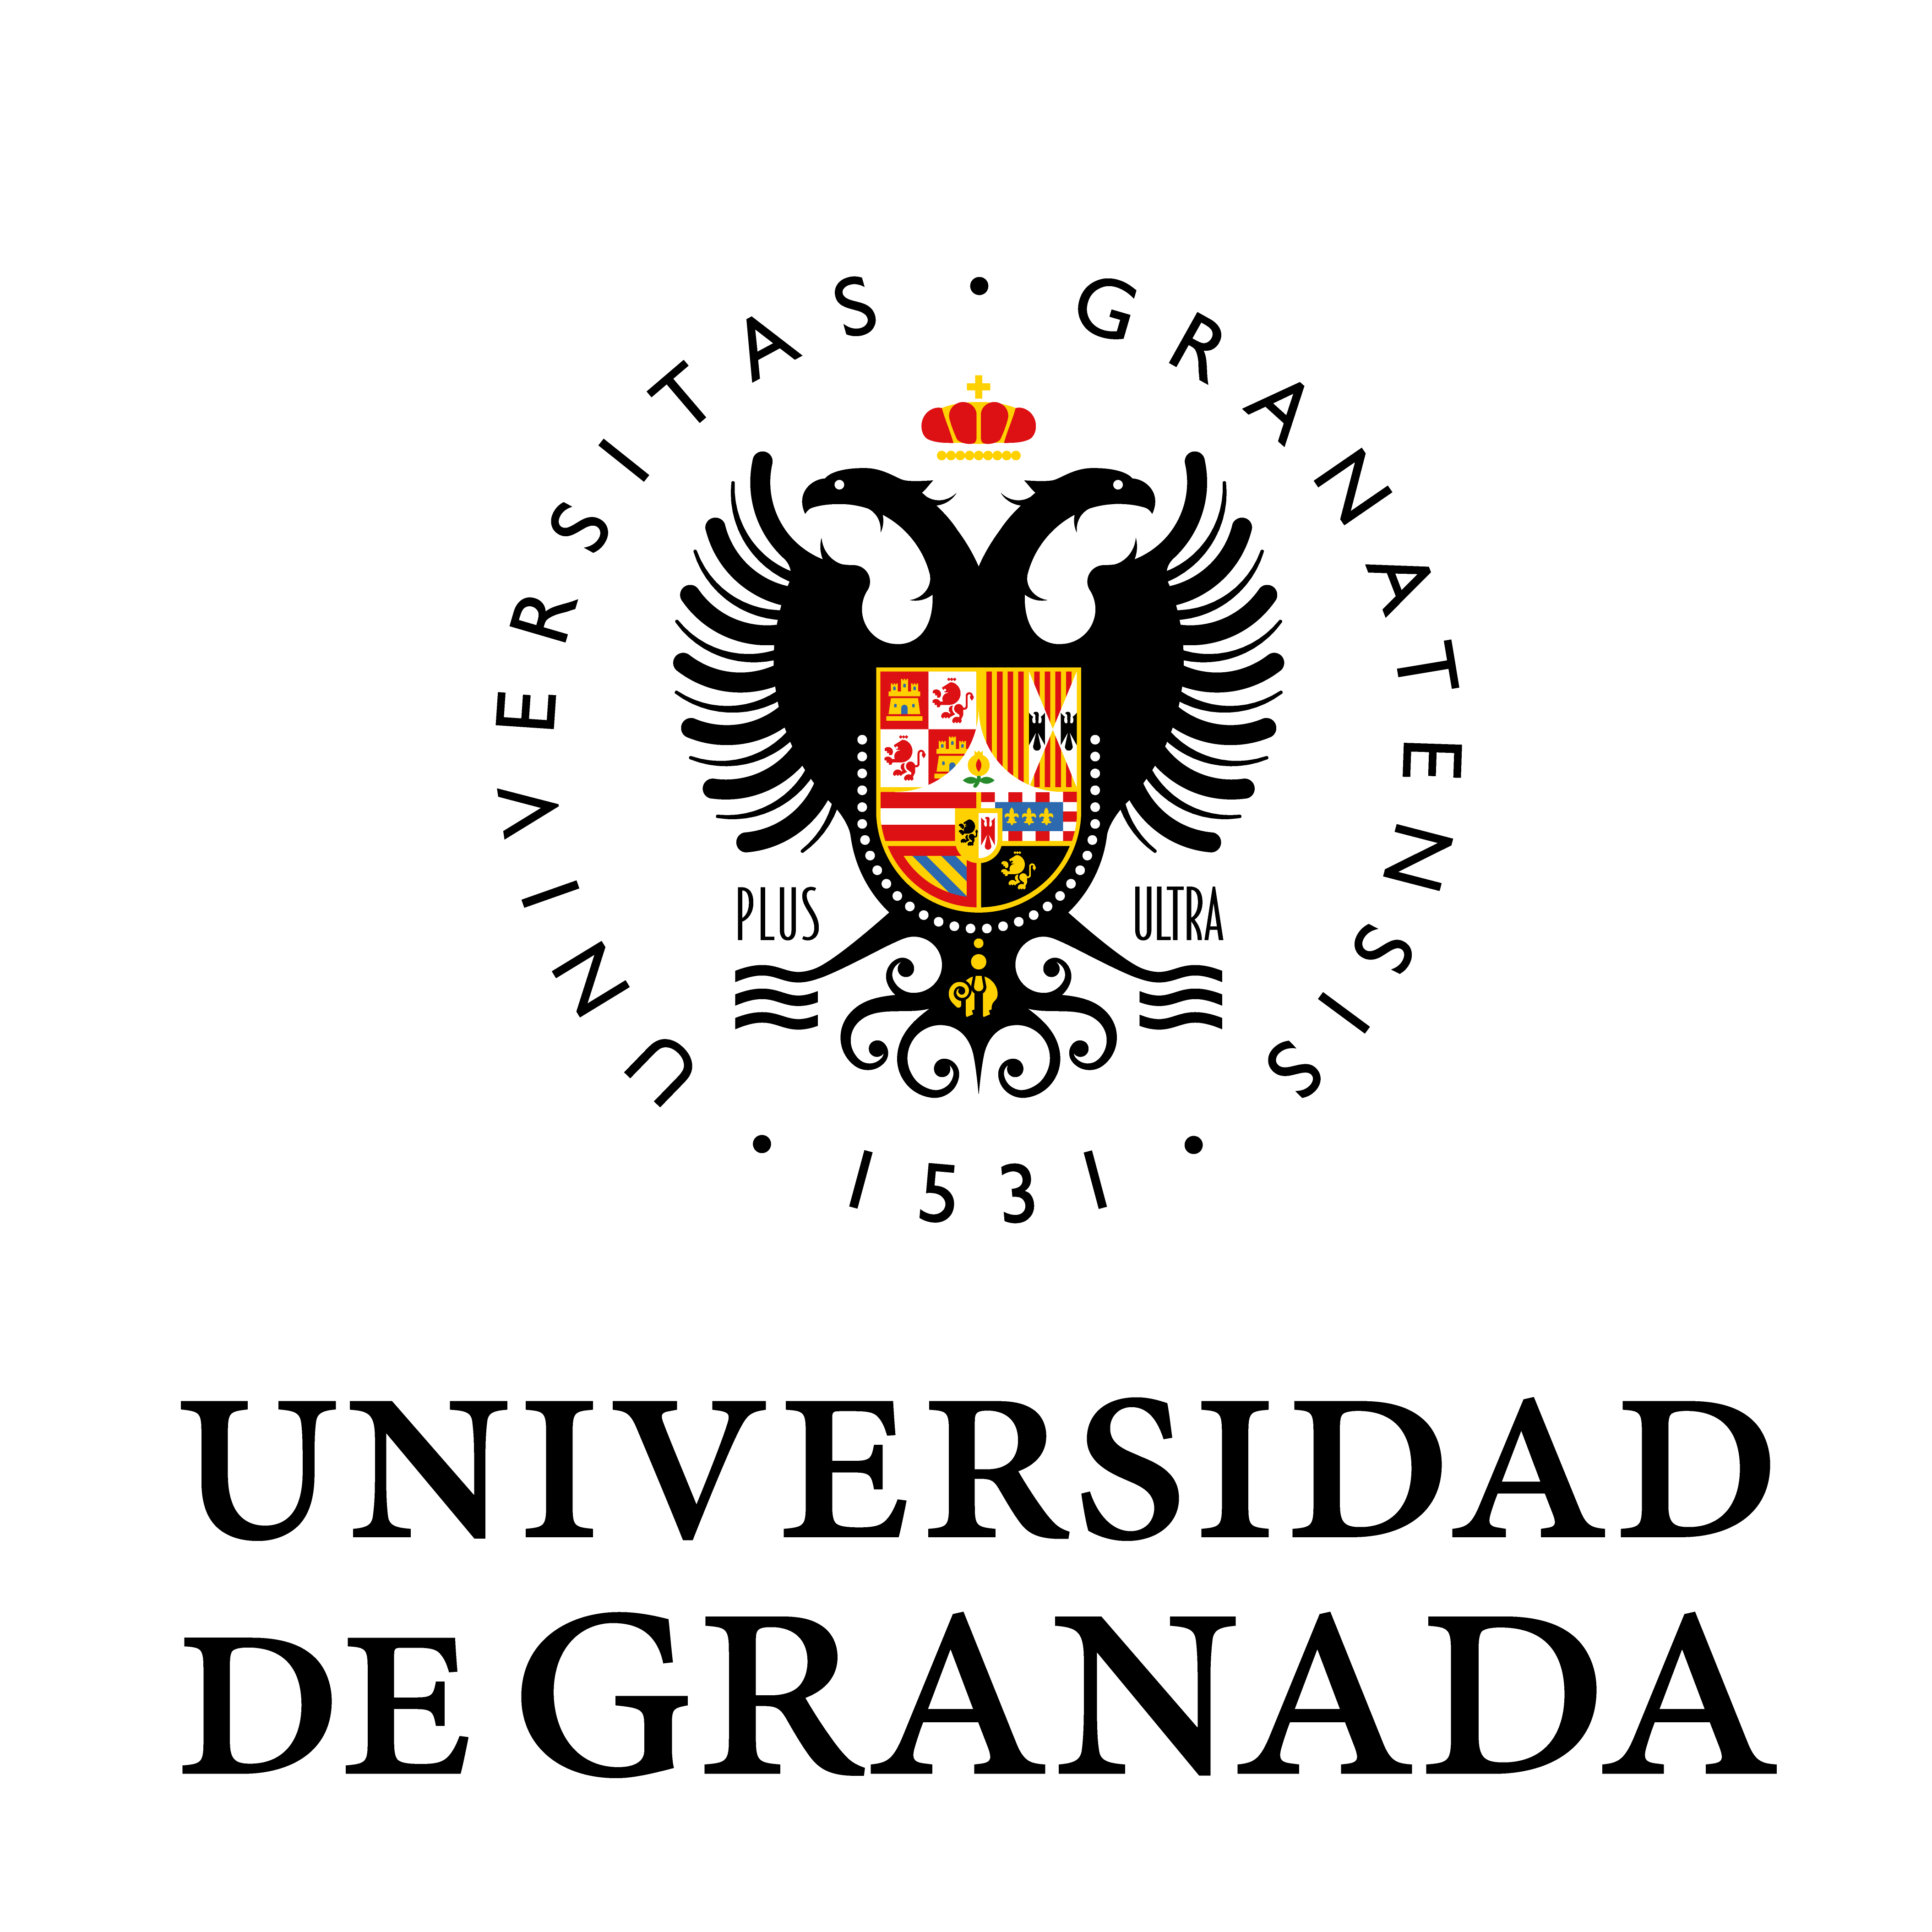
\includegraphics[scale=0.4]{img/logo_ugr.png}
\end{figure}

\begin{center}
  \Large TRABAJO FIN DE GRADO\\ 
  \large Doble grado en Ingeniería Informática y Matemáticas
  \vspace{0.7cm}

  \hrule
  \vspace{0.2cm}
  \textbf{\LARGE MW Store: facilitador genérico para proveedores de servicios con multi-inquilinato en una infraestructura Cloud}
  \vspace{0.2cm}
  \hrule
  \vspace{2cm}
  
  \textbf{Autor}

  Rubén Morales Pérez

  \vspace{2cm}
  \textbf{Director}

  Manuel Isidoro Capel Tuñón

  \textit{Departamento de Lenguajes y Sistemas Informáticos}
\end{center}

\newpage

\ 
\thispagestyle{empty}

Originality statement

\

Rubén Morales Pérez

\

I explicitly declare that the work presented as TFG,
corresponding to the academic year, is original, in the sense that no sources have been used for the preparation of the work without proper citation.

\

Granada September 3, 2022

\

Signed:


\newpage

Rubén Morales Pérez, student of the DGMII at the Universidad de Granada, with DNI 23308366M, I authorize the location of the following copy of my Master's Thesis % TODO?: Master or Dissertation?
in the library of the University so that it can be consulted by the persons who wish it.

\

Granada September 3, 2022

\

Signed:

\newpage


D. Manuel I. Capel (tutor), Profesor del Área de Lenguajes y Sistemas Informáticos del Departamento LSI de la Universidad de Granada.
Informa:

\

Que el presente trabajo, titulado "MW Store: facilitador genérico para proveedores de servicios con multi-inquilinato en una infraestructura
Cloud", ha sido realizado bajo su supervisión por Rubén Morales Pérez, y autorizo la defensa de dicho trabajo ante el tribunal que corresponda.
Y para que conste, expido y firmo el presente informe.

\

Granada September 3, 2022

\

Signed:

\newpage
\shipout\null % Empty page
\newpage

\textbf{MW Store: facilitador genérico para proveedores de servicios con multi-inquilinato en una infraestructura Cloud}

\

\textbf{Palabras clave}

\

Multi-tenencia, Concurrencia, Redes Petri Coloreadas, Modelos Matemáticos, Calidad de Servicio, Nube.

\

\textbf{Resumen}

\

La tendencia en informática hacia una externalización a la nube incentiva la adopción de ciertas prácticas en el desarrollo del software \cite{cloud-computing-state-of-the-art}.
La nube como concepto permite aumentar la seguridad informática gracias a la restricción de acciones y/o permisos a los que los usuarios tienen acceso.
La multi-tenencia reduce el coste del software compartiendo recursos como los servidores o las bases de datos entre los diferentes usuarios.
Hay varias propiedades deseables para garantizar buena calidad de servicio, como son la escalabilidad, elasticidad y tolerancia a fallos.
A la hora de gestionar la infraestructura para almacenar los datos hay varias consideraciones a tener en cuenta.
Los tenants pueden requerir configuración personalizada, scalabilidad de datos con réplicas y particiones, consistencia de datos, escalabilidad horizontal dinámica para responder ante aumentos de carga en el sistema.
Es necesario elegir entre la completa disponibilidad o consistencia de los datos.
Dependiendo de los requisitos funcionales del sistema las propiedades ACID y BASE influenciarán la elección de la base de datos adecuada.
La complejidad creciente del software requiere cierto esfuerzo para poder controlarla de forma efectiva.
Cualquier sistema reactivo (con o sin bases de datos) se puede modelar usando redes de Petri coloreadas (CPNs).
Este modelado matemático de los sistemas permite demostraciones formales de características deseables en aplicaciones del mundo real.
Ejemplos de dichas caracaterísticas son la disponibilidad de recursos, vivacidad y seguridad.
Las CPNs permiten entender las limitaciones de concurrencia de nuestros sistemas.
De esta forma se pueden diseñar sistemas capaces de resistir ingentes cantidades de peticiones por segundo. 
Este proyecto permite a las empresas crear una web con sus productos.
Los clientes de dichas empresas serán usuarios finales del sistema y podrán comprar los productos online en la página correspondiente de cada empresa.
MW-Store está modelado usando el software CPN Tools, un sistema gratuito disponible balo la licencia GNU General Public License (GPL) version 2.
CPN Tools ha ayudo a demostrar la correctitud del diseño de MW-Store verificando las propiedades deseables del sistema.
De esta forma, se han extraído conclusiones sobre la calidad de servicio del sistema implementado.


\newpage



\textbf{MW Store: generic handler for multi-tenant service providers in a cloud infrastructure}

\

\textbf{Keywords}

\

Multi-tenancy, Concurrency, Colored Petri Nets, Mathematical Modeling, Quality Of Service, Cloud.

\

\textbf{Abstract}

\

The trend toward outsourcing computing in the Cloud encourages the adoption of certain practices in software development.
The Cloud as a concept makes it possible to increase IT security by restricting the actions and/or permissions to which end users have access.
multi-tenancy reduces the cost of software by sharing resources such as servers or databases among different users.
There are relevant properties for adequate quality of service, like scalability, elasticity, and fault tolerance.
When it comes to data persistence, there are some trade-offs to consider.
Tenants might require custom extensibility, data scalability with replications and partitions, data consistency, and dynamic horizontal scalability to respond to increasing demands, which means transitorily changing the system’s load.
It is not possible to have both availability/latency and consistency in distributed data stores \cite{acid-base-database-transaction-processing}.
Depending on the functional requirements of a system, ACID or BASE properties will influence the initial decision of tenants' data store(s) implementation.
The increasing software complexity requires effort to manage it effectively.
Any reactive system (with or without a data store(s)) is modelable with Colored Petri Nets (CPNs).
This mathematical modeling of systems allows us to perform formal demonstrations of desirable features in real-world applications, e.g., resource availability, liveness and security.
CPNs allow us to understand the concurrency limitations of our systems.
In this way, systems can be designed to withstand huge amounts of requests per second.
The project allows companies to create a website with their products.
The customers of each tenant will be able to purchase those products online at the corresponding website.
MW-Store is modeled using the software provided by CPN Tools, a software under the GNU General Public License (GPL) version 2.
CPN Tools has assisted us in demonstrating the correctness of the MW-Store design by verifying the desirable properties and thus being able to draw conclusions about the quality of service of the implemented system.




\newpage
\shipout\null % Empty page
\newpage




\maketitle
\tableofcontents % Generando el indice
\setlength\parindent{0pt} % Quitamos la sangría


\newpage
\shipout\null % Empty page
\newpage

\section{Introduction}

Modern society's demands explain the tendency towards more complex and configurable software.
Configurability extends a system's functionality, including the possibility of simplifying the interfaces to handle just the specific requirements of each client.
Internet evolution as the standard communication network facilitates its adoption as an abstraction layer over the operating system.
Computation outsourcing to the Cloud has several advantages like increased security, no local installation, longer battery life, etc. \cite{humanes2016}.
The Cloud also creates a dependency on the Internet that might not be acceptable for all critical systems.
Virtualization is essential to offer web services on demand, improving resource efficiency and reducing overall business costs.

\

Cloud Computing and Software-as-a-Service (SaaS) influence is growing in enterprise software development.
SaaS is usually handled using multi-tenant paradigms. The formal definition of multi-tenancy (from \cite{defining-multi-tenancy}) is:

\

\definition{Multi-tenancy}{ ``property of a system where multiple customers, so-called tenants, transparently share the system’s resources, such as services, applications, databases, or hardware, with the aim of lowering costs, while still being able to exclusively configure the system to the needs of the tenant.'' \cite{defining-multi-tenancy}}

\

Each tenant handles its own customers' data.
In general, it is not possible to access data from other tenants' directly \cite{defining-multi-tenancy}.

\

Multi-tenancy helps to handle just one system to serve several clients at the same time \cite{shiller2011}.
% TODO: cite  (Shiller et al. 2011). 
This approach is also helpful in data layer access since it allows database management systems to handle several tenants with uneven requirements in just one place.
Sharing  data access layers helps to overall scalability.
The main drawback is that it makes tenants services dependent on the load of other tenants.
This dependency is handled with some scalability approaches.

\

Multi-tenancy still allows customization of the system behaviour to meet different customer requirements. Indeed, incremental software development approaches combined with tenant configuration allow custom interfaces for diverse clients. 
Even within the same field, some clients may need complex interfaces and requirements, while others may prefer simplicity.
From an economic point of view, this customization facilitates remarkably different bills adapted to the client's budget.
Multi-tenancy can be applied to several levels in a system’s architecture and there are different architectural approaches to define it.
It is possible to refer to multi-tenancy by using the whole picture of a system or by increasing the granularity to refer to the database level.
To properly use the term multi-tenancy, several core principles have to be covered: data isolation, scalability, concurrent data access, performance and security \cite{cloud-computing-state-of-the-art}.

\

\definition{NIST definition of Cloud Computing.}{ ``Cloud computing is a model for enabling convenient, on-demand network access to a shared pool of configurable computing resources (e.g., networks, servers, storage, applications, and services) that can be rapidly provisioned and released with minimal management effort or service provider interaction.'' \cite{cloud-computing-state-of-the-art}}

\

Infrastructure outsourcing provided by Cloud Computing tends to reduce risks like hardware failures, and becomes responsibility of  of the infrastructure providers \cite{cloud-computing-state-of-the-art}.
Virtualization allows Cloud Computing to pool computing resources and distribute them on demand to the applications.
Resources, like software, are now deployed off premise.
Dynamic resource provisioning can be either reactive, i.e. responsive to sudden demand variations; or proactive, allocating resources before they are needed by using demand forecast methods \cite{cloud-computing-state-of-the-art}.
Cloud Computing architecture (Figure \ref{fig:cloud-computing-architecture}) could be described in four layers \cite{cloud-computing-state-of-the-art}:

\begin{itemize}
    \item Hardware: handles the cloud physical resources \cite{cloud-computing-state-of-the-art}.
    \item Infrastructure/virtualization: pool of storage and computing resources, e.g. virtual machines \cite{cloud-computing-state-of-the-art}.
    \item Platform: operating systems and application frameworks \cite{cloud-computing-state-of-the-art}.
    It tries to reduce the effort to deploy applications.
    Platform as a Service (PaaS) provides these resources on demand.
    \item Application: the Cloud applications with Web interfaces \cite{cloud-computing-state-of-the-art}.
\end{itemize}

\begin{figure}[H]
  \centering
  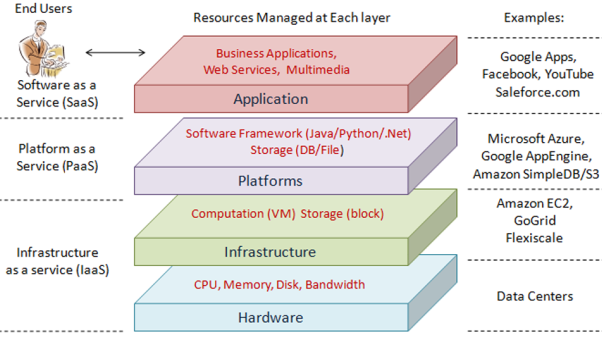
\includegraphics[scale=0.5]{img/cloud/cloud-computing-architecture.png}
  \caption{Cloud computing architecture \cite{cloud-computing-state-of-the-art}.}
  \label{fig:cloud-computing-architecture}
\end{figure}

From an economic perspective, economy-of-scale is easier to achieve by implementing Cloud-based solutions in huge data centers, which leads to better manageability \cite{cloud-computing-state-of-the-art}.
A disadvantage of this approach is the energy consumption and initial investments \cite{cloud-computing-state-of-the-art}, although the relative cost per server will hopefully be reduced or the necessary computing resources located in centers with lower electricity costs.
On the other hand, smaller data centers will not require that amount of power consumption and could be preferable in case of tight budget.
To prevent single points of failure and increase potential availability several smaller globally distributed data centers can be considered. 

% TODO
% Software as a Service (SaaS) as an outsourcing model: An economic analysis
% https://www.researchgate.net/publication/228447677_Software_as_a_Service_SaaS_as_an_outsourcing_model_An_economic_analysis

% Cloud Computing-Software as Service 
% https://www.researchgate.net/publication/274481004_Cloud_Computing-Software_as_Service

\subsection{Classification}
% TODO?:  SaaS Architecture Maturity Model


From the isolated approaches to more shared data \cite{multi-tenant-data-architecture}, multi-tenant data classification is a continuum:

\begin{itemize}
    \item Separate databases. Data isolation is easier to achieve using this approach. Generally, the application will execute the same code in the same server(s) for all the tenants, but this extra data security layer helps in data isolation. The main disadvantage is handling several connections to different databases, leading to higher maintainability costs. There is a limit on the number of databases that a single server can handle, a constraint that is not that important in other approaches.
    \item Shared Database, Separate Schemas.
    Database tables for each customer are grouped into a separated schema.
    This approach shifts security to the database permissions layer (like in the separate databases' scenario), and it is cheaper than separate databases \cite{cloud-computing-state-of-the-art}.
    It is the most used due to its trade-offs concerning resource usage, performance, and security.
    \item Shared Database, Shared Schema. Database tables store records from multiple tenants.
    A table column links each record with the appropriate tenant.
    This approach is the cheapest one, allowing the largest number of tenants per server.
    The higher number of rows per table is a limiting factor that could be reduced using indexes at database level.
    One disadvantage of this approach is that when customer requirements are very different, there is a performance overhead accessing the database.
    This overhead will be analyzed with the different extensibility patterns for multi-tenancy.
\end{itemize}

Some customers will have stronger data isolation requirements than others \cite{cloud-computing-state-of-the-art}.
Separate databases add an extra security layer due to more granularity in database access permissions.
Your business could take the decision based on expected requirements like the number of tenants, data per tenant, tailored tenant services, etc.
Separate databases or schemas would allow easier configurability per tenant, creating custom tables and columns as needed.
The business model is relevant here because more shared approaches would make \href{https://en.wikipedia.org/wiki/Feature_toggle}{feature toggle} straightforward, allowing turning on/off certain features on the fly.

\

On the other hand, just because a system is advertised as SaaS in the cloud does not mean it holds its benefits (savings, security, flexibility, disaster recovery, scalability, access to automatic updates, ...) \cite{saas-maturity-model}.
Microsoft describes an incremental SaaS maturity along three dimensions: configurability, multi-tenancy and scalability \cite{saas-maturity-model}. 
The axis of the maturity model combines the axis of the service component (core features to structure software) and the maturity levels (Figure \ref{fig:saas-maturity-model}) \cite{cloud-computing-state-of-the-art}:
\begin{itemize}
    \item Ad Hoc Level: dedicated database and schema. Each customer has access to a different application through Web interfaces. With respect to the Service-level agreement (SLA), it depends on separated contracts reflecting the requirements for each user.
    \item Standardization Level: attempts to provide shared service. It shares the database using dedicated schema with configurable single tenants, allowing users to build their service model.
    \item Integration Level: multi-tenant environment with shared database and schema. There is a predefined shared instance and configurable options for each tenant. The business layer focuses on measurable SLA adaptations.
    \item Virtualization Level: focus on scalability and availability with the possibility to include load-balancing.
    User requirements are handled in the business process (instead of code customization) and optimized SLA policies per customer.
\end{itemize} 

\begin{figure}[H]
  \centering
  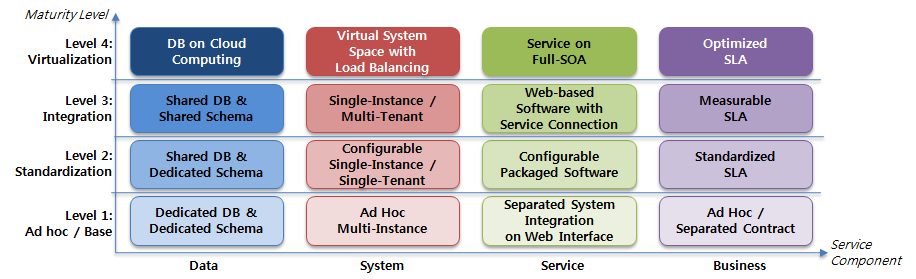
\includegraphics[scale=0.5]{img/cloud/saas-maturity-model.png}
  \caption{SaaS Maturity Model \cite{saas-maturity-model}.}
  \label{fig:saas-maturity-model}
\end{figure}

The different abstractions generated using these layers allows a PaaS provider to externalize the infrastructure to an IaaS provider and focus on their platform \cite{cloud-computing-state-of-the-art}.

\

Some service providers are focused on reducing overall costs, while others are more expensive but focused on higher reliability and security.
There clouds can be classified in several types \cite{cloud-computing-state-of-the-art}:
\begin{itemize}
    \item Public: offering resources to the public.
    \item Private (also called internal): exclusive for a given organization. They offer more control at a higher cost than the public ones.
    \item Hybrid: some Cloud components are public, and others are private. The separation must be designed in advance.
    \item Virtual private clouds (VPC): a virtualization layer over public clouds.
    It virtualizes servers, applications and the network.
\end{itemize}



\newpage



\section{Security}
SaaS models encourage businesses to shift their data management to another company.
Security must be considered to keep customer trust. 
As a rule of thumb, multiple defence levels against any potential threats increases security.

\

SaaS applications allows to shift security management to the back end.
This is a relevant change because one of the main security issues in computer sciences is end users.
Splitting the security by design in multiple servers prevent a single point of failure and makes it more difficult for users to grant too many permissions (CORS policy is important here).
Defence in the front end is still a nice to have, though.
In desktop applications the code could be potentially obtained by reverse-engineering and modified to meet certain goals. % Citation needed
Security in the front end is nice to have, but we must consider that any front end security can be bypassed.

\

Security must be considered by design, not to rely on security through obscurity.
There are several security patterns (agnostic to the database management system) available for each data isolation approach \cite{multi-tenant-data-architecture}.
In the scenario of multi-tenancy, these security approaches should be taken into account to provide security at different levels:
\begin{itemize}
    \item Filtering: the communication between each tenant and the data source is restricted to an intermediary layer, allowing access only to their tenant data by design.
    It is possible to implement this by design in the code, using database access objects with automatic tenant identifiers filtering.
    Filtering should not depend on the ability of the programmer.
    The tenant id could be required for each request to the back end.
    For additional security, this tenant id can be stored in a temporal token previously generated and encrypted in the back end.
    \item Permissions: use access control lists (ACLs) to determine access data.
    Another desirable layer of security are Virtual Private Networks with Two-Factor Authentication.
    \item Encryption: cipher critical data in the database will prevent unauthorized individuals to extract information about the tenants even in case of data leaks.
\end{itemize}

Some security patterns are applicable in all the scenarios (Separate Databases, Shared Database with Separate Schemas and Shared Database with Shared Schema) \cite{multi-tenant-data-architecture}:
\begin{itemize}
    \item Trusted Database Connections
    \item Secure Database Tables
    \item Tenant Data Encryption
\end{itemize}

Each scenario will be described below.

\subsection{Trusted Database Connections}
Impersonation is one method to improve security accessing databases information (Figure \ref{fig:impersonation-database-access}).
In this approach, individual database users are granted with granular permissions at different levels: procedures, queries, views and tables.
Any call to the database use the user's security context.
It is possible to create a database user for each tenant, restrict its access only to strictly required stuff and modify the data layer of the code to use different database tenant accounts when pooling connections to the database.

\

Another approach is the trusted subsystem access method (Figure \ref{fig:trusted-subsystem-database-access}).
In this scenario, database connections always use the application identity, without extra distinction for different tenants.
It is still possible to increase security at code level using an extra permission layer (i.e. encrypted tokens generated in the back end), though.
It is easier to handle but it would not allow deeper permission granularity at the database level, though.

\begin{figure}[h]
    \centering
    \begin{minipage}[t]{.5\textwidth}
      \centering
      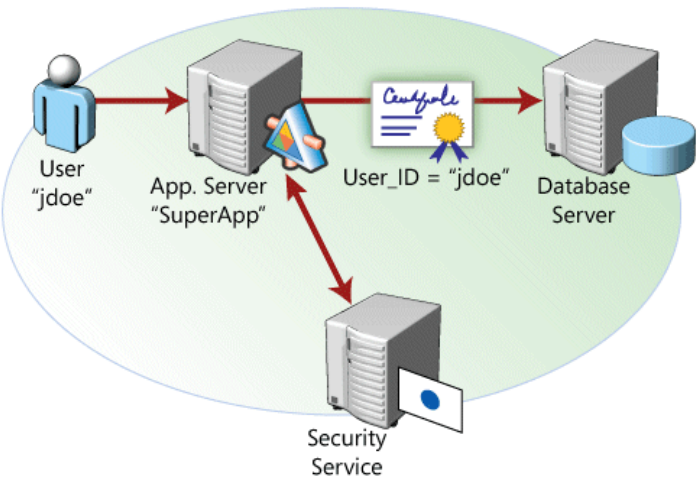
\includegraphics[width=0.75\linewidth]{img/db/impersonation-database-access.png}
      \caption{Impersonation database access \cite{multi-tenant-data-architecture}.
      \label{fig:impersonation-database-access}}
    \end{minipage}%
    \begin{minipage}[t]{.5\textwidth}
      \centering
      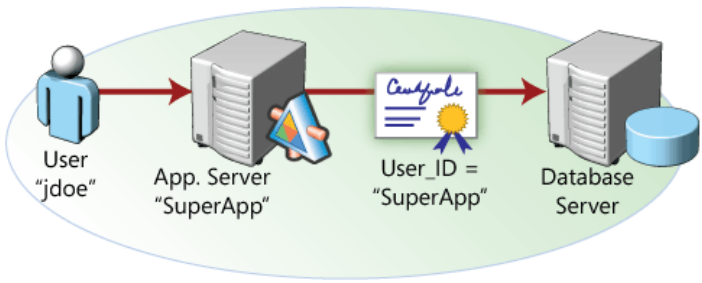
\includegraphics[width=1\linewidth]{img/db/trusted-subsystem-database-access.png}
      \caption{Trusted subsystem database access \cite{multi-tenant-data-architecture}. \label{fig:trusted-subsystem-database-access}}
    \end{minipage}
\end{figure}


\subsection{Secure Database Tables}
It is possible to secure a database with table granularity using the SQL GRANT command.
The following command will add access to a database user using the access control list for a given table.
It grants restricted access only to a specific tenant user account:
\begin{lstlisting}[language=sql,numbers=none]
GRANT SELECT, UPDATE, INSERT, DELETE ON [Table] FOR [User]
\end{lstlisting}

It is possible to restrict tenant access using database views.
A view is a virtual table showing the results of a query \cite{views-in-sql}, selecting rows from one or more tables. These views are not stored physically in the database.
If there is a table called \textit{Table} and several tenants \{Tenant1, ..., TenantN\} it is possible to prevent direct read access to \textit{Table} and create several views 
$$\{Tenant1TableView,\ ... \ ,\ TenantNTableView\}.$$
Each TenantXTableView will be the result of a SELECT query filtering with the tenant id column.

\

\begin{lstlisting}[language=sql,numbers=none]
CREATE VIEW Tenant1TableView AS
    SELECT * FROM Table WHERE tenant_id = get_current_tenant_id()
\end{lstlisting}

\

where \textit{get\_current\_tenant\_id()} is a procedure returning the current tenant identifier.
A possible approach to define that procedure would be to create an intermediate table linking tenant ids with database users (using the security identifier SID of the database connection).
It is possible to avoid the extra table directly hard coding the tenant id in the filter, but it would be less secure.
It is relevant to highlight that only read access could be restricted using this approach because the tenants still need to insert and update rows in the original table.

\ 

Malicious/mistaken UPDATE, INSERT, DELETE statements could be prevented using a similar methodology with triggers (shown in Figure \ref{fig:tenant-triggers-data-isolation})

\begin{figure}[h]
\centering
\begin{minipage}[t]{.31\textwidth}
\centering
\begin{lstlisting}[language=sql,numbers=none]
DELIMITER $$

CREATE TRIGGER TENANT_PREVENT_INSERT
    BEFORE INSERT
    ON Table FOR EACH ROW
BEGIN
  IF NEW.TenantID != SUSER_SID() THEN  
    -- Throw error
  END IF;
END$$    

DELIMITER ;
\end{lstlisting}
\end{minipage}%
\hspace{0.3cm}
\begin{minipage}[t]{.31\textwidth}
\centering
\begin{lstlisting}[language=sql,numbers=none]
DELIMITER $$

CREATE TRIGGER TENANT_PREVENT_UPDATE
    BEFORE UPDATE
    ON Table FOR EACH ROW
BEGIN
  IF OLD.TenantID != SUSER_SID() THEN  
    -- Throw error
  END IF;
END$$    

DELIMITER ;
\end{lstlisting}
\end{minipage}
\hspace{0.3cm}
\begin{minipage}[t]{.31\textwidth}
\centering
\begin{lstlisting}[language=sql,numbers=none]
DELIMITER $$

CREATE TRIGGER TENANT_PREVENT_DELETE
    BEFORE DELETE
    ON Table FOR EACH ROW
BEGIN
  IF OLD.TenantID != SUSER_SID() THEN  
    -- Throw error
  END IF;
END$$    

DELIMITER ;
\end{lstlisting}
\end{minipage}
\caption{MySQL base trigger examples to prevent insert/update/delete different tenant data.}
\label{fig:tenant-triggers-data-isolation}
\end{figure}


\subsection{Tenant Data Encryption}
Cryptography can be used as a security layer and there are two main approaches:
\begin{itemize}
    \item Symmetric: only one key is created, using it for encryption and decryption of data \cite{multi-tenant-data-architecture}.
    \item Asymmetric (public‐key cryptography): Two linked keys are generated, the public key will encrypt, and the private key will decrypt the data.
    Both keys are interchangeable.
    It is theoretically possible to encrypt with the private key and decrypt with the public one. The term "private" is just a reference to differentiate both keys.
\end{itemize}

Asymmetric cryptography is slower than symmetric cryptography and could not fit in applications where performance is considered.
In multi-tenancy is possible to add extra encryption security by creating different keys, one per tenant.
It is more difficult to manage, though.


\newpage
\section{Extensibility}
Extensibility measures effort required to extend a system's behaviour.
Extensions of system's functionality increase the complexity and could make software maintainability harder.
It is desirable to use one of the SOLID principles: Open-closed.
Open-closed principle states that a system should be open for extension but closed for modification, preventing possible regressions in legacy code.
An extensible design provides a framework to allow changes \cite{philosophy-extensible-software}, small increments will improve software reusability.

\

Traditional software development requirements will be needed for appropriate extensibility \cite{philosophy-extensible-software}:
\begin{itemize}
    \item High cohesion: degree to which part of the code forms a logically single and atomic unit.
    Example: classes that contain strongly related functionalities help to keep related parts of a code base in a single place. % https://www.educative.io/edpresso/definition-high-cohesion
    % TODO?: describe types of cohesion
    \item Low coupling: degree of interdependence between software modules. % https://en.wikipedia.org/wiki/Coupling_(computer_programming)
    Changes in more independent modules will not heavily impact other modules. % https://medium.com/clarityhub/low-coupling-high-cohesion-3610e35ac4a6
    \item Interface-implementation separation allows you to change the implementation independently of the interface. 
    Polymorphism allows several implementations of the same interface to do similar things in different ways. % https://softwareengineering.stackexchange.com/questions/142192/why-would-a-programmer-want-to-separate-implementation-from-interface
    \item Dependencies: external dependencies are often needed to perform specific tasks.
    When a system grows is usually divided into several components, there will be internal inter-dependencies.
    It is possible to automatically generate the dependency graph in order to inspect coupling or dangling dependencies. External dependencies tracking allows for the recognition of possible migrations to avoid non-maintained or vulnerable dependencies.
    Extensibility would lead to fewer and cleaner dependencies and well-defined interfaces \cite{philosophy-extensible-software}.
    \item Procedures to perform continuous integration: increase the pace and safety of code integration from several contributors in a system.
    Usage of automated tools for build, test and code analysis will allow faster feedback on new code’s correctness \cite{what-is-continuous-integration}.
    Continuous Integration (CI) helps to achieve agile approaches for software development processes.
    The next step is Continuous Delivery, ensuring that software is always ready to be delivered.
    Continuous deployment will be the last step of this pipeline.
    In this phase, the software artifact(s) will be automatically launched and distributed to end-users when tests pass \cite{what-is-continuous-integration}.
\end{itemize}

% TODO?: maximizing extensibility by means of design principles
% https://gupea.ub.gu.se/bitstream/handle/2077/20561/gupea_2077_20561_1.pdf;jsessionid=B2EA963686F0191DEED06BD96E805F6F?sequence=1

\

The extensible design fits well with Agile methodologies and iterative development, allowing dynamic prioritization \cite{philosophy-extensible-software} by looking at software as a growing entity.


\subsection{Multi-tenancy customization}
It is possible to conditionally extend the functionality of a tenant by adding new features or modifying existing ones.
There will be a set of tables/columns at the core of the application, but customized customer cannot always be addressed with a rigid data model.

\

There are several ways to extend the data model to handle custom functionality \cite{multi-tenant-data-architecture}:
\begin{itemize}
    \item Preallocated Fields
    \item Name‐Value Pairs
    \item Custom columns
    \item Columns with JSON type
    \item NoSQL databases
\end{itemize}

\

The data model can be customized creating personalized columns in certain table(s) to grant tenants extended functionality \cite{multi-tenant-data-architecture} (Figure \ref{fig:preallocated-database-fields}).
This black box approach allows determining how to use these fields depending on each customer, hiding actual data model complexity.
Nullable strings could be used as a flexible data type for the custom fields, avoiding unnecessarily data type restrictions (castings can be done in the code).

\begin{figure}[H]
    \centering
    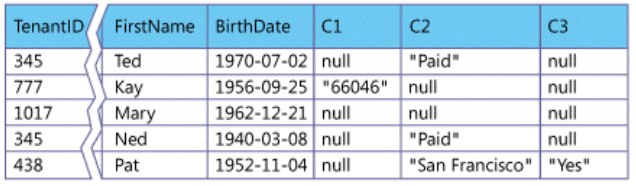
\includegraphics[scale=0.5]{img/db/extensibility/preallocated-fields.png}
    \caption{Database table with preallocated fields C1, C2 and C3 \cite{multi-tenant-data-architecture}}
    \label{fig:preallocated-database-fields}
    % TODO? generate figure with https://dbdiagram.io/d for uniform style
\end{figure}

\

Too few custom fields restrict tenants' customizability.
Too many custom fields will lead to a sparse database with many unused fields.
Name‐Value pairs allow creating the desired customizable fields for each tenant \cite{multi-tenant-data-architecture} using one to many relationships with an external table (Figure \ref{fig:name-value-pairs-database}).
The number of pairs is limited by the maximum length allowed in the database for the name column. Actually this is not a relevant restriction because a tenant will not have millions of custom fields.
When a record from \textit{original\_table} is fetched, a lookup in the table \textit{name\_value\_table} will select all name-value pairs corresponding to the id of the external reference (lazy or eager loading can be used, depending on the specific use case).
It is a good approach when specific customers require considerable flexibility, and the shared database approach is used. 
The disadvantages of name-value approach are:
\begin{itemize}
    \item Black box approach with hidden types and possible database relationships
    \item Possible anti-pattern in the code:
\begin{lstlisting}[language=python,numbers=none]
if isTenant1():
    ...
elif isTenant2():
    ...
\end{lstlisting}
\end{itemize}

\begin{figure}[H]
    \centering
    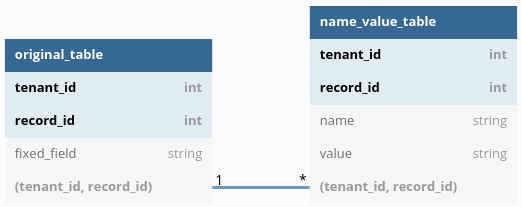
\includegraphics[scale=0.5]{img/db/extensibility/name-value-pairs.png}
    \caption{Tenants custom fields using name-value pairs \cite{multi-tenant-data-architecture}}
    \label{fig:name-value-pairs-database}
\end{figure}

\begin{comment}
% Source code to generate schema in https://dbdiagram.io/d
Table original_table {
  tenant_id int [pk]
  record_id int [pk]
  fixed_field string
}

Table name_value_table {
  tenant_id int [pk]
  record_id int [pk]
  name string
  value string
}

Ref: name_value_table.(tenant_id, record_id) > original_table.(tenant_id, record_id)
\end{comment}

\

Another extensible data model pattern is adding tailored columns to tenants' tables (Figure \ref{fig:custom-database-columns}).
The tailored database columns approach can be considered more appropriate in separate database/schema scenarios.
There would be extra unneeded fields for several customers in a shared database environment when different tenants have radically different requirements.
With a shared database, the database complexity would be the sum of all the tenants' complexities because it would include all the tailored columns.
It should be possible to add these features dynamically to the clients, and the code must work regardless of the combination of the features (if there are no incompatibilities).
Therefore the inner code complexity is similar with all the strategies used to separate tenants' data.

\begin{figure}[H]
    \centering
    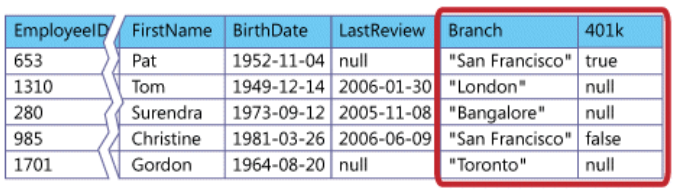
\includegraphics[scale=0.5]{img/db/extensibility/custom-database-columns.png}
    \caption{Custom database columns extensibility approach \cite{multi-tenant-data-architecture}}
    \label{fig:custom-database-columns}
\end{figure}

From a performance point of view, a customer with simple requirements might not need the database overhead of extra database columns. 
With entire custom database tables, the possible overhead can be reduced at the code level using lazy loading and preventing N+1 issues (unnecessary database calls while iterating over a collection of entities, fetching external reference entities in a loop instead of a single fetch).
The overhead is not a big deal in practice.

\

Databases can store JSON values using either strings (needs to be manually deserialized after fetch) or with native JSON types for database column definition.
The JSON format allows storing dynamic fields using a tree structure.
Some databases, like PostgreSQL, allow storing JSON in a native format, offering custom queries to filter data using the key/values of the JSON cells.
That native approach is better than directly storing the JSON as a string.
It also provides flexibility inside data structured in tables.

\

Another possibility to customize client requirements is to use NoSQL databases.
The relational model in SQL databases allows for more structured data since the database contains foreign keys \cite{comparison-query-performance-relational-and-non-relational-databases}.
On the other hand, NoSQL databases do not have these foreign keys, allowing more flexibility while storing data \cite{comparison-query-performance-relational-and-non-relational-databases}.
This flexibility relegates the responsibility of checking the possible relationships between the data manually in the code, but it is a good fit for non-structured data.
In other section, the performance differences of SQL versus NoSQL databases will be covered.

\   

Any custom field will lead to changes in the business logic, the presentation logic, or both, regardless of the extensibility pattern(s) used.
Any change to the business logic increases the entropy of the system and increases the risks of including software regressions.

% TODO?: Configurability in SaaS (Software as a Service) Applications
% https://sci-hub.hkvisa.net/10.1145/1506216.1506221


\subsection{Software regressions}
A software regression is a special type of bug where a certain feature was working before and stops working.
Regressions can be produced due to changes in the code or the environment (i.e. system upgrades, environment variables, ...).
Regressions can be classified in:
\begin{itemize}
    \item Functional: a feature that is no longer working.
    \item Performance: a feature is still working but more slowly or uses more resources (i.e. memory) than before.
\end{itemize}

Testing can reduce regressions likelihood, and tests are either manual (sometimes involving Quality Assurance positions) or automatic.

\subsubsection{Automatic testing}
Automatic tests will catch bugs before production release.
Several strategies that can be used:
\begin{itemize}
	\item End to end tests (E2E): involves entire workflows, typically front end, back end and database(s).
	\item Integration tests: specific use cases involving several system components.
	\item Unit tests: test cases involving only one component, mocking other components.
	For example: in the back end, the database calls are fake (just mocked), making the tests much faster.
\end{itemize}

A convenient relationship between the number of tests for each strategy is shown in the test pyramid:
\begin{figure}[H]
  \centering
  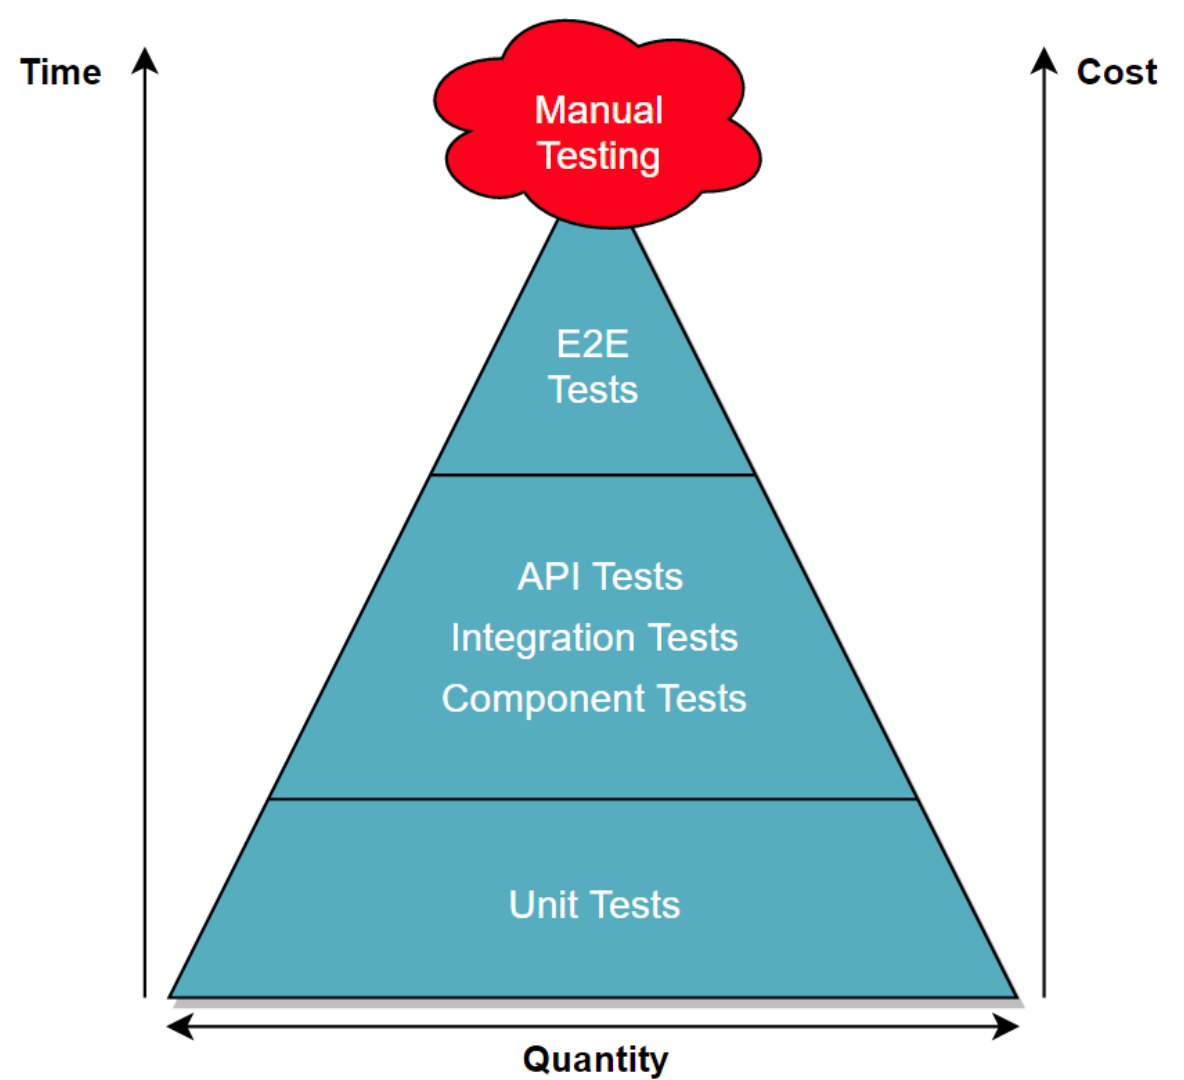
\includegraphics[scale=0.2]{img/test-pyramid.png}
  \caption{Test pyramid \cite{test-pyramid}.}
\end{figure}

The inverted testing pyramid (fewer unit and integration tests, with an emphasis on automated and manual functional testing) is considered an anti-pattern, reducing the responsiveness, maintainability, and reliability of the test setup \cite{test-pyramid}. 
Unit tests help identify faults in earlier phases \cite{test-pyramid} and must be the backbone of any software product.

\

Regression testing validates that new changes applied to a program do not break existing logic \cite{an-overview-of-regression-testing}.
Unit tests can be introduced in the continuous integration loop because their feedback is almost instantly.
End to end and integration tests do not scale well.
so it is not always possible to include all of them in the continuous integration loop.
Regression test selection techniques reduce the cost in time by selecting only the tests related to a modified program (i.e. two consecutive commits in a version control system) \cite{regression-test-selection}.

\

Other types of tests should also be considered \cite{types-of-software-testing}:
\begin{itemize}
	\item Performance tests: check the system when it is under significant load, they are quite costly to implement and run. % https://www.atlassian.com/continuous-delivery/software-testing/types-of-software-testing
	\item Smoke tests: check basic functionality of the application. % https://www.atlassian.com/continuous-delivery/software-testing/types-of-software-testing
	\item Security Testing: check how the system reacts to internal and/or external threats (i.e. penetration testing). % https://www.softwaretestinghelp.com/types-of-software-testing/#1_Security_Testing
	\item Mutation tests: it is a formal way to measure the quality of existing tests, weak tests can produce a false sense of safety.
	The code of a program is slightly modified, which is called a mutant, and then the tests are run.
	If the tests are robust enough, at least one should fail and the program modification is called a killed mutant.
	It is measured as
	$$Mutation\ score := \frac{Killed\ mutants}{Total\ number\ of\ mutants} \cdot 100.$$
	This approach inherits the scalability of the tests, and it is more suitable to verify unit tests.
% https://www.softwaretestinghelp.com/types-of-software-testing/#1_Security_Testing
\end{itemize}

The code of a program can be described as a graph \cite{regression-test-selection}.
Two different commits using a version control system are two different programs, i.e. they are represented as two graphs.
A rest API call (or any user action that only requires code execution in the front end) towards this program can be represented as a path inside this graph.
An integration test or end-to-end test can be represented as an ordered set of paths within one graph.
A pull request (updated with respect to the pull request destination branch) represent a different program. Therefore it is possible to extract a subset of the integration/end-to-end tests in order to detect regressions earlier and with lower costs.
This approach is more clever than traditional ones to handle slow tests, like smoke tests (although they are compatible approaches), because it is possible to run only the tests whose behaviour will change after merging.

\

Software programs tend to be more complex over time.
The number of tests won't (or should not) be reduced, but systematic approaches to handle this complexity are definitely nice to have.
Sometimes it will still be infeasible to run all the tests (ex. changes in one core part of the program) before merge a pull request.
In those scenarios it is possible to select a subset of tests maximizing the edges of the graph covered.
At a certain level of development the execution time of slow tests will force teams to schedule its execution daily, weekly, etc.
This approach allows to statically analyze the possible root cause(s) when tests fail, searching the commits that modified the parts of the graph involved in these tests.

% TODO?: talk about extensibility granularities
% TODO?: talk about feature flags


\newpage

\section{Concurrent systems modeling with Petri Nets}
In pure functional programming paradigms, a program is a composition of pure functions.
A pure function verifies two properties:
\begin{itemize}
    \item For the same input value(s), the output is always the same.
    \item There are no side effects, no variable/state outside of the scope of the function mutated after the function application.
\end{itemize}

A pure function can be considered equivalent to a mathematical function.
This approach allows certain optimizations like lazy evaluation or memoization.
On the other hand, functional programming cannot fully use pseudo-random numbers (since they usually use the execution time as a seed for randomization) or program state.
Program state is a source of potential failures and should be avoided when possible, but most the programs depend on databases continuously changing their state.

\ 

Most of the content of this section is inspired in the lecture notes of the subject 'Concurrent programming' provided by Manuel Isidoro Capel Tuñón in \cite{lecture-notes-concurrent-systems-validation}.
A reactive system interact with the environment, it cannot be represented as a composition of pure functions.
Concurrent systems are a subset of reactive systems, there are sequential reactive systems that are not concurrent.

\

\definition{Fair Transition System (FTS).}{ It is a quadruple $(\Sigma,\ T,\ \Sigma_0,\ R)$ where
\begin{itemize}
    \item $\Sigma$ is a set of states. 
    The state represents the value of the system variables at a precise moment.
    \item $T$ are the transitions of the system. A transition, $t\in T$, is a function
    $$t:\Sigma\rightarrow 2^{\Sigma} \hspace{1cm} (2^{\Sigma} \text{ represents all the possible subsets of } \Sigma),$$
    from a state $s\in\Sigma$ to a subset of $\Sigma$, $t(s)$.
    The subset $t(s)$ is called the successors of $s$.
    \item $\Sigma_0$ are the possible initial states of the system, $\Sigma_0 \subseteq \Sigma$.
    \item $R$ are the correctness requirements of the system. They limit the frequency of transitions.
\end{itemize}}

\

A Fair Transition System can represent any king of concurrent system, based on shared memory or message passing \cite{lecture-notes-concurrent-systems-validation}.
In FTSs is possible to define an execution:

\

\definition{FTS execution.}{ A sequence of states connected by transitions:
$$\sigma:s_0
\ \overset{t_0}{\longrightarrow} s_1
\ \overset{t_1}{\longrightarrow} s_2
\ \overset{t_2}{\longrightarrow} \  \dots \hspace{1cm} s_i\in\Sigma, t_i\in T.$$}

\

An execution represents the evolution of the global state of a system after several transitions.

\subsection{Petri Nets}
Studying the structure of Fair Transition Systems and its possible executions will provide relevant properties about the system's correctness.
The first approach to study these systems are Petri Nets.
% TODO: verify, this sentence is not true: A special kind of Fair Transition Systems is Petri Nets.

\

\definition{Petri Net}{ is a directed multigraph (a graph with two kinds of nodes) with annotations \cite{lecture-notes-concurrent-systems-validation}. It is defined as a 4-tuple $(P,\ T,\ I,\ O)$ where 
\begin{itemize}
    \item $P := \{p_1,\ ... \ ,\ p_n\}$ are the places (first kind of node), they represent the state variables of a discrete event system.
    \item $T := \{t_1,\ ...\ ,\ t_m\}$ are the transitions (second kind of node) transforming the values of the places.
    \newline
    \newline
    The arcs of the Petri Net are defined in the set $A$,
    $$A \subseteq \{T\times P\} \cup \{P\times T\}.$$
    As a consequence, the arcs only connect places with transitions (and vice versa).
    Arcs between two places or two transitions are not allowed.
    \item $I(t_j) := \{p : (p, t_j) \in A\}$ input function (or preset), it is the set of input places for a transition.
    \item $O(t_j) := \{p : (t_j,p) \in A\}$ output function (or post-set), it is the set of output places for a transition.
    \newline
    \newline
    A transition $t\in T$ is considered a fork when $|O(t)| > 1$, when $|I(t)| > 1$ it is considered a join.
    Respectively, for places, a place $p\in P$ is considered a collector when $|I(p)| > 1$, when $|O(p)| > 1$ it is considered a distributor.
\end{itemize}}

\begin{figure}[H]
    \centering
    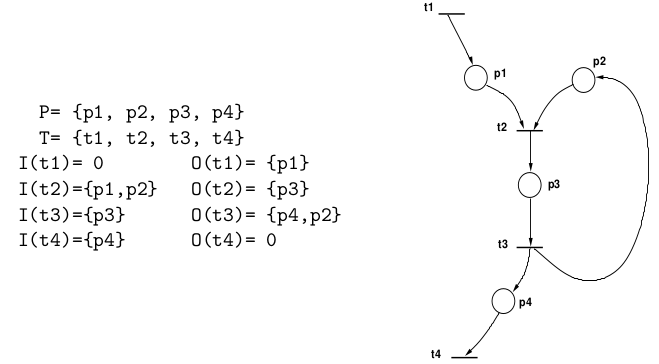
\includegraphics[scale=0.525]{img/petri-net/petri-net-example.png}
    \caption{Graphic representation of a Petri Net.}
    \label{fig:petri-net-example}
    % TODO?: Choose a simpler net, define the places, transitions of methods in latex (not image).
\end{figure}

Petri Nets can describe dynamic systems using discrete events.
It is possible to add concurrency restrictions in the interactions between these asynchronous events.
The mathematical nature of Petri Nets allows us to analyze the systems using different king of Petri Nets: P/T, High-Level PN, Colored Petri Nets, Timed Petri Nets, etc.

\

\definition{Pure Petri Net}{, it is a Petri Net where there is no place simultaneously being the input and the output of a transition.}

\

\definition{Regular Petri Net}{, it is a Petri Nets with a maximum of one arc per direction between a place and a transition.}

\

One arc starting at place $p_i$ to transition $t_j$ and other arc from $t_j$ to $p_j$ is a valid combination in regular Petri Nets.
The Figure \ref{fig:petri-net-example} represents a pure regular Petri Net.

\subsection{Marked Petri Nets}
To study the executions in Petri Nets, we need to define the marks stored in their places.
Intuitively, these marks will describe the state of the net at a given time.
The mark distribution represents the number of marks for each place of the Petri Net at a given moment.
A marking $M$ is represented as a vector, $M = (M_1, ..., M_{|P|})$, where each element $M_i\in\mathbb{N}_0^+$ represents the number of marks at place $p_i$.
Formally, the marking function is
$$M: P \rightarrow \{0,\ 1,\ ...\ ,\ |P|\}$$
$$M(p_i) := M_i,$$

and it represents the current global state of a system.
This definition allows us to define Marked Petri Nets as follows:

\

\definition{Marked Petri Net}{ is a special kind of Petri Net with an initial marking.
It is formally described as a 5-tuple $R := (P,\ T,\ I,\ O,\ M_0)$ where $M_0$ is the initial marking.}

\

In some specific nets, a place has its marking dependent on the marking of other places.
They are called implicit places and, under
certain circumstances, can be removed from the net without changing its behaviour \cite{lecture-notes-concurrent-systems-validation}.

\

An example of a graphical representation of a Marked Petri Net is shown in Figure \ref{fig:marked-petri-net-example}.

\

\begin{figure}[H]
    \centering
    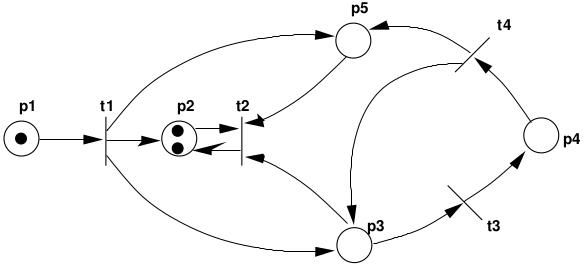
\includegraphics[scale=0.5]{img/petri-net/mpn/marked-petri-net-example.png}
    \caption{Marked Petri Net with one mark at place $p_1$ and two marks at place $p_2$ \cite{lecture-notes-concurrent-systems-validation}.}
    \label{fig:marked-petri-net-example}
\end{figure}

\

Now, some definitions are required to describe the executions in Marked Petri Nets.
The multiplicity, 
$$n: P\times T \rightarrow \mathbb{N}_0^+$$
$$n(p, t) := | [ x : x\in O(p) \ \wedge \ x=t ] |$$
is the number of arcs from one place to a transition.
There is an essential property of transitions related to multiplicity:
$$t\in T \text{ is enabled } \hspace{1cm} \Longleftrightarrow \hspace{1cm} \forall p\in I(t)\hspace{0.5cm} M(p) \geq n(p, t).$$

\

\definition{Reachability set of a Marked Petri Net.}{ Given a Marked Petri Net $R=(P,\ T,\ I,\ O,\ M_0)$, the reachability set $\mathcal{M}(R, M_0)$ is the set of all the reachable markings starting from $M_0$.}

\

A transition can be fired if and only if it is enabled.
The marking $M$ of the net will change following this function:
$$
\delta (M,t) : \mathcal{M} (R,\ M_0) \times T\ \rightarrow\ \mathcal{M} (R,\ M_0)
$$
$$
\delta (M,t) := 
     \begin{cases}
       M(p) + n(p,t) &\quad\text{ if } p\in O(t) \wedge p\not\in I(t)\\
       M(p) - n(p,t) &\quad\text{ if } p\not\in O(t) \wedge p\in I(t)\\
     \end{cases}.
$$

\

Intuitively, we can think of transition firing as a way to get one mark from each input place and transform them to one mark for each output place.
Clearly, the total number of marks in the net changes when a transition $t$ is fired and verifies $|I(t)| \not= |O(t)|$.
We can use Figure \ref{fig:marked-petri-net-transition-firing-example} to see an example of a transition firing.
The transition $t_1$ is enabled because all its input places ($\{p_1\}$) have a number of marks (one) greater or equal than the number of arcs from $p_1$ to $t_1$ (one).
After the firing, since $n(p_1, t_1) = 1$, place $p_1$ will have $1-n(p_1, t_1) = 1-1 = 0$ marks, and place $p_2\in O(t_1)$.

\begin{figure}[h]
    \centering
    \begin{minipage}[t]{.5\textwidth}
      \centering
      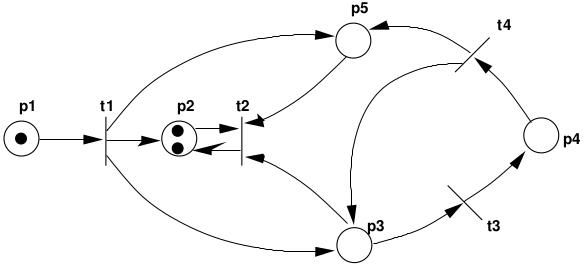
\includegraphics[width=0.975\linewidth]{img/petri-net/mpn/marked-petri-net-example.png}
    \end{minipage}%
    \begin{minipage}[t]{.5\textwidth}
      \centering
      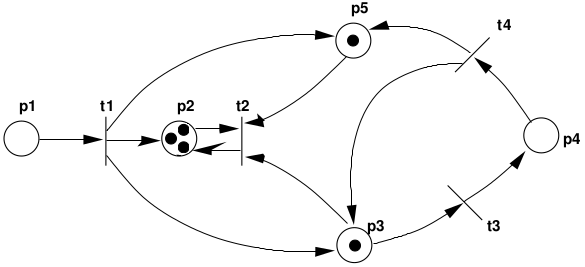
\includegraphics[width=0.975\linewidth]{img/petri-net/mpn/marked-petri-net-after-t1-firing-example.png}
    \end{minipage}
    \caption{Evolution of a Marked Petri Net after firing of transition $t_1$.}
    \label{fig:marked-petri-net-transition-firing-example}
\end{figure}

\

Two enabled transitions conflict when the act of firing one prevents the firing in the other.
If two transitions are enabled, both can be fired, but not simultaneously.
The flexibility provided with the properties of non-determinism and no simultaneous firing of transitions allows concurrency (Figure \ref{fig:marked-petri-net-concurrency}) and conflicts (Figure \ref{fig:marked-petri-net-conflict}) modeling.

\

\begin{figure}[h]
    \centering
    \begin{minipage}[t]{.45\textwidth}
      \centering
      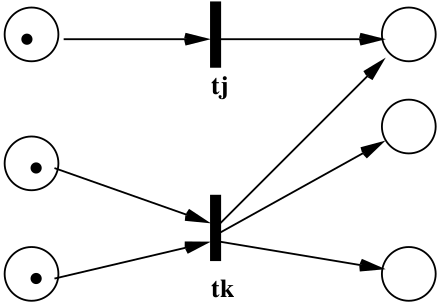
\includegraphics[width=0.725\linewidth]{img/petri-net/mpn/marked-petri-net-concurrency.png}
      \caption{Concurrency modelling with two possible execution sequences, $t_j t_k$ or $t_k t_j$ \cite{lecture-notes-concurrent-systems-validation}.}
      \label{fig:marked-petri-net-concurrency}
    \end{minipage}
    \hspace{0.3cm}
    \begin{minipage}[t]{.45\textwidth}
      \centering
      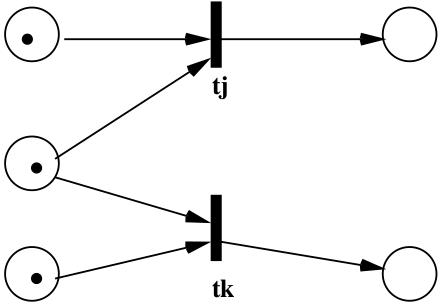
\includegraphics[width=0.725\linewidth]{img/petri-net/mpn/conflict/marked-petri-net-conflict.png}
      \caption{Conflict modelling, either $t_j$ or $t_k$ can be fired \cite{lecture-notes-concurrent-systems-validation}.}
      \label{fig:marked-petri-net-conflict}
    \end{minipage}
\end{figure}

A marking $M'$ is immediately reachable from an initial marking $M$ if and only if an enabled transition can be fired resulting in $M'$.
$M'$ is reachable from $M$ if there is a sequence of fired transitions from $M$ resulting in $M'$.
Of course, if a marking is immediately reachable, it is also reachable.


\subsection{Petri Nets properties}
Given a Marked Petri Net $R=(P,\ T,\ I,\ O,\ M_0)$, then one property of its places is k-limitation. A place is k-limited for an initial marking $M_0$ when 
$$ \exists k\in\mathbb{N} \ : \ M'(p_i) \leq k \hspace{0.5cm} \forall M' \in \mathcal{M}(R, M_0).$$

This property can be extended to the whole net.

\

\definition{K-limited Marked Petri Net.}{ A Net is called k-limited for the initial marking $M_0$ if and only if all its places are k-limited for that initial marking.}

\

If the Net is k-limited for any $k\in\mathbb{N}$, then the reachability set is finite.

\

\definition{Secure Net.}{ A 1-limited Net.}

\

\definition{Structurally limited Marked Petri Net.}{ It is a special kind of Net limited for all the possible initial finite marking.}

\

Another interesting property is liveness.
liveness will be defined for transitions and then generalized to the entire Net.

\

\definition{Alive transition.}{ A transition $t\in T$ is alive when for all the markings in the reachability set of the Net, there is a sequence of firings that will enable the transition $t$. Formally,
$$\forall M\in \mathcal{M}(R, M_0)
\hspace{0.3cm} \exists \sigma : M\rightarrow M'
\hspace{0.3cm} \text{ such that }
\hspace{0.3cm} t\in \sigma.$$}

liveness ensures that no transition firing sequence will block a transition, preventing it to be potentially enabled again. This property can be generalized:

\

\definition{Alive Marked Petri Net}{ for the initial marking $M_0$ when all the transitions are alive for that initial marking.}

\

Liveness can be relaxed to include more Nets when an initial marking to make the Net alive exists.

\

\definition{Structurally alive Marked Petri Net}{ is a Net allowing an initial finite marking $M_0$ where the Net is alive.}

\

The alive property is more general.
The relationship between these two liveness properties is shown in Figure \ref{fig:mpn-liveness-property-summary}.

\

\begin{figure}[H]
    \centering
    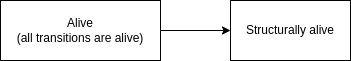
\includegraphics[scale=0.675]{img/petri-net/mpn/property/mpn-liveness-properties-summary.png}
    \caption{Liveness properties relationship for Marked Petri Nets \cite{lecture-notes-concurrent-systems-validation}.}
    \label{fig:mpn-liveness-property-summary}
\end{figure}

\

A Marked Petri Net is \textbf{cyclic} for the initial marking $M_0$ when there is a transition firing sequence reaching again $M_0$ for any reachable marking:
$$\forall M\in \mathcal{M}(R, M_0) \hspace{0.5cm} \exists\sigma : M \rightarrow M_0.$$

From the concurrency point of view, it is critical to categorize the conflicts to find better ways to represent them.
There are two kinds of conflicts, structural and effective. 

\

\definition{Structural conflict (Figure \ref{fig:marked-petri-net-structural-conflict}).}{ It occurs when a place $p\in P$ is linked with more than one output transition, but these output transitions can not be simultaneously enabled for any reachable marking.}

\

\definition{Effective conflict between two transitions $t_1,t_2\in T$ (Figure \ref{fig:marked-petri-net-effective-conflict})}{ for an initial marking $M_0$ if there is a potential marking $M\in \mathcal{M}(R, M_0)$ that will enable both transitions, and, after firing one of them, the other will lose its enabled status.}

\

\begin{figure}[h]
    \centering
    \begin{minipage}[t]{.45\textwidth}
      \centering
      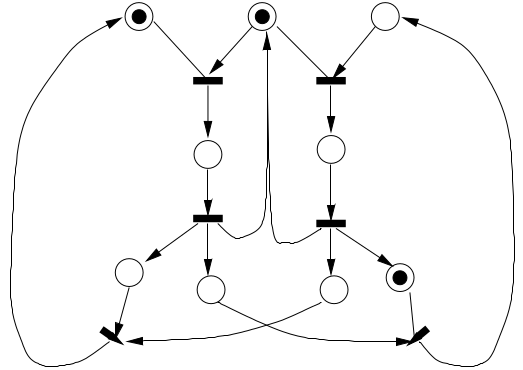
\includegraphics[width=0.85\linewidth]{img/petri-net/mpn/conflict/mpn_with_structural_conflict.png}
      \caption{Structural conflict, it is not possible to have the three upper places simultaneously marked \cite{lecture-notes-concurrent-systems-validation}.}
      \label{fig:marked-petri-net-structural-conflict}
    \end{minipage}
    \hspace{0.25cm}
    \begin{minipage}[t]{.45\textwidth}
      \centering
      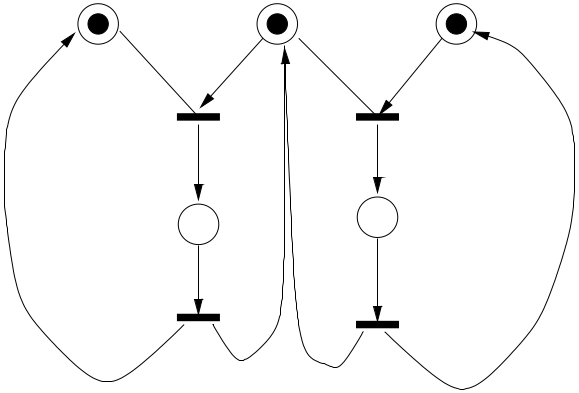
\includegraphics[width=0.85\linewidth]{img/petri-net/mpn/conflict/mpn_with_effective_conflict.png}
      \caption{Effective conflict between the two upper transitions \cite{lecture-notes-concurrent-systems-validation}.}
      \label{fig:marked-petri-net-effective-conflict}
    \end{minipage}
    % TODO?: simplify both nets
\end{figure}

Both definitions rely on the initial marking of the Net since they depend on the reachable markings.
As a consequence of the definitions, the intersection of the structural conflicts and effective conflicts is empty.
It is possible to model the resources of a system using the markings.
For these scenarios, it is relevant to distinguish Nets where resources are created/destroyed/kept.

\

\definition{Strictly conservative Marked Petri Net}{, a given Net $R=(P,\ T,\ I,\ O,\ M_0)$ verifying that the total amount of marks is constant
$$\forall M'\in\mathcal{M}(R, M_0),\hspace{0.3cm} \sum_{p_i\in P} M'(p_i) = \sum_{p_i\in P} M(p_i).$$}

\

From the strictly conservative property follows that no transition can reduce or increment the number of marks on the Net.
That behaviour would produce a marking with a different amount of marks than the initial one.
As a consequence, for all the potentially enabled transitions $t_j\in T$ the property $|I(t_j)| = |O(t_j)|$ is verified.
There is also a relaxed conservative property:

\

\definition{Conservative Marked Petri Net}{, a given Net $R$ where, for specific weights in the places, $w=(w_1, ..., w_n)$, the weighted sum of the markings is constant:
$$\forall M' \in \mathcal{M}(R, M_0),\hspace{0.5cm} \sum_{p_i\in P} w_i \cdot M(p_i) = \sum_{p_i\in P} w_i \cdot M('p_i).$$
}
% TODO?: include example of conservative MPN that it is not strictly conservative

\

\definition{Repetitive MPN.} { It is a Marked Petri Net containing a transition sequence including all the transitions. That sequence must finish in the same initial marking, like:
$$M \overset{\sigma}{\longrightarrow} M\hspace{1cm} \wedge \hspace{1cm}\forall t\in T,\hspace{0.3cm} t\in\sigma \hspace{1cm} M\in \mathcal{M}(R, M_0).$$}

\

Finally, the security properties summary appears in Figure \ref{fig:mpn-security-property-summary}.

\

\begin{figure}[H]
    \centering
    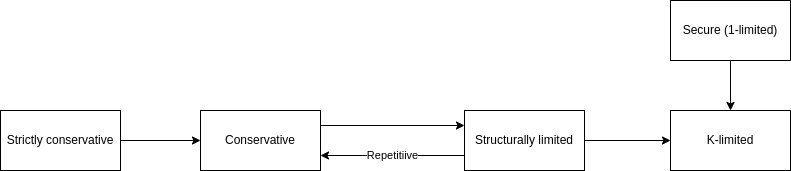
\includegraphics[scale=0.6]{img/petri-net/mpn/property/mpn-security-properties-summary.png}
    \caption{Security properties relationship for Marked Petri Nets \cite{lecture-notes-concurrent-systems-validation}.
    The implication from structurally limited to conservative when the net is repetitive is not proven.}
    \label{fig:mpn-security-property-summary}
\end{figure}


The next section presents an algorithmic approach for studying the possible markings of a net.

\

\subsection{Reachability tree generation}
Most of the described properties depend on the reachability tree.
The reachability problem consists of, given a specific marking in a Petri Net, verifying if the marking belongs to $\mathcal{M}(R, M_0)$ or not.
Each node is a marking on the Net, represented as a vector whose i-component is the number of marks for the place $p_i$ on the Net, i.e. $$(M(p_1),\ M(p_2),\ ...\ ,\ M(p_n)) \hspace{1cm} p_1,\ p_2,\ ...,\ p_n\in P.$$
It is possible to define a partial order relationship between two markings $M_1 = (a_1, ..., a_n),\ M_2 = (b_1, ..., b_n)$ such that
$$M_1 \leq M_2\hspace{0.5cm} \Longleftrightarrow \hspace{0.5cm} \forall i\in \{1, ..., n\} : a_i \leq b_i,$$
\begin{equation}
\label{eqn:mpn-order-relationship}
M_1 < M_2\hspace{0.5cm} \Longleftrightarrow \hspace{0.5cm} M_1 \leq M_2 \ \wedge \ \exists i\in \{1, ..., n\} : a_i < b_i.
\end{equation}

\

The algorithm to compute the finite reachability tree uses a symbol $\omega$ to represent the infinite, and there is no change in that value if there is a sum or subtraction.

\

\procedure{Reachability tree generation}{
\begin{itemize}
    \item Starts from the initial marking $M_0$.
    \item Each enabled transition will generate a node (unless that node is already in the tree).
    \item After the creation of the next node $M_j$, if there is another node in the tree $M_i$, such that,
    $$M_j \in \mathcal{M}(R, M_i) \hspace{0.4cm} \wedge \hspace{0.4cm} M_j \geq M_i,$$
    then all the places where $M_j$ has more marks than $M_i$ are marked with $\omega$.
\end{itemize}}

\

Example of the computation of a reachability tree:

\begin{figure}[H]
    \centering
    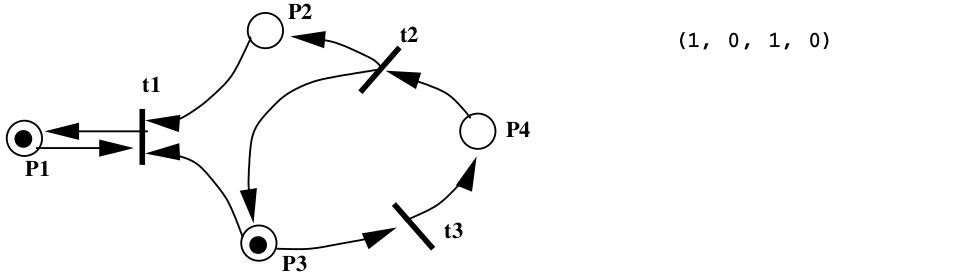
\includegraphics[scale=0.45]{img/petri-net/reachability-tree-example/reachability-tree-step1.png}
\end{figure}
The first step of the tree represents the initial marking $(M(p_1),\ M(p_2),\ M(p_3),\ M(p_4))$.

\begin{figure}[H]
    \centering
    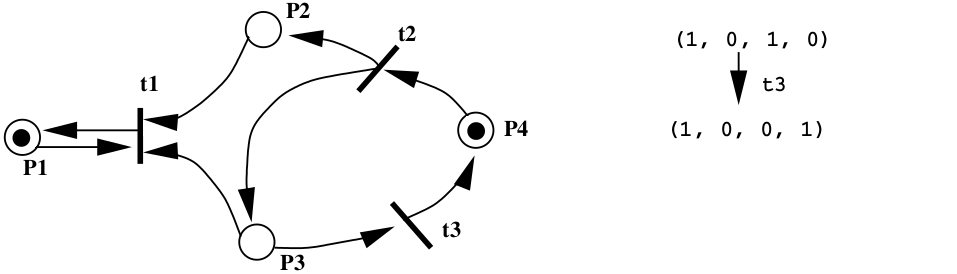
\includegraphics[scale=0.45]{img/petri-net/reachability-tree-example/reachability-tree-step2.png}
\end{figure}

After firing of the only enabled transition ($t_3$), it shifts the mark $p_3$ to $p_4$.

\begin{figure}[H]
    \centering
    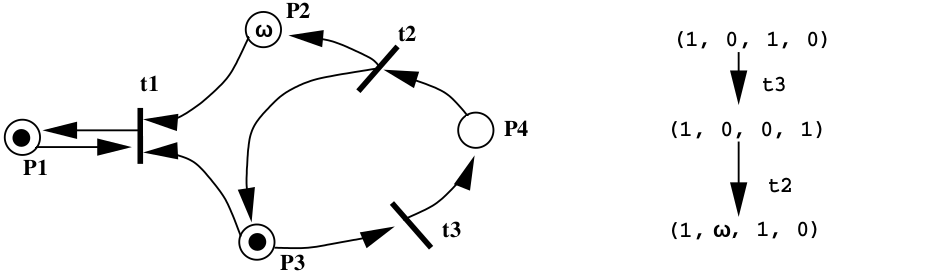
\includegraphics[scale=0.475]{img/petri-net/reachability-tree-example/reachability-tree-step3.png}
\end{figure}
Firing of $t_2$ removes mark from $p_4$ and generate marks in $p_2$ and $p_3$.
This Net is \textbf{not conservative} since the total number of marks is potentially infinite.
There is no combination of weights keeping the weighted sum of marks constant.
Notice that this marking is reachable from the initial marking and greater than it (using (\ref{eqn:mpn-order-relationship})).
The set of places with more marks now than in the initial marking is $\{p_2\}$.
Then, the number of marks in $p_2$ is replaced with $\omega$.
Without the $\omega$ rule, another sequence of transition firings ($t_1,t_2$) would produce another node.
To avoid infinite nodes in the reachability tree, the infinite sequence of nodes
$$\{(1,1,1,0),\ (1,2,1,0),\ ...,\ (1,n,1,0),\ (1,n+1,1,0),\ ...\}$$
is simplified to $(1,\omega,1,0)$ allowing the algorithm to be finite for any Net.
\textbf{When there is any $\omega$ in the reachability tree the Net is not k-limited} for any $k\in\mathbb{N}$, therefore is not a secure Net.
Now, it is clear that a node does not strictly represent a marking, but a equivalence relation between comparable markings.

\begin{figure}[H]
    \centering
    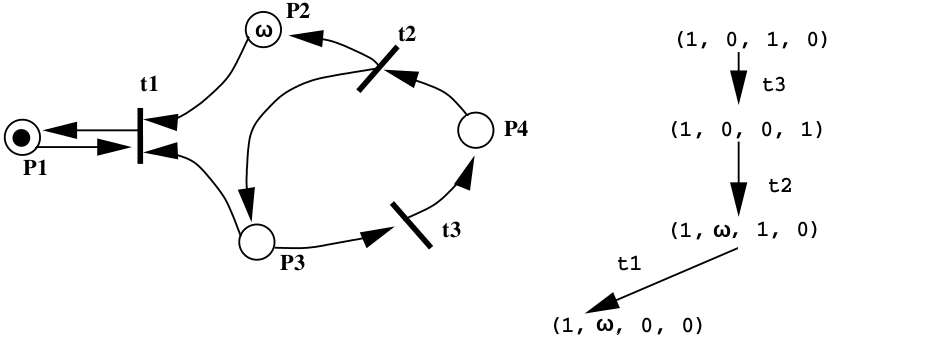
\includegraphics[scale=0.45]{img/petri-net/reachability-tree-example/reachability-tree-step4.png}
\end{figure}
Now, all the inputs for transition $t_1$ have marks (indeed, $p_2$ has potentially infinite marks).
Both, $t_1$ and $t_3$, are enabled now.
After firing of $t_1$ the mark in $p_3$ disappears but $p_2$ still has $\omega$ marks.
After this firing, $t_1$ is no longer an alive transition.
Indeed, no transition is potentially enabled again, and \textbf{the liveness property is not verified}.

\begin{figure}[H]
    \centering
    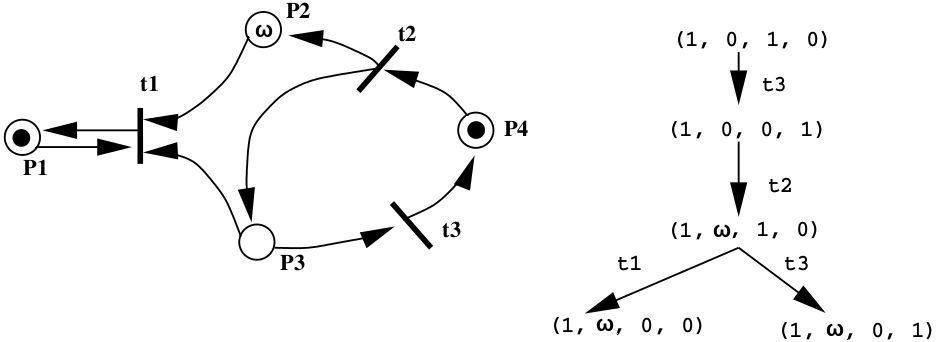
\includegraphics[scale=0.45]{img/petri-net/reachability-tree-example/reachability-tree-step5.png}
\end{figure}
If instead of $t_1$, $t_3$ is fired then there is another node in the tree.

\begin{figure}[H]
    \centering
    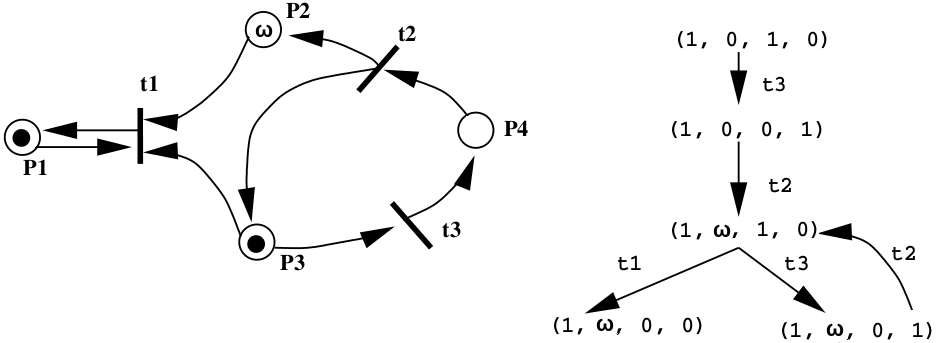
\includegraphics[scale=0.45]{img/petri-net/reachability-tree-example/reachability-tree-stepn.png}
    \caption{Final reachability tree generation.}
    \label{fig:reachability-tree-stepn}
\end{figure}
The only missing enabled transition is $t_2$, after that, there is no node to explore and the final reachability tree is shown in Figure \ref{fig:reachability-tree-stepn}.

\ 

In the example above, the Net is not alive because a node in the tree did not have any available transition.
As it turns out, if the reachability tree has any leaf node, then the Net is not alive.
The tree can be adapted to create an algorithm to check the liveness property.
The transition firings will now be nodes, and the marking relationships will be edges.
In the transformed tree, all the nodes must be potentially reachable from any other node to verify the liveness property.
As a side note, if $\omega$ does not appear in the reachability tree, it is possible to check limited and conservative properties using the generated tree \cite{lecture-notes-concurrent-systems-validation}.

\

It is the moment to introduce some static properties that do not depend on the initial or current marking of a net.
They are called invariant properties.
It is possible to prove some Petri Nets properties using matrix operations \cite{lecture-notes-concurrent-systems-validation}.
Using the number of arcs between a place and a transition, it is possible to define two matrices:
$$D^-[j,i] := n(p_i, I(t_j)), \hspace{1.5cm} D^+[j,i] := n(p_i, O(t_j))\hspace{1cm} j\in\{1,...,|T|\},\ i\in\{1,...,|P|\}.$$
The dimension of the matrix is $|T| \times |P|$.
It could not be a square matrix since the number of places could differ from the number of transitions.

\

\definition{Incidence Matrix}{, defined as
$$D := D^- - D^+ \hspace{1cm} D^-,D^+\in M_{|T| \times |P|} (\mathbb{N_0^+}).$$}

\

The only remarkable ambiguity is that zeros in $D$ could mean either no link (pure nets) or an equal number of inputs and outputs.
As a consequence, the same matrix $D$ can represent different nets.
The next step is to define mathematically some of the previous Petri Net concepts.

\

\definition{Enabled transition}{. Given a transition $t_j$ and a vector $e_j = (0, ..., 1, ..., 0)_{1\times |T|}$ with all the elements zero except the jth, which is a one, then
$$t_j \text{ is enabled for the marking } M\hspace{0.5cm} \Longleftrightarrow \hspace{0.5cm} M \geq e_j \cdot D^-.$$}

\ 

\definition{Transition function}{, given a marking $M$ and a transition $t_j$, the generated marking of the net after $t_j$ firing is:
$$\delta (M,t_j) := M - e_j\cdot D^- + e_j\cdot D^+.$$}

\

The incidence matrix simplifies the study of the transitions of a Petri Net because it allows us to use only one matrix from now on.
Following the definitions of the incidence matrix and the transition function, it is possible to deduce the next corollary without formal proof.

\

\corollary{$\delta(M, t_j) = M + e_j\cdot D.$}

\

For a finite list of transitions $t_a, t_b, ... \in T$ it is possible to generalize the transition function using $\sigma = {t_a, t_b, ...}$,
$$\delta(M, \sigma) \ =\ M + (e_a + e_b + ...) \cdot D \ =\ M + f(\sigma) \cdot D.$$
$f(\sigma)$ represents the firing vector and its value at index $i$ represents the number of firings of transition $t_i$.
Now it is possible to define the state equation:

\

\definition{Petri Net state equation}{ for a given initial marking $M_0$:
$$M' = M_0 + f(\sigma) \cdot D.$$}

\

Having a formal description of the evolution of the markings of a net it is not possible to assume that any mark combination is possible.
The notation for the possible firing sequences is defined in the next corollary.

\

\corollary{Not every firing sequence combination is valid.
The valid sequences are
$$L(R, M_0) := \{ \sigma \ | \ M_0 \overset{\sigma}{\longrightarrow} M \} \subset T^{\mathbb{N}}.$$}

\

\corollary{$\sigma$ does not fix any order, different sequence orders could lead to the same $f(\sigma)$.
That's why it is not possible to infer a sufficient vivacity condition with this notation.}

% TODO? Definición 4.15, Proposición 4.1, Proposición 4.2, Proposición 4.3

\

The reachability problem is equivalent to the existence of a solution $X$ verifying
$$M' = M + X\cdot D \hspace{1cm} X\in L(R, M).$$

\


\proposition{ Given a Petri Net $M$ with incidence matrix $D$, then
$$\exists Y\in (\mathbb{N}^+)^{|T|}\ /\ D_{|T|\times |P|} \cdot Y^T_{|P|\times 1} = 0\hspace{0.5cm} \Longleftrightarrow \hspace{0.5cm} M \text{ is conservative.} $$}{
$ $\newline
$\Longrightarrow$\newline
From the state equation,
$$M' = M +X\cdot D
\hspace{0.3cm}
\Longrightarrow
\hspace{0.3cm}
M'\cdot Y = M\cdot Y + X\cdot D\cdot Y \hspace{0.15cm}
\overset{(\ast)}{\implies}
\hspace{0.3cm}
M'\cdot Y = M\cdot Y.$$
Where $(\ast)$ means the precondition ($D_{|T|\times |P|}\cdot Y^T_{|P|\times 1} = 0$).
$Y$ is composed of positive natural numbers, so one firing verifies the assertion.
A reachable marking is a finite sequence of firings.
As a result, the Petri Net $M$ is conservative. \newline\newline
$\Longleftarrow$
$$\forall M' \in \mathcal{M}(R, M_0),\hspace{0.5cm} \sum_{p_i\in P} w_i \cdot M(p_i) = \sum_{p_i\in P} w_i \cdot M('p_i)\hspace{0.5cm} w_i>0 \hspace{0.4cm} \forall i\in\{1,...,w_{|P|}\},$$
then, $Y = (w_1,...,w_{|P|}) \in (\mathbb{N}^+)^{|P|}$.
Again, from the state equation.
$$M' = M +X\cdot D
\hspace{0.3cm} \Longrightarrow
\hspace{0.3cm} M'\cdot Y = M\cdot Y + X\cdot D\cdot Y
\hspace{0.3cm} \overset{(\ast)}{\implies} \hspace{0.3cm}
0 = X\cdot D\cdot Y.$$
Where $(\ast)$ comes from the conservative condition ($M'\cdot Y = M\cdot Y$).
$X$ can not be zero because it is a non-empty sum of elements $e_i$ of the standard basis. In conclusion, $D\cdot Y=0$.}

\

\definition{Marking invariant}{, property verified for all reachable markings from a starting one.}

\

In conservative Petri Nets, the invariants do not depend on the initial or current marking and derive from the proven condition.
These invariants are vectors $Y_i$ from the system $D\cdot Y^T = 0$, having $|P|$ equations and $|T|$ unknown values.
In general, there are no restrictions for the elements of each vector $Y_i$.
Defining
$$r := range(D) \hspace{0.5cm} 0\leq r \leq \min(|P|, |T|),$$
if $(|P| - r) > 0$ we have a linear span
$$B 
= \{Y_i \ / \ Y_i
= (Y_{i,1}, ..., Y_{i,|P|}),\ i\in\{1, ..., |P|-r\} , \ \ Y_{i,j}\in\mathbb{Z}\}.$$

$B$ is called the system of right overridjes for the incidence matrix $D$, and any solution for $D\cdot Y^T = 0$ is a linear combination of vectors from $B$.
Since all the vectors from $B$ must verify the invariant property, then this restriction is also required:
$$M\cdot B = M_0\cdot B \hspace{0.5cm}M\in\mathbb{N}^{|P|}.$$
It is possible to verify that a marking is not reachable by checking all these conditions.

\

\definition{Conservative component}{ of a Petri Net with incidence matrix $D$ is each vector $Y\in\mathbb{N}^{|P|}$ such that $D\cdot Y^T = 0$.}

\

\definition{Support of a conservative component}{ $Y$ is the set of places associated with non-zero elements of $Y$, denoted as $\|Y\|$.}

\

The producer-consumer is a known concurrency problem.
It models the data flow between two different processes, one producer and one consumer.
Producer continuously creates data and sent to a common buffer, where the consumer can consume data at its own pace.
There are many variants, with several producers/consumers/buffers.
In its simpler version, one producer creates data and send it to one buffer, while only one consumer use the data in the buffer.
Marked Petri Nets can model a network representing the producer-consumer problem, as shown in Figure \ref{fig:mpn-producer–consumer}.
In the figure, there are three producers (not completely independent since they are connected to each other), represented as three subgraphs,
$$\{\{p_1, p_2 \},\ \{p_5, p_6\},\ \{p_3, p_4 \}\}.$$
There are two buffers ($\{t_2, t_3\}$), and the consumers are the same than the producers, the three subgraphs.
The firing of fork transitions like $t_2,\ t_3$ produces two marks in the graph and removes just one.
There is no way to reduce the number of marks since there is no joint transition.
In conclusion, the net represented in Figure \ref{fig:mpn-producer–consumer} is not secure because it is not 1-limited.



\

\begin{figure}[H]
    \centering
    \includegraphics[width=0.5\linewidth]{img/petri-net/mpn/mpn-producer–consumer.png}
    \caption{Producer-consumer with conservative components $\{\{p_1,\ p_2\}, \{p_5,\ p_6\}, \{p_3,\ p_4\}\}$}
    \label{fig:mpn-producer–consumer}
\end{figure}

It is easy to identify that the conservative components from Figure \ref{fig:mpn-producer–consumer} represent different substructures in the Petri Net, joined by transitions $t_2,t_3$.
The computation of its conservative invariants derives from:
$$D\cdot Y^T = 0 \implies
    \begin{pmatrix}
        -1 &  1 &  0 &  0 &  0 &  0 \\
         1 & -1 &  0 &  0 & -1 &  1 \\
         0 &  0 & -1 &  1 &  1 & -1 \\
         0 &  0 &  1 & -1 &  0 &  0
    \end{pmatrix}
    \cdot
    \begin{pmatrix}
        y_1 \\ y_2 \\ y_3 \\ y_4\\ y_5 \\ y_6
    \end{pmatrix}
    = 0.$$

\

\definition{Fundamental conservative component set}{ is the linear span
$\mathcal{Y} := \{Y_1,\ ... \ ,\ Y_n\}$
with fewer elements able to generate any conservative component.
$$Y = \sum_{Y_i\in\mathcal{Y}} k_i\cdot Y_i \hspace{1cm} k_i\in\mathbb{N}_0^+,$$
and the elements $Y_i$ are called elemental components.}

\

This fundamental set is finite and unique \cite{lecture-notes-concurrent-systems-validation}.
Each elemental component represents a restriction in the evolution of the marks.
A previous section presented the concepts of structural and effective conflicts.
Now we provide a sufficient condition to verify that two places can not be enabled simultaneously.

\

\proposition{\textbf{Mutual exclusion between two places}.
Given a conservative component $Y$, and two places in its support, $p_i,p_j\in\|Y\|$, then
$$Y(p_i) + Y(p_j) > M_0\cdot Y \hspace{0.3cm}\implies\hspace{0.3cm}p_i,p_j\ \text{ can not be simultaneously enabled.}$$} {
Using the invariant relationship for a given marking $M\in\mathcal{M}(R, M_0)$:
$$M_0\cdot Y 
= \sum_{p_k\in P} M(p_k) \cdot Y(p_k)
\ \geq \ M(p_i) \cdot Y(p_i) + M(p_j) \cdot Y(p_j).$$
If both $M(p_1), M(p_j)\not = 0$, using the precondition of the proposition there is a contradiction.
Then, either $M(p_i)=0$ or $M(p_j)=0$ for all the reachable markings, since there was no other restriction choosing $M$.}

\

The analysis of the invariants uses markings independent of the specific firing order.
Several firing orders can end with the same marking.
This limitation prevents the existence of a sufficient condition for Petri Net liveness in terms of its invariants.
It is possible to avoid this limitation using reachability tree analysis.
As we saw previously, if the reachability tree contains any leaf node, the net is not alive.
Tree search algorithms can determine the liveness property of a Net.


% TODO?: algorithm in the reachability tree to verify liveness.

\

The next section will show an extension of the Marked Petri Nets which will allow simplifying the representation of some complex models.

\

\subsection{Colored Petri Nets}
With the objective of having simpler descriptions of complex systems, a new type of Petri Net is introduced, Colored Petri Nets \cite{lecture-notes-concurrent-systems-validation}.
They will be used as a modeling language with the capability to analyze complex systems more easily than using Marked Petri Nets.
In particular, a subset of them are studied in this project, Well-formed Nets:
$$\text{Well-formed Nets} \hspace{0.3cm} \subset  \hspace{0.3cm} \text{Colored Petri Nets}  \hspace{0.3cm} \subset  \hspace{0.3cm} \text{High Level Petri Nets}$$
Intuitively, in Colored Petri Nets, it is possible to have different mark types, each with a different color.
These colors do not need to be the same in all the places.
Each place can define a different color domain.
If the color domain is finite, it is possible to transform the Color Petri Net into simpler Nets without colors using an unfolding procedure.
If the firing of the output transitions of a place does not depend on the colors, the colors can be viewed as a way to distinguish information (i.e. each color represents the firing from a different transition) but they don't increase the expressiveness of Marked Petri Nets.

\

More information is required to represent different information flows.
That's why the arcs between places and transitions (and only these, not the arcs between transitions and places) have annotations to restrict the marks that enable a transition.
More information is required to represent different information flows.
That's why the arcs between places and transitions (and only these, not from transitions to places) have annotations to restrict the marks that enable a transition.

\begin{figure}[H]
    \centering
    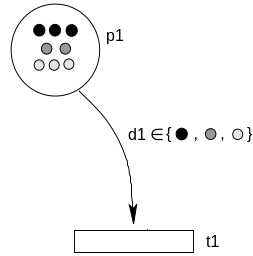
\includegraphics[width=0.275\linewidth]{img/petri-net/cpn/cpn-example.png}
    \caption{Colored Petri Net. Three different colors in place $p_1$, but only one ($d_i \in \{d_1, d_2, d_3\}$) enable transition $t_1$.}
    \label{fig:cpn-example}
\end{figure}

In Figure \ref{fig:cpn-example} a Colored Petri Net is shown. Marked Petri Nets can be generalized to include firing priorities, referencing different priorities drawing transitions with either boxes or lines.
For simplicity, there will be no consideration for priorities.
In the image, there is a label in the arc, $d_i$, belonging to the domain of possible colors for place $p_1$: $\{d_1, d_2, d_3\}$.
It is clear now that the marking definition must change to represent the distribution of colors in the marks, $M = \{m_1, m_2, m_3\}$.
In the image, there is a label in the arc, $d_i$, belonging to the domain of possible colors for place $p_1$: $\{d_1, d_2, d_3\}$.
It is clear now that the marking definition must change to represent the distribution of colors in the marks, $M = \{m_1, m_2, m_3\}$.

\

\definition{Colored Petri Net (CPN)}{ is 6-tuple $\mathcal{R} := (P,\ T,\ C^-,\ C^+,\ \mathcal{C},\ cd)$ verifying:
\begin{itemize}
    \item $P,\ T$ are non-empty finite disjoint sets representing the places and the transitions.
    \item $\mathcal{C}$ is the finite set of possible color classes for the marks.
    \item $cd: P \vee T \rightarrow \mathcal{C}$ defines the color domain for each place or transition.
    \item $C^- [p,t], \ C^+ [t, p]: cd(t) \rightarrow Bag(cd(p))$ are the transition matrices extending the definition of $D^-$ and $D^+$. Now the color must be taken into account in the matrix definitions.
    The $Bag$ function defines a multiset of colors, it is a set allowing several items of the same type.
    It allows for defining the matrices, specifying also the colors for each element.
\end{itemize}}

\

The incidence matrix definition is extended in Colored Petri Nets:
\begin{align*}
    C[p,t]    & : cd(t) \ \rightarrow \ Bag(cd(p)) \\
    C[p,t](x) & := C^+[t,p](x)\ -\ C^-[p,t](x).
\end{align*}
Not all the places and transitions need extra colors.
The neutral color is $C_{\bullet} = \{\bullet\}$.
If $\mathcal{C} = \{C_{\bullet}\}$ then the Color Petri Net can be simplified to a Marked Petri Net since
$$cd(p) = C_{\bullet} \hspace{0.5cm}\forall p\in P
\hspace{1cm} \wedge \hspace{1cm} 
cd(t) = C_{\bullet} \hspace{0.5cm}\forall t\in T$$

Previously, the marking of a place was represented with a number. Now, the definition must be generalized to include the distributions of color in the marks.

\

\definition{Marking in Colored Petri Net}{ is a vector $M := (M[p_1],...,M[p_n])$ representing the distribution of colors for each place.
Each element is a function
$$M[p_i] : cd(p_i) \rightarrow \mathbb{N}^+_0 \hspace{1cm} p_i\in P,$$
where $M[p_i,c] := M[p_i][c]$ represents the number of marks at place $p_i$ with color $c\in cd(p_i)$.}

\

\definition{CPN system}{ is a 2-tuple $<\mathcal{R},\ M_0>$
where $\mathcal{R}$ is a colored Petri Net and $M_0$ is a valid initial marking.}

\

CPN transition firings have increased granularity.
A transition $t\in T$ is enabled for a color, noted as
$$<t,c> \text{ is enabled }
\hspace{0.5cm}\Longleftrightarrow\hspace{0.5cm}
\forall p\in I(t) \hspace{0.3cm} M[p,c] \geq C^-[p,t](c)
\hspace{0.8cm} c\in cd(t) \subseteq \bigcap_{p_i \in I(t)} cd(p_i).
$$

The state equation is
$$M' := M + C[p, t](c) \hspace{1cm} p\in P,\ t\in T,\ c\in cd(t), \ M,M' \in \mathcal{M} (R, M_0).$$

The opportunity to include any amount of colors in a place dramatically expands the possible systems to make using a small amount of places/transitions.
The concept of the reachability tree is still the same, changing firing transitions with firings of the combinations of transition and colors.
In practice, even for small nets, this tree could be huge because a place/transition can handle any amount of colors, and each color would create a node in the tree.

\

Let's analyze Figure \ref{fig:cpn-user-input-clicks}.
It is a simplified version of the producer-consumer problem (also shown in Figure \ref{fig:mpn-producer–consumer}).
The producer would be the combination of $p_1$ and $t_1$, the buffer is $p_2$.
It could also be considered that $p_2$ is the consumer, it can store any amount of marks.
The transition $t_2$ creates two marks for each firing of $t_1$, one will go to $p_1$ and the other to $p_2$, the number of marks has no limit (there is no K-limitation there).
In this simplified model the power of Colored Petri Nets is not shown yet.
The model in Figure \ref{fig:cpn-user-input-clicks} can describe an infinite sequence of events, i.e. clicks from users without knowing the user that clicked.

\

\begin{figure}[H]
    \centering
    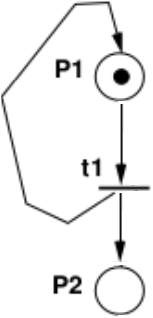
\includegraphics[scale=0.41]{img/petri-net/cpn/cpn-user-input-clicks.png}
    \caption{Modeling infinite user clicks (it is a simplified version of producer-consumer problem).}
    \label{fig:cpn-user-input-clicks}
\end{figure}

\

Colored Petri Nets would allow, for example, to represent a finite amount of users creating events (i.e. clicks), with the power to distinguish the origin using the color domain(s).
Another possibility is to expand the complexity of user input to better represent realistic real use cases.
Figure \ref{fig:cpn-user-input-choices} represents an infinite amount of user choices (true/false) thanks to the extra expressiveness of having two colors.
Now, the color domain would have two colors.
$$\mathcal{C} = \{c_1, c_2\} \hspace{1cm} cd(p_1) = cd(p_2) = cd(t_1) = \{c_1, c_2\} $$


\begin{figure}[H]
    \centering
    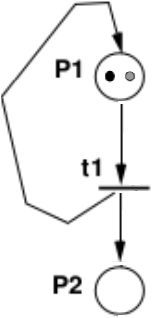
\includegraphics[scale=0.41]{img/petri-net/cpn/cpn-user-input-choices.png}
    \caption{Modeling infinite user choices (true/false).}
    \label{fig:cpn-user-input-choices}
\end{figure}

\

The generalization of the concept for storing any finite input form in Petri Nets is as follows.
Imagine a field in an online form to store the first name and then register a user in a system.
This kind of field usually has a maximum length (it does not make sense to allow first names with thousands of characters).
Hence, there is a finite amount of characters in the form.
A character encoding (i.e. UTF-8, Unicode, ...) represents each one of these characters.
Therefore, a character can be encapsulated in a finite amount of bits of information.
It turns out that this generalization extends to other types of data (numbers, etc.), in general, to any serializable object potentially sent in a fixed maximum amount of bits.
The representation is not straightforward, data abstraction(s) and set theory should be used to simplify the definitions for complex data types.

\


\begin{figure}[H]
    \centering
    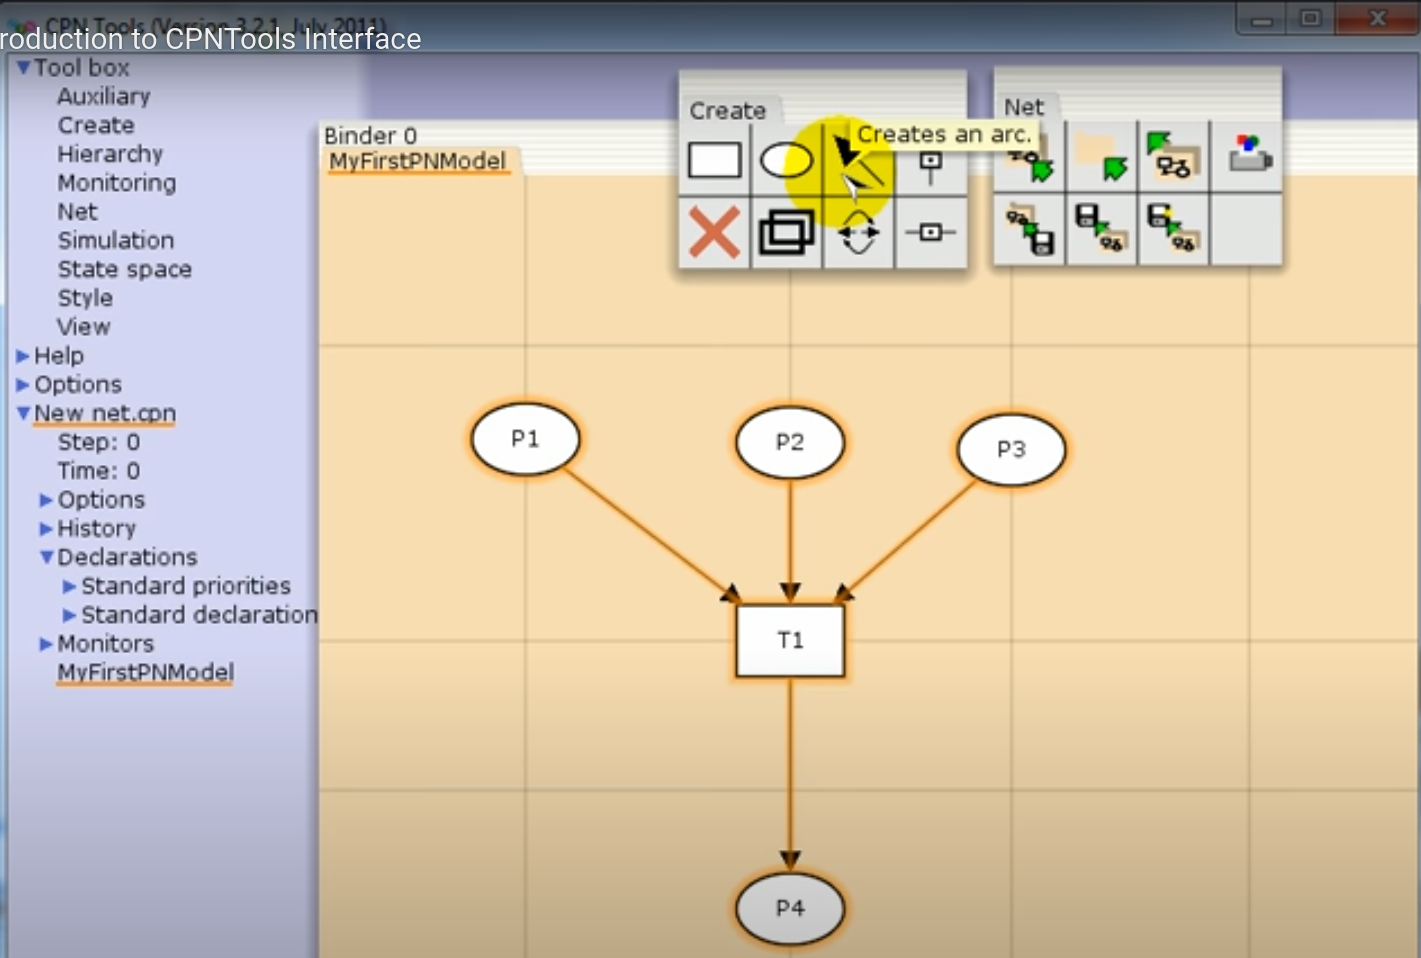
\includegraphics[scale=0.25]{img/petri-net/cpn-tools/examples/cpn-tools-create-net.png}
    \caption{Simplified CPN tools interface (from \cite{cpn-tools-tutorial-youtube}). Tool box for creating Colored Petri Nets.}
    \label{fig:cpn-tools-create-net}
\end{figure}

\


It is not optimal nor desirable to handle all these elements by hand.
To handle the increased complexity, CPN Tools are presented \cite{cpn-tools}, see Figure \ref{fig:cpn-tools-create-net}.
The origin of this tool is another tool (Design/CPN) from a research group from the University of Aarhus.
It is a WIMP (Windows, Icons, Menus, Pointer) graphical editor interface to model Colored Petri Nets and interact with them.
The first version dates from the year 2000 and requires OpenGL.
\cite{performance-analysis-cpn-tools}
CPN tools interface is shown in Figure \ref{fig:cpn-tools-create-net}.
Further references can be found in \textit{https://www.cpntools.org/}.



\newpage



\section{Multi-tenant Web Store implementation}
This general implementation of a multi-tenant web store will allow businesses to create a website with their products.
The most significant parts of the system are:

\begin{itemize}
    \item Admin Console: here, the proprietary of the platform MW-Store handles all the tenants (in our scenario, e-commerce) and the system users.
    See Figures \ref{fig:ecommerce-multi-tenancy-tenants} and \ref{fig:ecommerce-multi-tenancy-admins}.
    \item Tenant back office: administrators manage their e-commerce configuration using this interface. It is possible to handle the products and orders here.
    See Figures \ref{fig:ecommerce-multi-tenancy-admin-products} and \ref{fig:ecommerce-multi-tenancy-admin-orders}.
    \item User front end: the client will see the available products for the e-commerce where it is registered.
    An end-user can purchase in different e-commerces of the MW-Store if they have distinct accounts for each e-commerce.
    These final users will see their order history of purchased products.
    See Figures \ref{fig:ecommerce-multi-tenancy-products} and \ref{fig:ecommerce-multi-tenancy-orders}.
    \item Marketing site: potential MW-Store clients (businesses) will see an overview of a generated e-commerce with commercial purposes.
\end{itemize}

In MW-Store, all these components share an interface.
Each component is differentiated using automatic web URL redirection.
Data isolation between tenants is achieved using the DAO pattern with default tenant filtering.
The server sends a temporal encrypted tenant identifier from the back-end to the front-end stored in a JWT token generated after a valid login.
An HTTP interceptor in the front end sends the token in all the requests for proper tenant identification.
Sending another tenant in the request is equivalent to breaking the token encryption, fake user identifiers, and bypassing all the internal data consistency checks in the back-end.

\

The application verifies multi-tenancy properties.
The tenants, in this case, e-commerces, share the application context and the database, having a tenant identifier for each table.
The initial resource sharing approach is Shared Database, Shared Schema.
In the future, if the application grows enough and the load on one database is a bottleneck, a migration to a different approach would be considered.
No tenant has access to the data of other tenants by design, the front-end does not decide the tenant to query.
Different tenants have different redirections to differentiate one e-commerce from the other ones.
If a tenant, in some way, tries to use its credentials to access data from other tenants it will receive an error from the back-end.
The nature of this application is inherently concurrent and several properties will be formalized.


\subsection{Functional requirements}
First, let's discuss the structure of the system.
The root of the system is the super user.
This user has access privileges to the MW-Store admin console, where all tenants (Figure \ref{fig:ecommerce-multi-tenancy-tenants}) and their respective admins (Figure \ref{fig:ecommerce-multi-tenancy-admins}) are managed.

\

\begin{figure}[H]
    \centering
    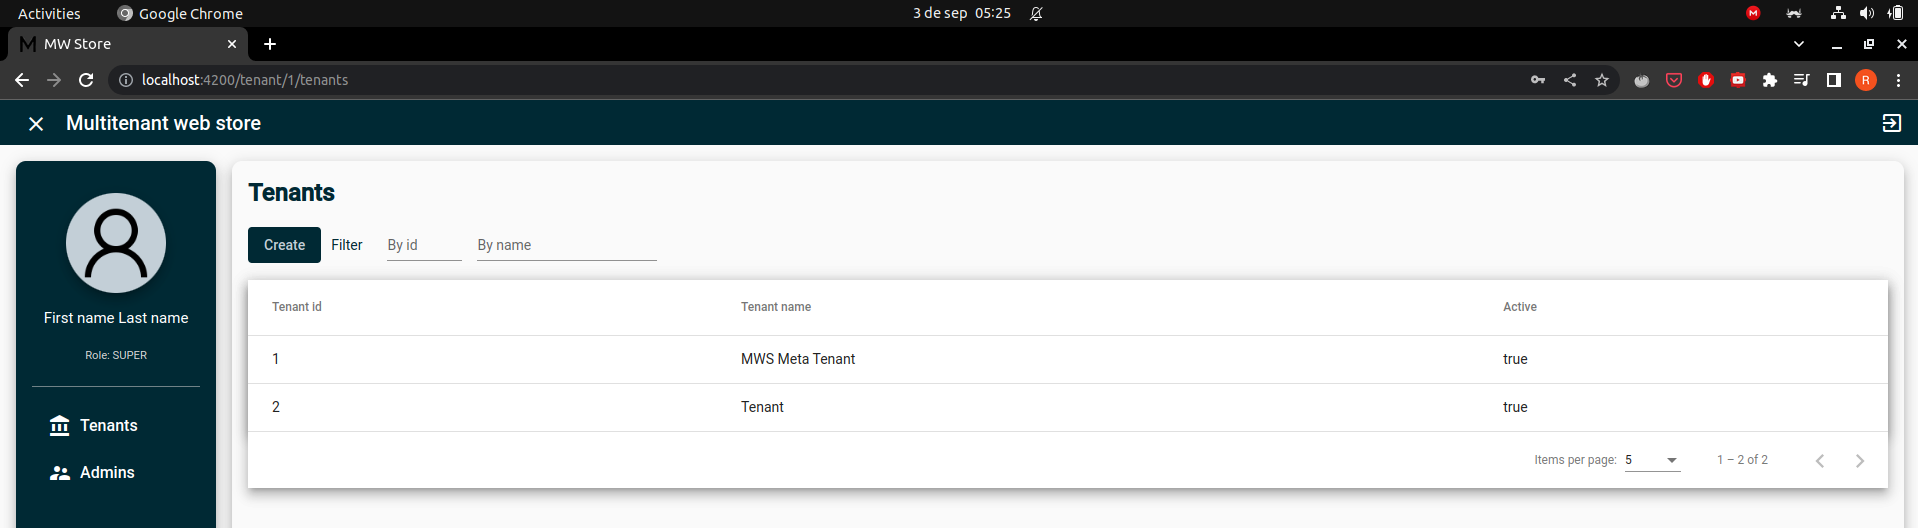
\includegraphics[scale=0.245]{img/mws/ecommerce-multi-tenancy-tenants.png}
    \caption{MW-Store admin console to manage tenants.}
    \label{fig:ecommerce-multi-tenancy-tenants}
\end{figure}

\begin{figure}[H]
    \centering
    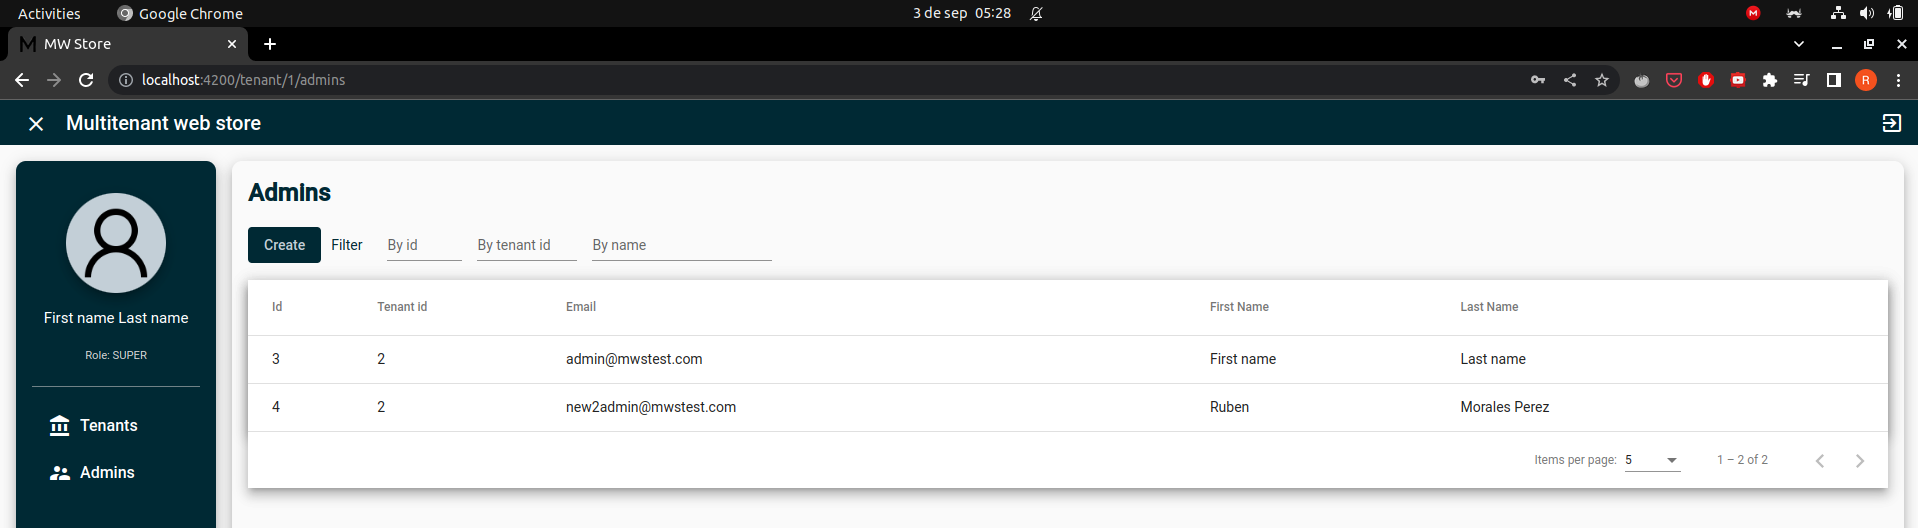
\includegraphics[scale=0.245]{img/mws/ecommerce-multi-tenancy-admins.png}
    \caption{MW-Store admin console to manage site admins.}
    \label{fig:ecommerce-multi-tenancy-admins}
\end{figure}

\

After the tenant and, at least, one admin for the tenant, products should be created.
The new admin has access to a back office with product management (Figure \ref{fig:ecommerce-multi-tenancy-admin-products}) and access to all the orders of the tenant (Figure \ref{fig:ecommerce-multi-tenancy-admin-orders}).

\


\begin{figure}[H]
    \centering
    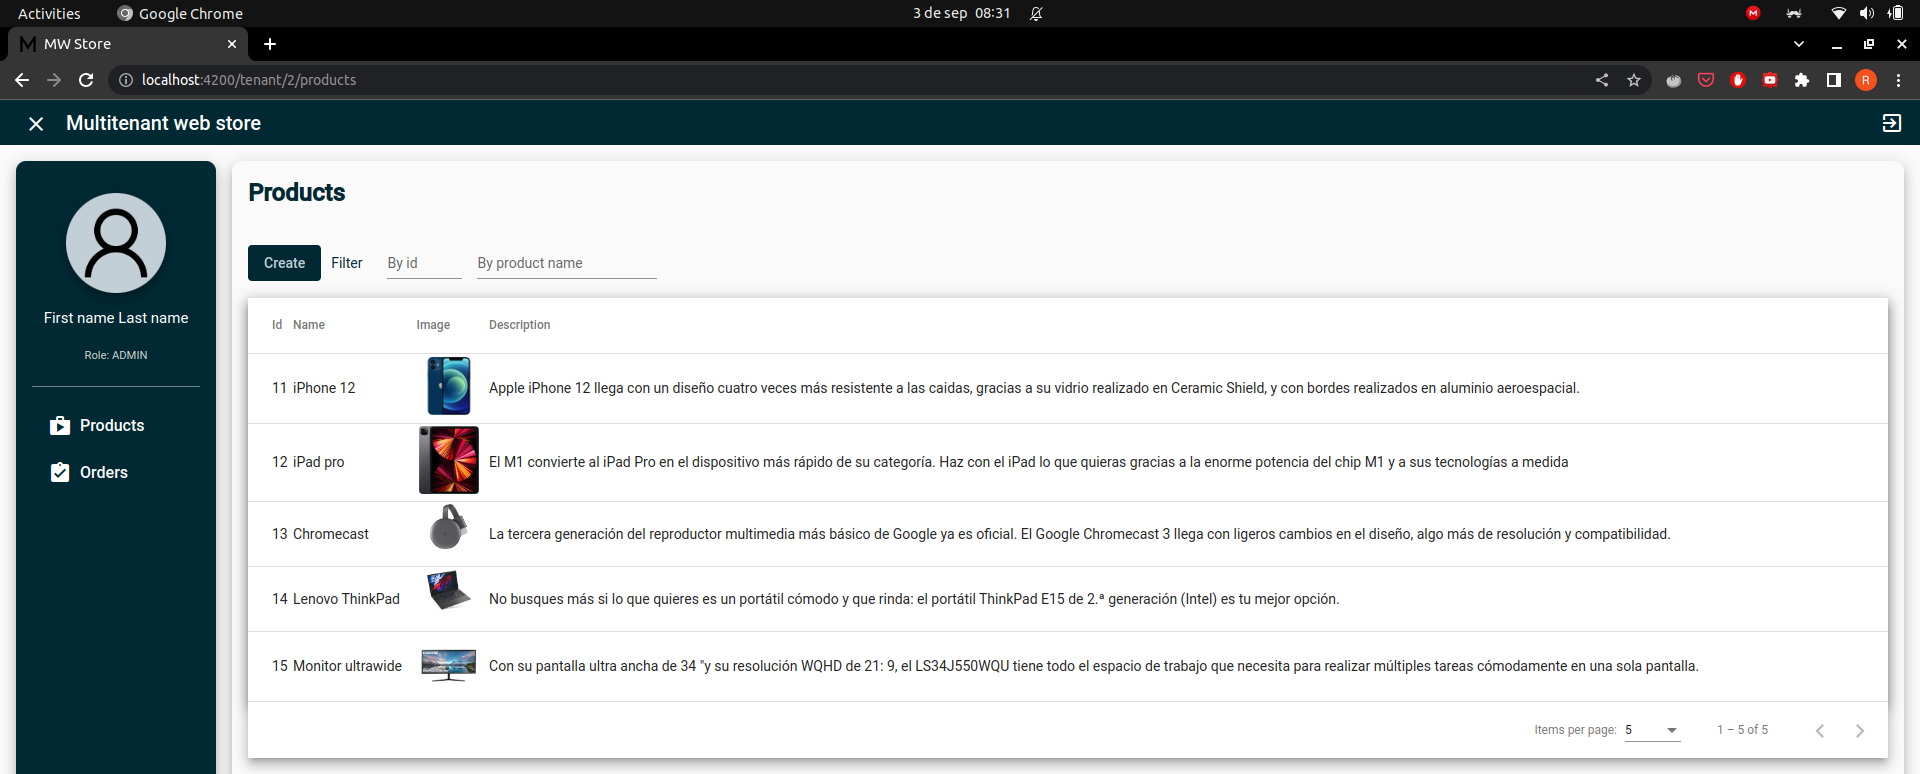
\includegraphics[scale=0.245]{img/mws/ecommerce-multi-tenancy-admin-products-management.png}
    \caption{Tenant admin back office. Products management interface.}
    \label{fig:ecommerce-multi-tenancy-admin-products}
\end{figure}

\begin{figure}[H]
    \centering
    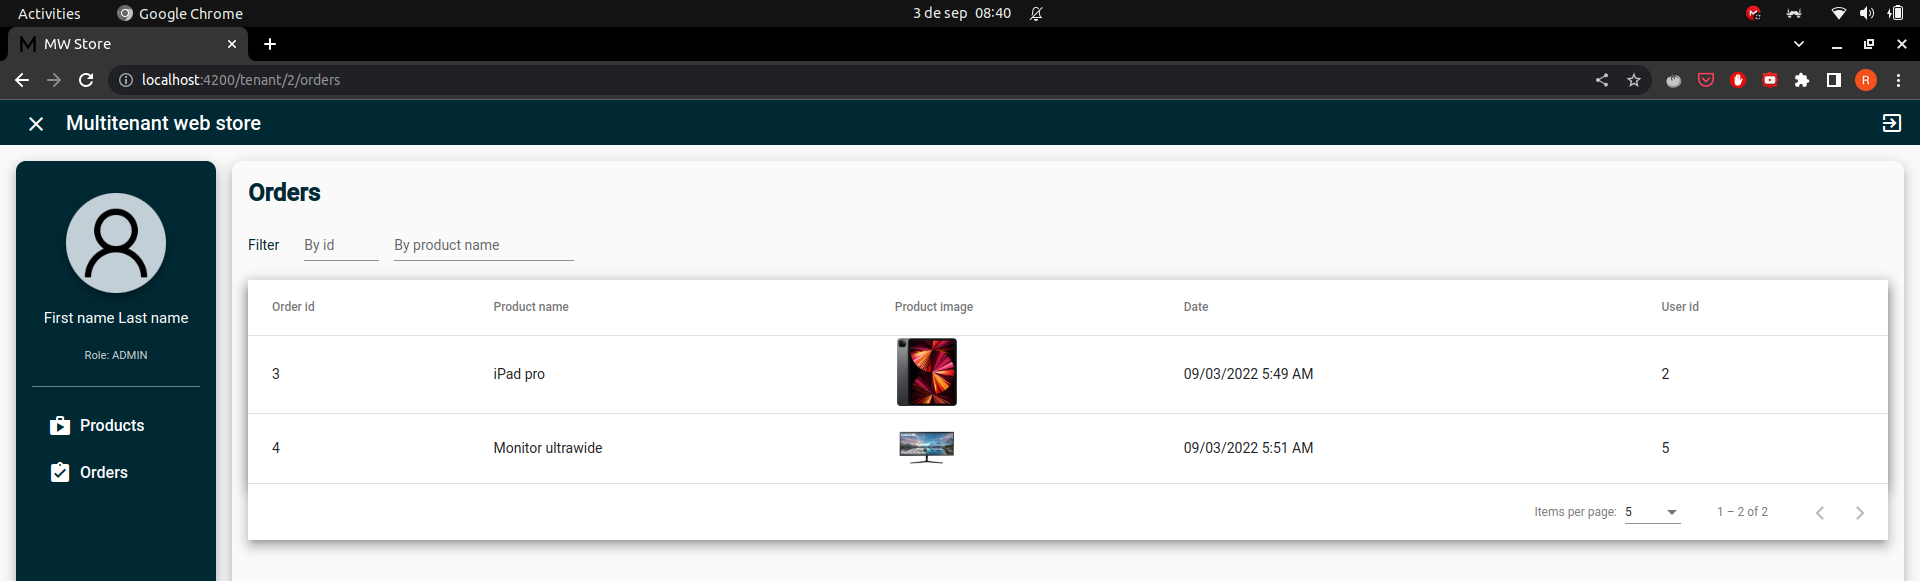
\includegraphics[scale=0.245]{img/mws/ecommerce-multi-tenancy-admin-orders-view.png}
    \caption{Tenant admin back office. Order management interface.}
    \label{fig:ecommerce-multi-tenancy-admin-orders}
\end{figure}


\ 

The designed system will store products, each one associated to a specific tenant.
Different tenants are allowed to create different products (Figure \ref{fig:ecommerce-multi-tenancy-products}) that will be bought by end users (Figure \ref{fig:ecommerce-multi-tenancy-orders}).
Each tenant is an organization and will handle their product(s) and keep track of the orders.

\begin{figure}[H]
    \centering
    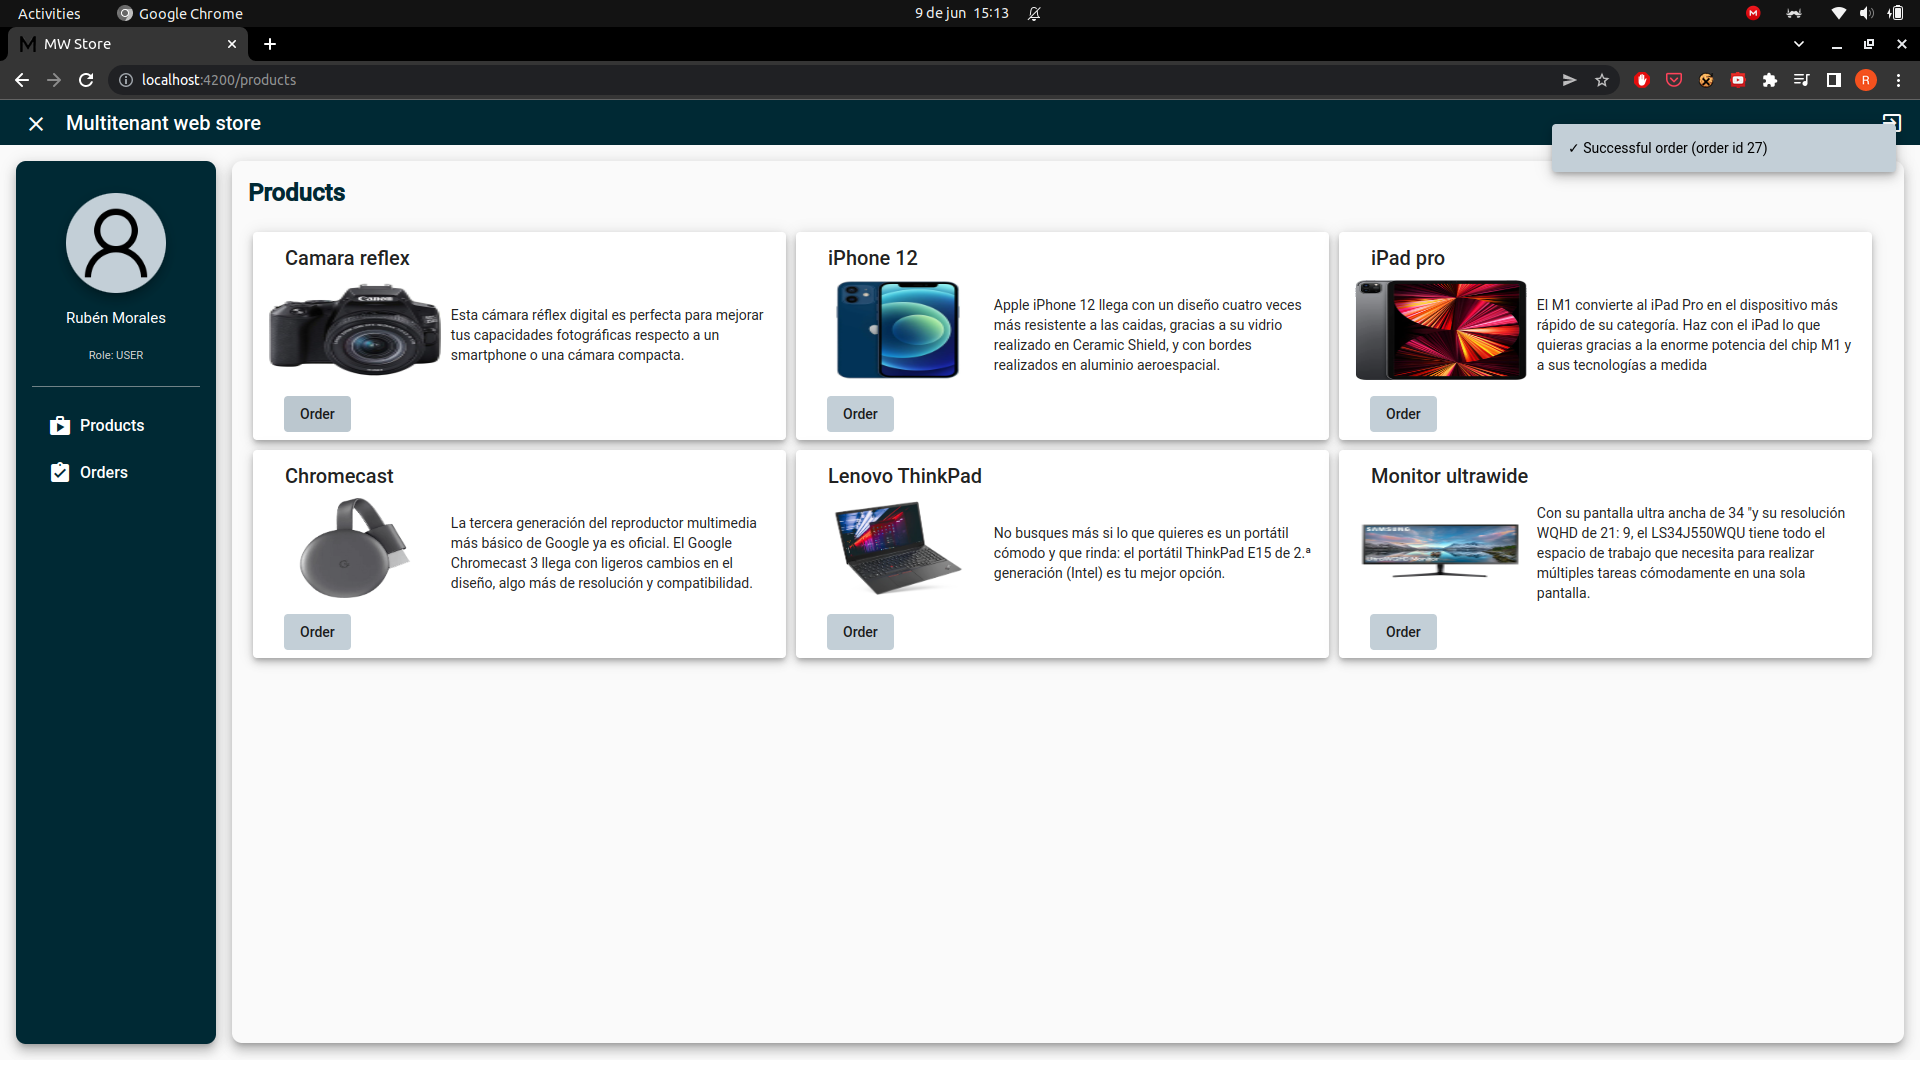
\includegraphics[scale=0.24]{img/mws/ecommerce-multi-tenancy-products.png}
    \caption{Visualization of the products available for one tenant.}
    \label{fig:ecommerce-multi-tenancy-products}
\end{figure}

\begin{figure}[H]
    \centering
    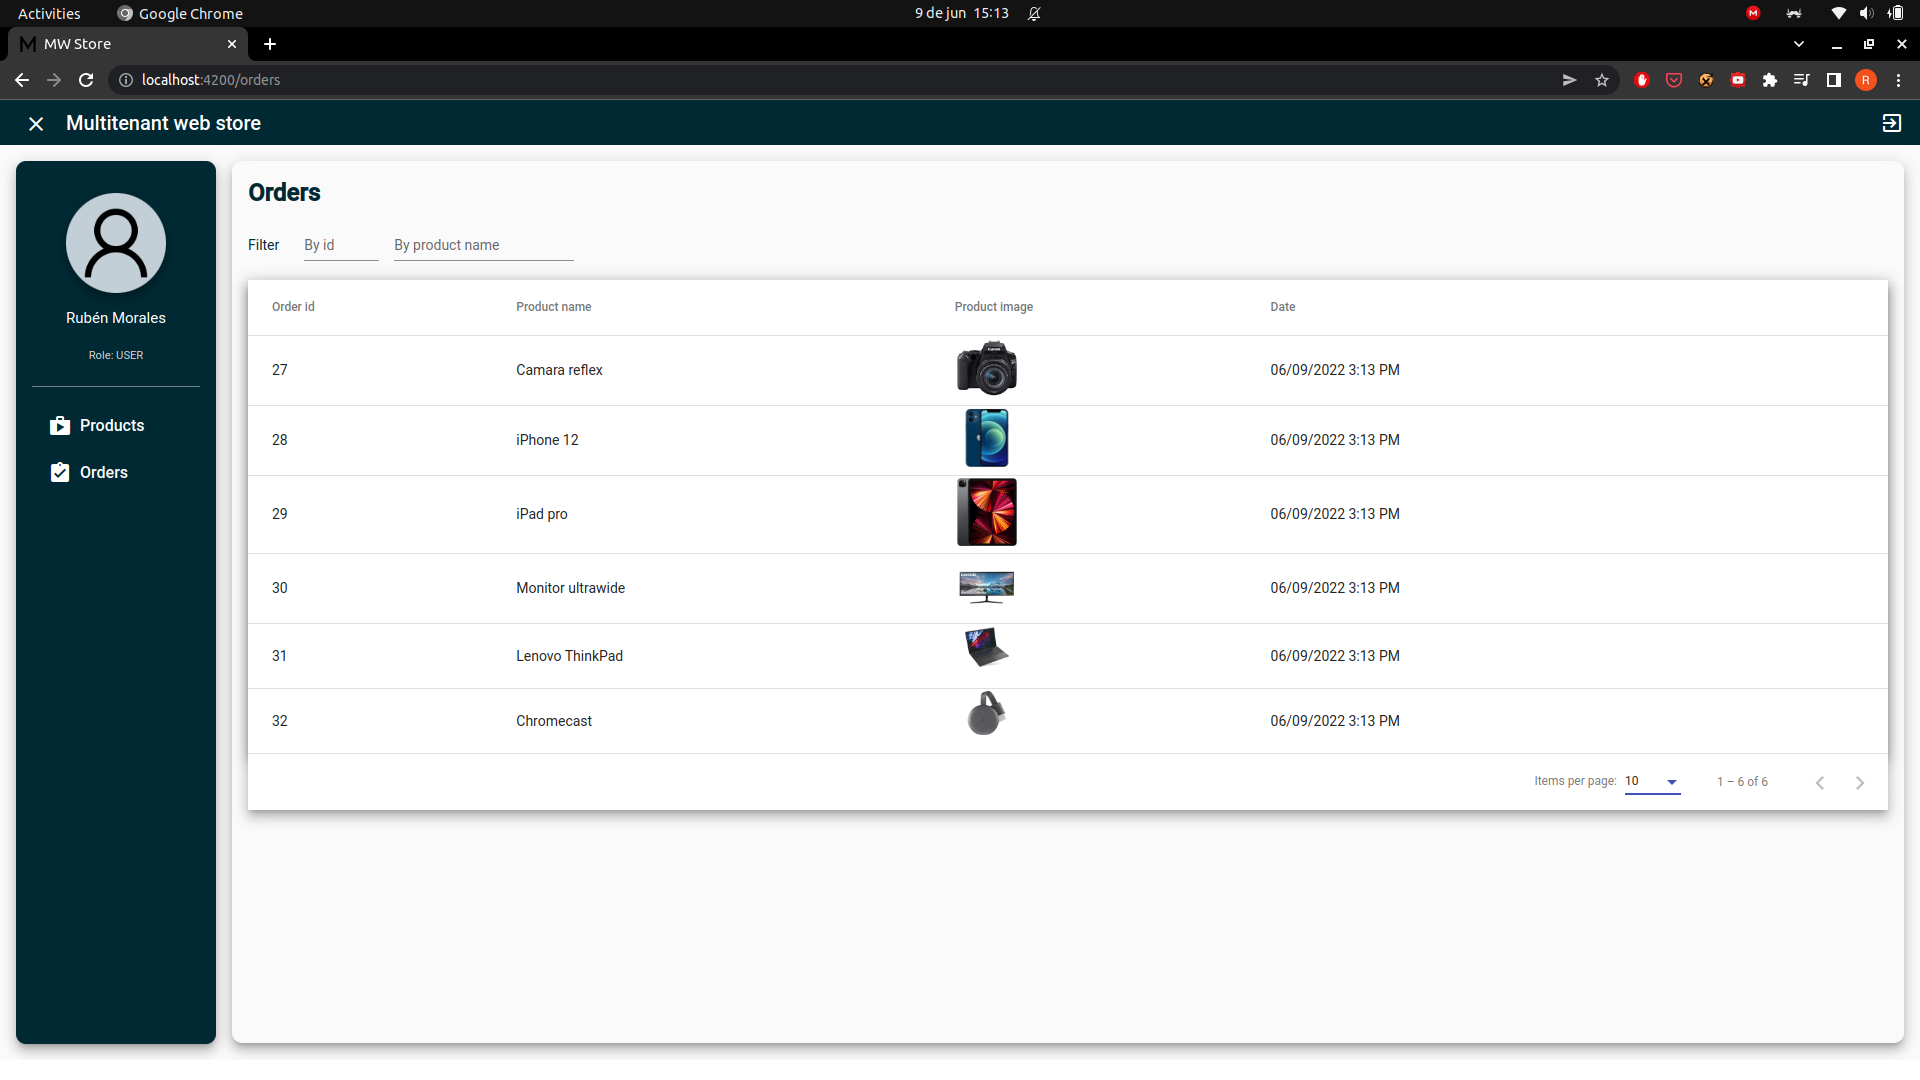
\includegraphics[scale=0.24]{img/mws/ecommerce-multi-tenancy-orders.png}
    \caption{Visualization of the orders available for one tenant.}
    \label{fig:ecommerce-multi-tenancy-orders}
\end{figure}

\

The technological stack of the system is:
\begin{itemize}
    \item Front end: Angular 13.2.7 (testing with Karma + Jasmine)
    \item Back end: Java 17 (testing with JUnit).
    \item Database: agnostic database calls using Hibernate as ORM. (several databases were used as example).
\end{itemize}

The minimal database structure to handle the e-commerce is shown in Figure \ref{fig:ecommerce-database-structure}.
\begin{figure}[H]
    \centering
    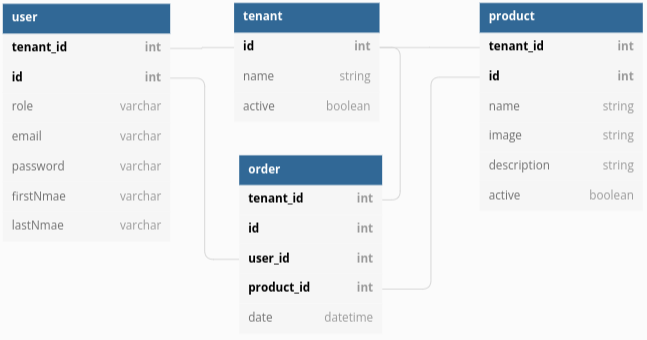
\includegraphics[scale=0.55]{img/mws/ecommerce-database-structure.png}
    \caption{Multi-tenant e-commerce minimal database structure.}
    \label{fig:ecommerce-database-structure}
\end{figure}

\begin{comment}
// Tables in https://dbdiagram.io/d
Table user as U {
  tenant_id int [pk, ref: > T.id]
  id int [pk, increment]
  role varchar [not null]
  email varchar  [not null, unique]
  password varchar [not null]
  firstNmae varchar
  lastNmae varchar
}

Table tenant as T {
  id int [pk, increment]
  name string
  active boolean [default: true]
}


Table product as P {
  tenant_id int [pk, ref: > T.id]
  id int [pk, increment]
  name string
  image string
  description string
  active boolean [default: true]
}

Table order {
  tenant_id int [pk, ref: > T.id]
  id int [pk, increment]
  user_id int  [pk, ref: > U.id]
  product_id int  [pk, ref: > P.id]
  date datetime  [default: `now()`]
}
\end{comment}


\subsection{Colored Petri Net model}
It turns out that the model will be a special kind of producer-consumer (like Figure  \ref{fig:cpn-user-input-choices}, modeling an infinite amount of user choices).
The model heavily depends on the specifications of the system.
Functional specifications determine the properties of the final CPN.
The simplest general multi-tenant e-commerce architecture is used for a better understanding of its properties.
Even with a minimalist model, the resulting Colored Petri Net is not straightforward.
There are several parts of this multi-tenancy e-commerce:
\begin{itemize}
    \item Creation of tenants (businesses).
    \item Creation of final users (buying the products).
    \item Creation of products (by the tenants).
    \item Creation of orders (by the users, with only one product).
\end{itemize}

There are other important properties to model the system:
\begin{itemize}
    \item A tenant must exist to be able to create a user (linked to that tenant).
    \item Only a tenant can create a product.
    \item A product without any associated order and a user must exist to create an order.
\end{itemize}

Let's start with the modeling of tenant creation.

\

\subsubsection{Tenants sub-net}
First, let's create a producer-consumer subnet to represent the tenant creation.
One possible problem of some producer-consumer models with Colored Petri Net is producing an infinite amount of marks.
The possibility of having infinite marks in a place will prevent K-limitation, and it is not a desirable property.
A property to allow the creation of infinite marks is allowing the production of the same mark an indefinite number of times.
The proposed model to solve this is to split the creation of marks between two places: one place with the finite possible values of not created entities and another with the created ones.
These two places are linked using a transition.

\

There are unique constraints when creating a tenant in the database.
The name of the tenant is a possible unique identifier when it is not possible to change it.
To address this issue, the subnet of tenant creation will have three parts (see Figure \ref{fig:mws-cpn-tenant-creation-init}):

\begin{itemize}
    \item Place $P\_NT$: the set of all possible tenants not yet created.
    Each color represents one tenant.
    \item Transition $T\_T$: represents the creation of a new tenant.
    The transition color domain derives from its input transition.
    \item A place, $P\_T$, containing the created tenants.
    \item An arc from $P\_NT$ to $T\_T$, with the set of tenants as input.
    \item An arc from $T\_T$ to  $P\_T$ with the set of tenants as output.
\end{itemize}

\

Another possible way to model the system is using $P\_NT$ as all the possible input values and the transition subset as the valid ones (i.e., tenant names with a maximum length, etc.).
In this model, only one set is used, just for simplicity in the mathematical model.

\

The Figure \ref{fig:mws-cpn-tenant-creation-init} contains a simplified version of the model for tenant creation.
There is only one initial mark in $P\_NT$, representing a possible name for tenant creation using $T\_T$.
The reason to represent the set $TenantSet$ as $\{'e-commerce'\}$ is just simplicity in the view.
Indeed, there would be as many marks as tenant names with less or equal than ten characters.
The tenant sub-net is colored in red to simplify the global picture.

\

\begin{figure}[H]
    \centering
    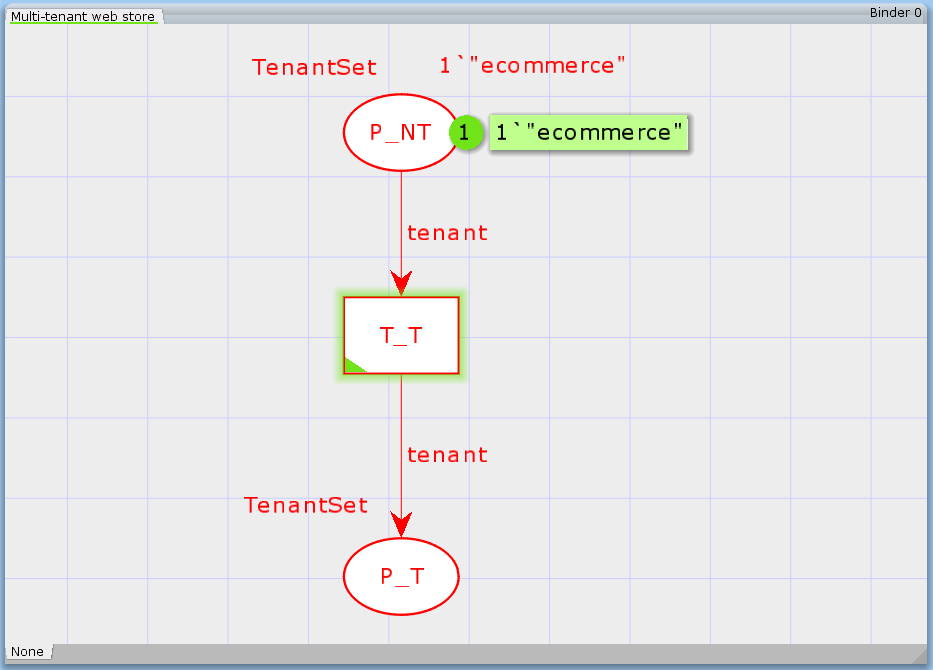
\includegraphics[scale=0.45]{img/mws/cpn/mws_cpn_tenant_init.png}
    \caption{CPN for tenant creation. Initial non created tenant 'e-commerce'.}
    \label{fig:mws-cpn-tenant-creation-init}
\end{figure}                                                                           
                                                                
\
                 
Formally, the sub-net is defined as $TENANT\_SUBNET :=                (P, T, C^-, C^+, \mathcal{C}, cd)$ where
\begin{itemize}
    \item $P = \{P\_NT,\ P\_T\}$
    \item $T = \{T\_T\}$
    \item $\mathcal(C) = \{TenantSet\}$ where $TenantSet := \{a | ...|z \}^{\{1|...|10\}}$
    \item $cd : P\vee T \rightarrow \mathcal{C}$
    where $cd (P\_NT) = cd(P\_T) = cd(T\_T) = TenantSet$
    \item $C^-[p,t] = cd(t) \rightarrow Bag(cd(p))$\newline
    $C^-[p,t] = \begin{cases} 
      \{TenantSet\} & if\  (p=P\_NT\  \wedge\  t=T\_T)\\
      \{\}          & otherwise
   \end{cases}$
    \item $C^+[t,p] = cd(t) \rightarrow Bag(cd(p))$\newline
    $C^+[t,p] = \begin{cases} 
      \{TenantSet\} & if\  (t=T\_T\  \wedge\  p=P\_T) \\
      \{\}          & otherwise
   \end{cases}$
\end{itemize}

\

\begin{figure}[H]
    \centering
    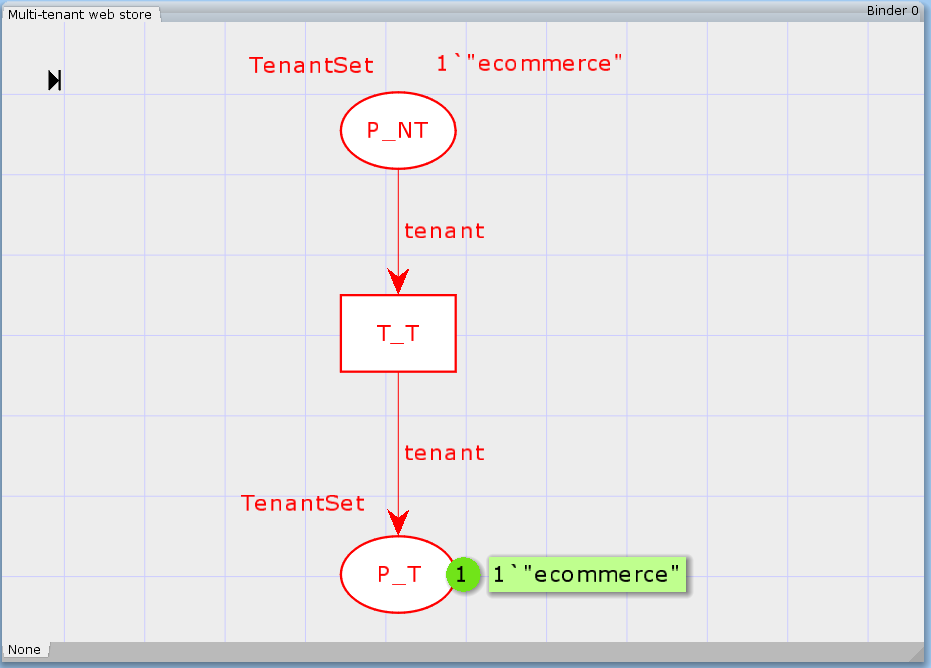
\includegraphics[scale=0.45]{img/mws/cpn/mws_cpn_tenant_created.png}
    \caption{CPN after tenant creation. Now, there is a tenant 'e-commerce' as a mark in $P\_T$}
    \label{fig:mws-cpn-tenant-created}
\end{figure}

The current firing sequence is $\{T\_T\}$.
The next step is to expand this system to allow user creation.

\subsubsection{Users sub-net}
It turns out that a similar (slightly modified) structure should be valid for user creation.
In multi-tenancy, an end user is created just for a specific tenant.
In this scenario, an end-user depends on the desired web store business.
The same person could have several end-users in the system, one (or more) for each web store.
An identical set to $TenantSet$, $UserSet$ stores the possible unique names of the users.

\ 

In Figure \ref{fig:mws-cpn-user-init}, using the same set for $P\_NU$ and $P\_U$ prevents us from having users with the same name in different tenants.
This limitation is artificial and used for simplicity in the model.
Indeed, the correct output set from $T\_U$ would be $TenantSet\times UserSet$ because the tenant information is essential and must be stored.
Due to the limitations of CPNTools, it is impossible to define the Cartesian product of two large sets as an output set: "If a free variable from a large color set is bound to an output arc, an error message will indicate the problem." \cite{cpn-tools-arc-inscriptions}.

\

It is possible to skip this limitation by defining an artificial Cartesian product.
The length limit for tenant names was ten, idem for users.
If $UserSet$ length is extended then we can represent a mark as "user@tenant".
If the arc to create users limits properly the length (allowing only a subset of its input set) the result is equivalent to the Cartesian product.
Anyway, this trick is just useful for educational purposes, showing the user associated with the tenant in the mark.

\

\begin{figure}[H]
    \centering
    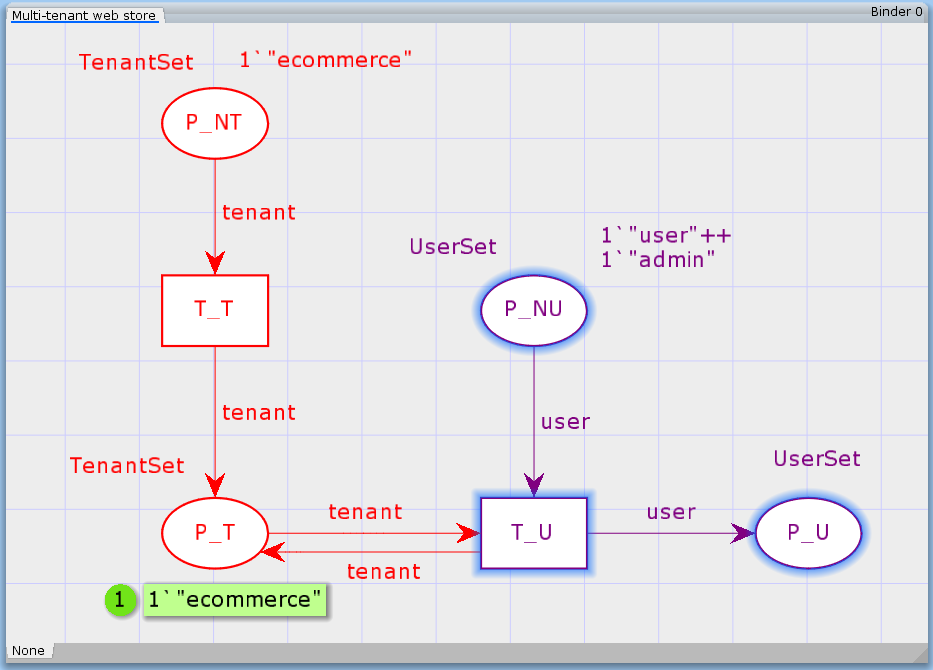
\includegraphics[scale=0.55]{img/mws/cpn/mws_cpn_user_init.png}
    \caption{CPN able to create end users.}
    \label{fig:mws-cpn-user-init}
\end{figure}

\

It is remarkable to notice the two-arc between the $TenantSet$ and the transitions to create users (Figure \ref{fig:mws-cpn-user-init}).
Losing the tenant after the user creation is not a good idea.
The model must represent a system with the possibility of creating several (but a finite number of) users!

\

This approach has a problem, though.
It is incomplete because there are three kinds of users:
\begin{itemize}
    \item Super: the owner(s) of Multi-tenant Web Store.
    They have permission to control the tenants.
    The super user is linked to a special kind of tenant which controls other tenants' metadata.
    There could be several super users, but only a super user can create other super users.
    \item Admin: administrator(s) of each business.
    They have a custom control panel where products are created and orders monitored.
    Only the super user can create new admins.
    \item User: end-user buying the products of one specific web store.
    There is no restriction on the creation of end users rather than unique name constraints.
    Anyone can be a potential user of each e-commerce.
    For that reason, in this model, anyone can create an end user for any business.
\end{itemize}

Three more transitions are needed to differentiate the control flow, one per user type.
The user management subnet is purple.
Let's see how to create the different users, considering the restrictions specified above.

\

\begin{figure}[H]
    \centering
    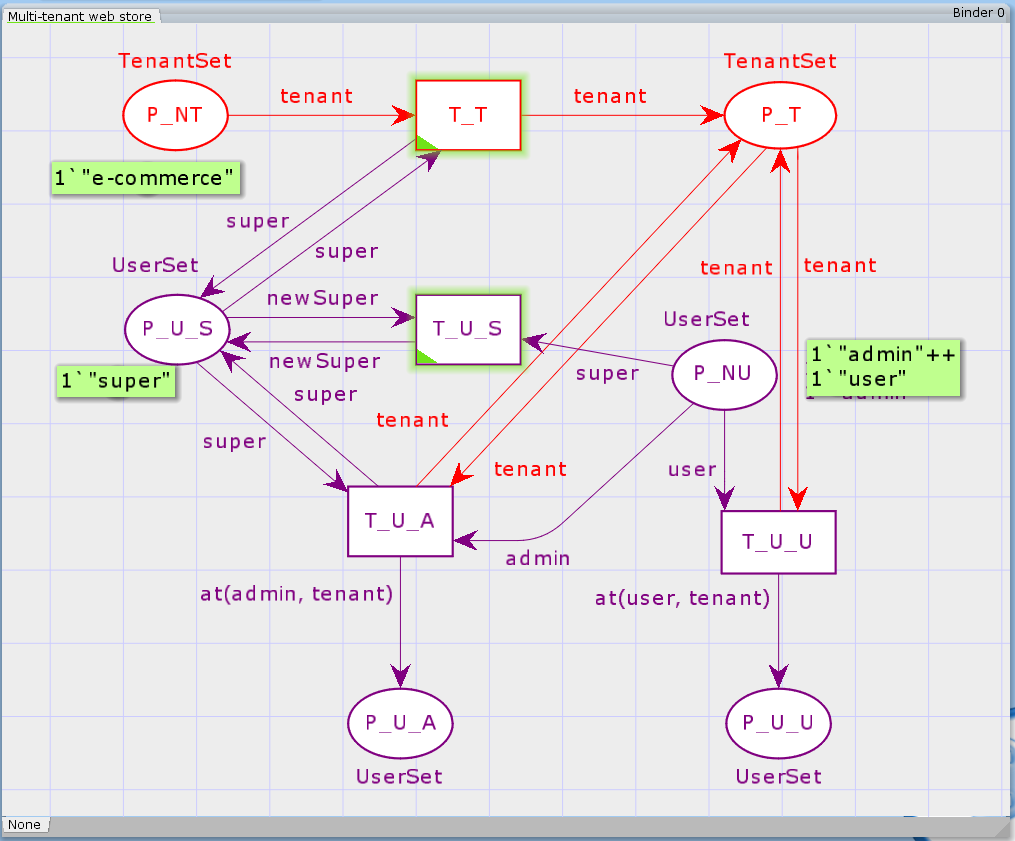
\includegraphics[scale=0.55]{img/mws/cpn/mws_cpn_all_users_initial.png}
    \caption{CPN with all the user's creation logic at the initial marking}
    \label{fig:mws-cpn-all-users-initial}
\end{figure}

\

An important property to consider now is that the system's initial data changed. 
It is not the tenant anymore but the initial super user (see Figure \ref{fig:mws-cpn-all-users-initial}).
The super user is the only initial data in the data store at the beginning.
This super user has the power to create tenants on demand.
There is no magic entity creating tenants but an actual operator (super user) from MWS.
It is debatable if the tenant should also be in the initial system's data.
It is a good practice to minimize the direct manipulation of the database.
Having only the super user as the initial data allow tenant creation with the possible security constraints checked at the application level.
The super user as the only initial data seems like a reasonable idea.
The only user allowed to create super users and tenants is the super user.

\

\begin{figure}[H]
    \centering
    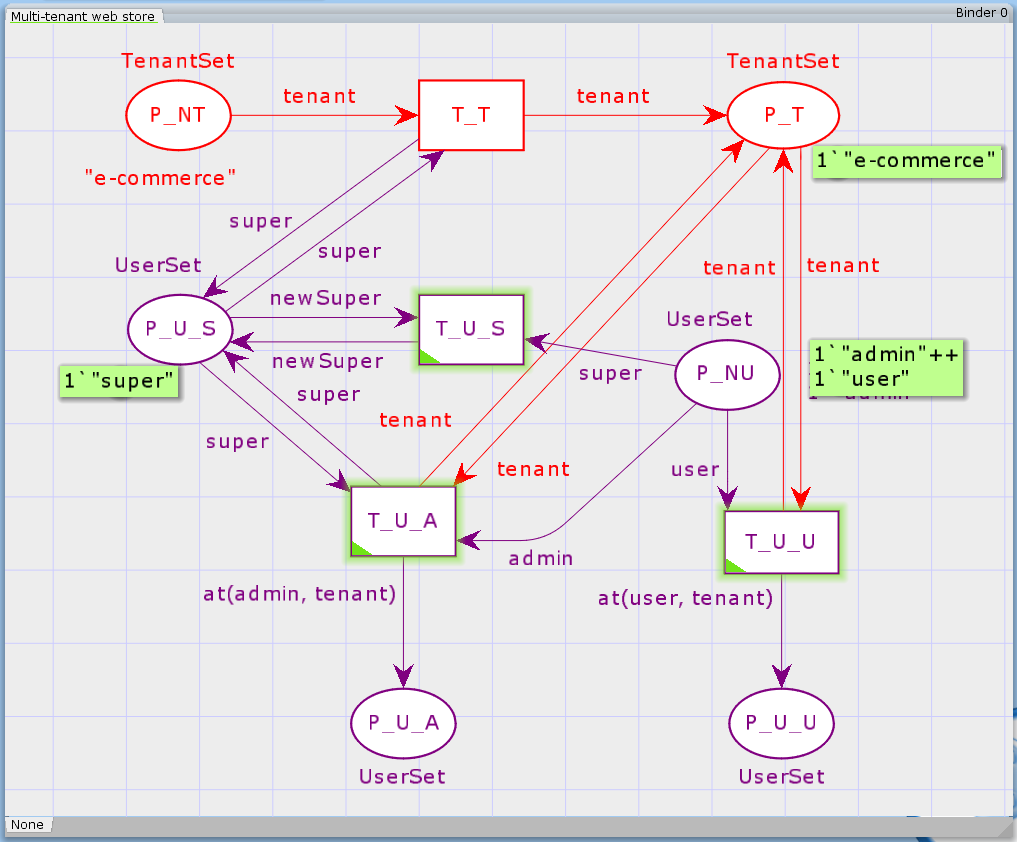
\includegraphics[scale=0.55]{img/mws/cpn/mws_cpn_super_tenant_created.png}
    \caption{CPN with a super user and a tenant created}
    \label{fig:mws-cpn-super-tenant-created}
\end{figure}

\

Now, the way to create tenants has changed to integrate its logic with the user management (see Figure \ref{fig:mws-cpn-super-tenant-created}).
The super user already created a new e-commerce tenant.
After that, the super user can still create more super users because there are no other restrictions for that.
The difference with the previous step is the possibility to create admins.
The admins depend on a tenant to make sense.

\

\begin{figure}[H]
    \centering
    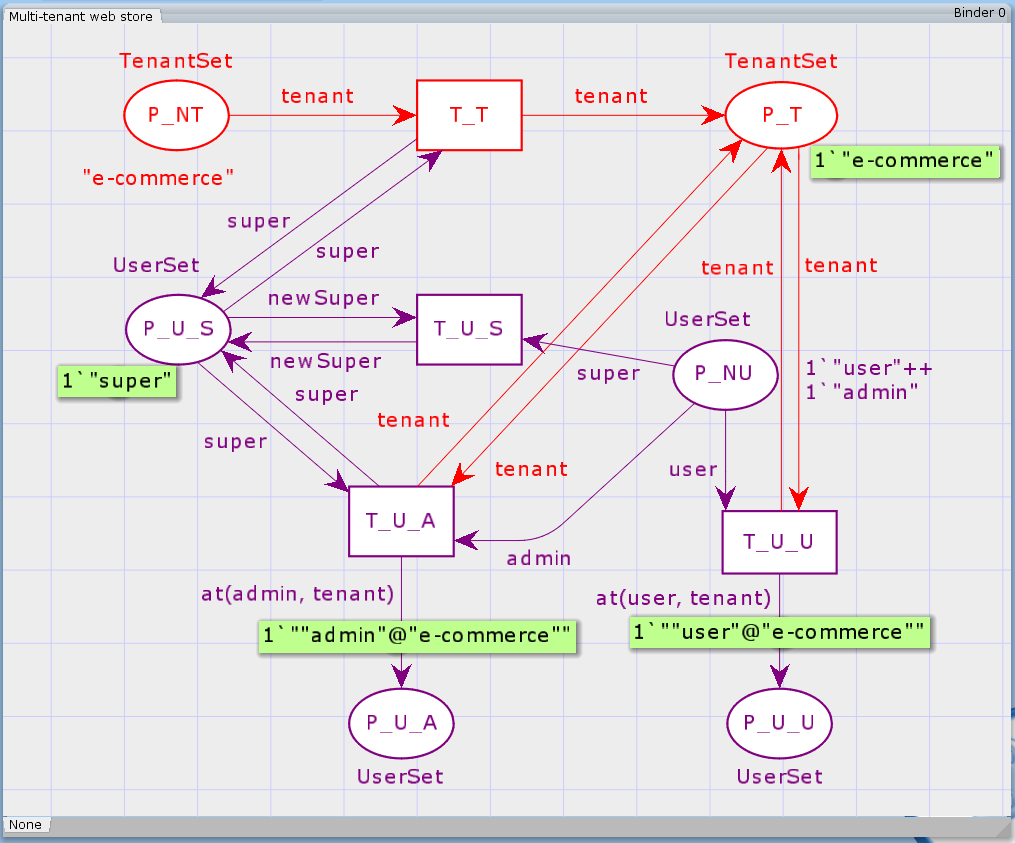
\includegraphics[scale=0.55]{img/mws/cpn/mws_cpn_all_users_created.png}
    \caption{CPN after all users created}
    \label{fig:mws-cpn-all-users-created}
\end{figure}

\

In Figure \ref{fig:mws-cpn-all-users-created} the admin and one user of the e-commerce were created.
There is no enabled transition now because there are no more marks in $P\_NU$ to create super, admins, or end users.
The model will become more complex, so, from now on, we will consider only one tenant, one super user, one admin, and one end user.

\

The previous model(s) changed.
Now, the definition of the net in Figure \ref{fig:mws-cpn-all-users-created} is:

$USERS\_SUBNET := (P, T, C^-, C^+, \mathcal{C}, cd)$,
\begin{itemize}
    \item $P = \{P\_NT,\ P\_T\,\ P\_U\_S,\ P\_U\_A,\ P\_U\_U\}$
    \item $T = \{T\_T,\ T\_U\_S,\ T\_U\_A,\ T\_U\_U \}$
    \item $\mathcal(C) = \{TenantSet, UserSet\}$ where $TenantSet = UserSet = ASCII^{\{1|...|10\}}$ where $ASCII$ is the set of possible characters in the ASCII table.
    The sets $TenantSet$ and $UserSet$, even though they have the same elements, are treated differently to understand the model relationships.
    \item $cd : P\vee T \rightarrow \mathcal{C}$
    where 
    \newline
    $cd (P\_NT) = cd(P\_T) = cd(T\_T) = TenantSet$,
    \newline
    $cd(P\_U\_S) = cd(P\_U\_A) = cd(P\_U\_U) = cd(P\_NU)$
    \newline
    $= cd(T\_U\_S) = cd(T\_U\_A) = cd(T\_U\_U) = UserSet$.
    \item $C^-[p,t] = cd(t) \rightarrow Bag(cd(p))$ \newline
    $C^-[p,t] = \begin{cases} 
      \{TenantSet\} & if\ (p=P\_NT\ \wedge\ t=T\_T)\\
      \{UserSet\} & if\ (t\in\{T\_U\_S,\ T\_U\_A,\ T\_U\_U\})\\
      \{\}          & otherwise
   \end{cases}$
    \item $C^+[t,p] = cd(t) \rightarrow Bag(cd(p))$\newline
    $C^+[t,p] = \begin{cases} 
    \{TenantSet\} & if\  (t=T\_T\ \wedge\ p=P\_T) \\
    \{UserSet\}   & if\  
    
    \begin{cases} 
        t\in\{T\_U\_S,\ T\_U\_A,\ T\_U\_U\} \\
        \wedge \\
        p\in\{P\_T,\ P\_U\_S,\ P\_U\_A,\ P\_U\_U\}
    \end{cases} \\
    \{\}          & otherwise
   \end{cases}$
\end{itemize}

\

The current firing sequence is 
\begin{itemize}
    \item $T\_T$: Creation of a tenant.
    \item $T\_U\_A$: Creation of an admin for the new tenant.
    \item $T\_U\_U$: Creation of the first final user of the system, a client of the created tenant.
\end{itemize}

\

The next step is to integrate the product creation.


\subsubsection{Products sub-net}
The products sub-net follows the same principles of the previous models for producer-consumer.
The proposed subnet (in brown) for product creation is shown in Figure \ref{fig:mws-cpn-basic-product-initial}.

\

\begin{figure}[H]
    \centering
    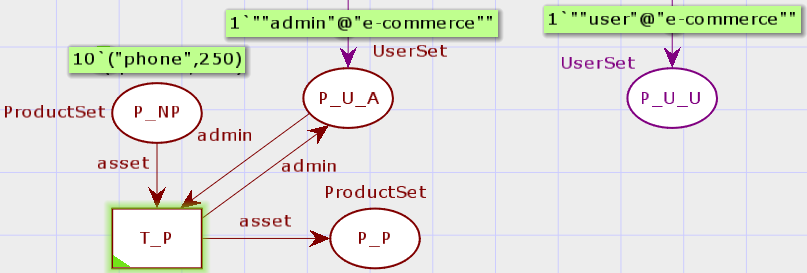
\includegraphics[scale=0.65]{img/mws/cpn/mws_cpn_basic_product_initial.png}
    \caption{CPN for product creation.}
    \label{fig:mws-cpn-basic-product-initial}
\end{figure}

\


The model from Figure \ref{fig:mws-cpn-basic-product-initial} has a relevant limitation.
Even the most basic web store needs the product price and the ability to change it.
The modified net for product management is in Figure \ref{fig:mws-cpn-product-with-price-and-edit}.

\

\begin{figure}[H]
    \centering
    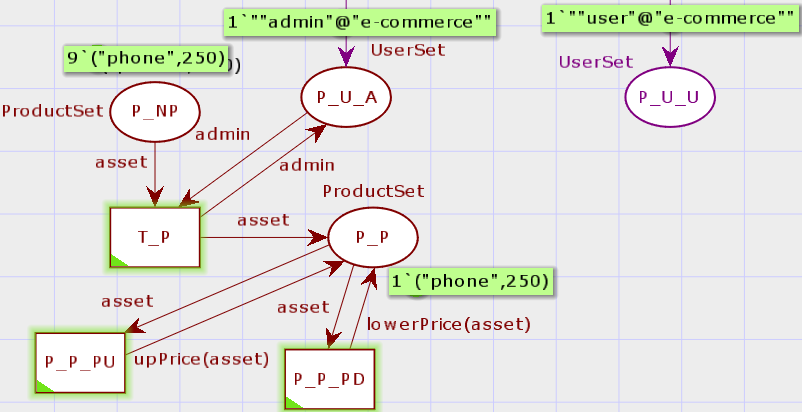
\includegraphics[scale=0.65]{img/mws/cpn/mws_cpn_product_created.png}
    \caption{CPN with product prices creation and update.}
    \label{fig:mws-cpn-product-with-price-and-edit}
\end{figure}

\

In Figure \ref{fig:mws-cpn-product-with-price-and-edit} there are some things that can be improved.
First, the limitation of incrementing or decrementing the product price one by one does not make sense. 
A delta value simplifies the logic, not requiring several transition firings to change the price.
The possible delta values set must be a finite subset of $\mathbb{R}$.
Otherwise, it would not meet the definitions.

\

A user might be involved in a product's price update.
Final users must not change the price.
For security reasons, just the tenant admin of a tenant will be able to manage the product prices (not other tenant products).
This restriction will be verified using an intermediate transition between the place of tenant admins and the place of products.
It is possible (not implemented for simplicity) to make granular permissions to restrict product updates just for a subset of admins.

\

\begin{figure}[H]
    \centering
    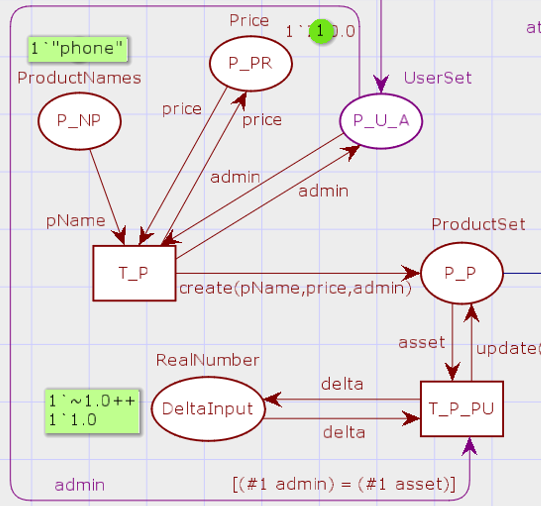
\includegraphics[scale=0.7]{img/mws/cpn/mws_cpn_improved_product_update.png}
    \caption{CPN with improved product management}
    \label{fig:mws-cpn-improved-product-management}
\end{figure}

\

The model will use the improved product management model from Figure \ref{fig:mws-cpn-improved-product-management}.
The product price is updated using a defined method $update(asset, delta)$ that computes the sum of the values.
The idea is to replace a product with its new version in one atomic transaction using transition $T\_P\_PU$.
It is the mission of the last subnet, the modeling of product orders.


\subsubsection{Orders sub-net}
An order in this system is a confirmation of a user action requesting a product.
The assumptions are:

\begin{itemize}
    \item Any available product in their tenant's store can be bought by any user, regardless of its ongoing price.
    \item An order is limited to one product.
    \item There is no limitation on the number of products to order per user.
    \item After order creation, the product will not be available to another end user.
    \item A user can buy any amount of orders.
\end{itemize}

The stock of a product can be simulated shifting the complexity to the data model in $P\_NP$.
There will be no lock to buy a product.
In real life, it is common to prevent product sales to external users when the product is already in other user cart.

\

\begin{figure}[H]
    \centering
    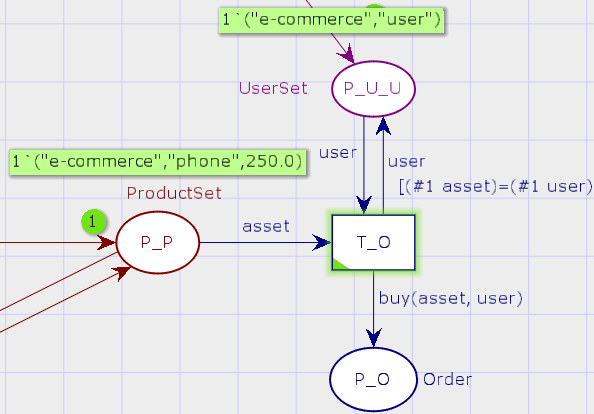
\includegraphics[scale=0.7]{img/mws/cpn/mws_cpn_order_initial.png}
    \caption{CPN to create orders for products.}
    \label{fig:mws-cpn-order-initial}
\end{figure}

\

Figure \ref{fig:mws-cpn-order-initial} show the order management system.
If a user (mark in $P\_U\_U$) and a product (mark at $P\_P$) coexist, then the transition to order products, $P\_O$, is enabled.
Transition $T\_O$ is the last element of the net.
It serves as the order history of all users.

\subsection{MWS Colored Petri Net Analysis}
Finally, Figure \ref{fig:mws-cpn-order-finished} shows the final Colored Petri Net.
It models the Multi-tenant Web Store with an order finished and kept in the order history (place $T\_O$).

\

In summary, now that the whole CPN is defined, here are the minimal transition firings to end ordering a product in MWS.

\begin{itemize}
    \item The initial super user exists, firing $T\_T$ will create a tenant ('e-commerce') indefinitely at $P\_T$.
    \item The $T\_U\_A$ transition depends on the super user and the tenant. Its firing will create an admin for the tenant at $P\_U\_A$.
    \item The independent firing of $T\_U\_U$ creates a user for the tenant at $P\_U\_U$.
    \item The admin in $P\_U\_A$ verifies its existence firing the transition $exists$.
    \item After that, the admin creates a product by firing $T\_P$, storing the new product in $P\_P$.
    \item The product at $P\_P$ and the end user at $P\_U\_U$ enable the transition $P\_O$. $P\_O$ represents the function to buy a product. Its firing will create a purchase record at $T\_0$.
\end{itemize}

\

\begin{figure}[H]
    \centering
    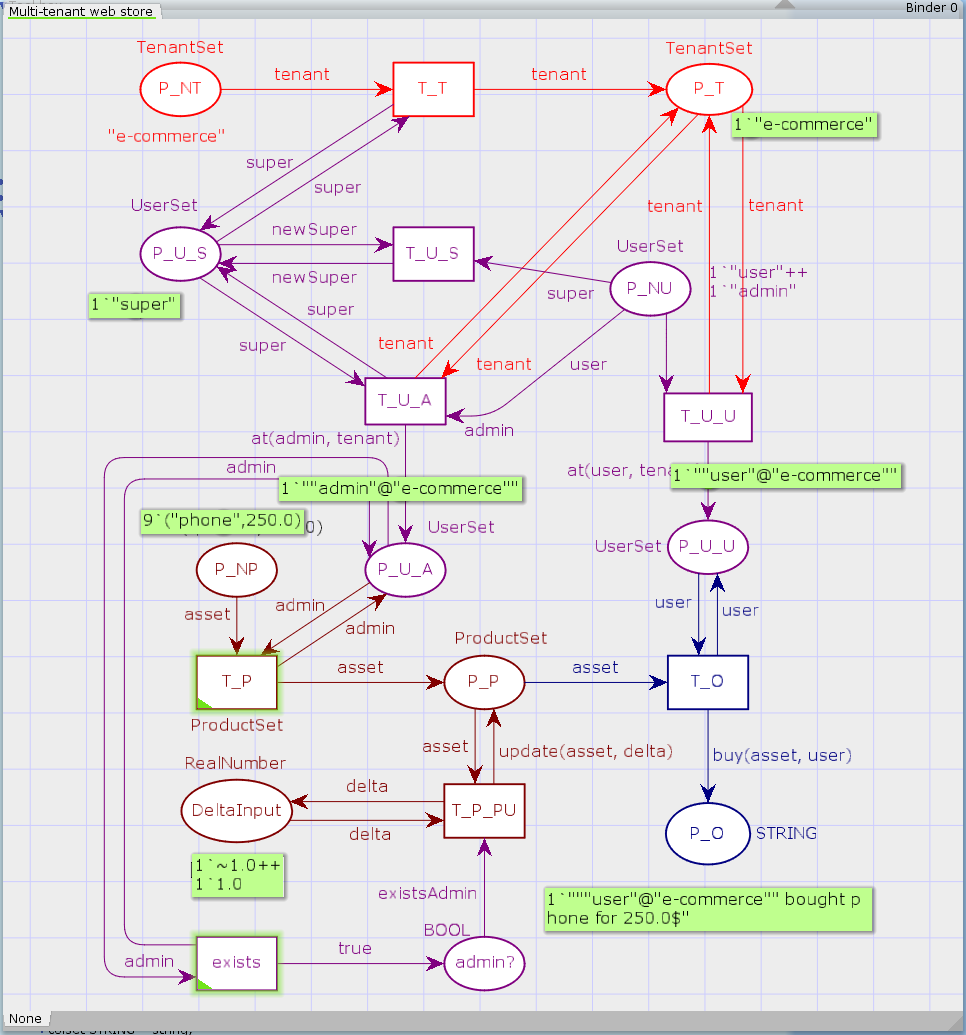
\includegraphics[scale=0.65]{img/mws/cpn/mws_cpn_order_finished.png}
    \caption{Multi-tenant Web Store model with a Colored Petri Net.}
    \label{fig:mws-cpn-order-finished}
\end{figure} % TODO?: show a better image without imprecissions

\

Formally, the definition of the sub-net in Figure \ref{fig:mws-cpn-order-finished} is:

$MWS\_CPN := (P, T, C^-, C^+, \mathcal{C}, cd)$,
\begin{itemize}
    \item $P := \{P\_NT,\ P\_T\,
        \ P\_NU,\ P\_U\_S,\ P\_U\_A,\ P\_U\_U,\ admin?,\ 
        P\_NP,\ DeltaInput,\ P\_P,\  
        P\_O\}$
    \item $T := \{T\_T,\ 
        T\_U\_S,\ T\_U\_A,\ T\_U\_U,\ exists,\ 
        T\_P,\ T\_P\_PU,\ 
        T\_O\}$
    \item $\mathcal{C} := \{TenantSet,\ UserSet,\ ProductSet,\  BOOL,\ STRING,\ RealNumber,\ UserSet\times ProductSet,\\
        STRING\times RealNumber, RealNumber\times ProductSet \times BOOL\}$ where 
    \begin{itemize}
        \item $BOOL := \{true, false\}$
        \item $TenantSet = UserSet = ProductSet = STRING = ASCII^{\{1|...|100\}}$ where $ASCII$ is the set of possible characters in the ASCII table.
        These sets, even though they have the same elements, are treated differently to understand the model relationships.
        \item $RealNumber$ is $\mathbb{R}\cap[-100,100]$ with a maximum number of ten decimals.
        The purpose of this limitation into a finite set is to have the possibility to unfold the net into a simpler General Petri Net.
        It does not include a restriction on the possible uses of updating the price of a product.
        There are no prices with more than ten decimals, and it is always possible to fire the same transition several times if the upper/lower bounds are insufficient.
    \end{itemize}

    \item $cd : P\vee T \rightarrow \mathcal{C}$
    where 
    \begin{itemize}
        \item $cd (P\_NT) = cd(P\_T) = cd(T\_T) = TenantSet$
        \item $cd(P\_U\_S) = cd(P\_U\_A) = cd(P\_U\_U) = cd(P\_NU) = cd(T\_U\_S) = cd(T\_U\_A) = cd(T\_U\_U) = c(exists) = UserSet$
        \item $cd(P\_NP) = cd(T\_P) = cd(P\_P) = ProductSet$
        \item $cd(admin?) = BOOL$
        \item $cd(T\_O) = STRING$
        \item $cd(DeltaInput) = RealNumber$
        \item $cd(P\_O) = UserSet\times ProductSet$
        \item $cd(P\_NP) = STRING\times RealNumber$
        \item $P\_P\_PU = RealNumber\times ProductSet \times BOOL$
    \end{itemize}
    \item 
    $C^-: P\times T \rightarrow Bag(cd(P))$ is a matrix of functions:\newline
    \begin{blockarray}{ccccccccc}
        T\_T & T\_U\_S & T\_U\_A & T\_U\_U & exists & T\_P & T\_P\_PU & T\_O \\
        \begin{block}{(cccccccc)c}
        IDTS &0          &0          &0          &0          &0          &0          &0          & P\_NT \\
        0  & 0 & IDTS & IDTS &0          &0          &0          &0          & P\_T \\
        0 & IDUS & IDUS & IDUS & 0 & 0 & 0& 0 & P\_NU \\
        IDUS & IDUS &IDUS          &0          &0          &0          &0          &0          & P\_U\_S \\
        0 & 0 & 0 & 0 & IDUS & IDUS & 0 & 0 & P\_U\_A \\
        0 & 0 & 0 & 0 & 0 & 0 & 0 & IDUS & P\_U\_U \\
        0 & 0 & 0 & 0 & 0 & 0 & IDB & 0 & admin? \\
        0 & 0 & 0 & 0 & 0 & IDSR & 0 & 0 & P\_NP \\
        0 & 0 & 0 & 0 & 0 & 0 & IDR & 0 & DeltaInput \\
        0 & 0 & 0 & 0 & 0 & 0 & IDPS & IDPS & P\_P \\
        0 & 0 & 0 & 0 & 0 & 0 & 0 & 0 & P\_O \\
        \end{block}
    \end{blockarray}

    \item $C^+: T\times P \rightarrow Bag(cd(P))$:\newline
    \begin{blockarray}{ccccccccc}
        T\_T & T\_U\_S & T\_U\_A & T\_U\_U & exists & T\_P & T\_P\_PU & T\_O \\
        \begin{block}{(cccccccc)c}
        0 & 0 & 0 & 0 & 0 & 0 & 0 & 0 & P\_NT \\
        0 & 0 & IDTS & IDTS & 0 & 0 & 0 & 0 & P\_T \\
        0 & 0 & 0 & 0 & 0 & 0 & 0 & 0 & P\_NU \\
        IDUS & IDUS & IDUS & 0 & 0 & 0 & 0 & 0 & P\_U\_S \\
        0 & 0 & ATAT & 0 & 0 & IDUS & 0 & 0 & P\_U\_A \\
        0 & 0 & 0 & 0 & 0 & 0 & 0 & IDUS & P\_U\_U \\
        0 & 0 & 0 & 0 & exists & 0 & 0 & 0 & admin? \\
        0 & 0 & 0 & 0 & 0 & 0 & 0 & 0 & P\_NP \\
        0 & 0 & 0 & 0 & 0 & 0 & IDR & 0 & DeltaInput \\
        0 & 0 & 0 & 0 & 0 & IDPS & 0 & 0 & P\_P \\
        0 & 0 & 0 & 0 & 0 & 0 & 0 & buy & P\_O \\
        \end{block}
    \end{blockarray}
\end{itemize}


Having: 
$$IDTS: TenantSet\rightarrow 1\hspace{0.5cm}IDTS(x)=1 \hspace{0.5cm}\forall x\in TenantSet,$$
$$IDUS: UserSet\rightarrow 1\hspace{0.5cm}IDUS(x)=1 \hspace{0.5cm}\forall x\in UserSet,$$
$$IDSR: STRING\times RealNumber\rightarrow 1\hspace{0.5cm}IDSR(x)=1 \hspace{0.5cm}\forall x\in  STRING\times RealNumber,$$
$$IDR: RealNumber\rightarrow 1\hspace{0.5cm}IDR(x)=1 \hspace{0.5cm}\forall x\in RealNumber,$$
$$IDB: B\rightarrow 1\hspace{0.5cm}IDB(x)=1 \hspace{0.5cm}\forall x\in B,$$
$$IDPS: ProductSet\rightarrow 1\hspace{0.5cm}IDPS(x)=1 \hspace{0.5cm}\forall x\in ProductSet,$$

$$ATAT: UserSet\times TenantSet\rightarrow UserSet\hspace{0.5cm}ATAT(u,t)=concat(u,"@",t) \hspace{0.5cm}\forall (u,t)\in UserSet\times TenantSet,$$
$$buy: UserSet\times ProductSet\rightarrow UserSet\hspace{0.5cm}buy(u,p)=concat(u, " bought ", p) \hspace{0.5cm}\forall (u,p)\in UserSet\times ProductSet,$$
$$exists: UserSet\rightarrow 1\hspace{0.5cm}exists(x)=1 \hspace{0.5cm}\forall x\in UserSet,$$


It is clear that when the number of places or transitions increases, the matrices become huge.
Even though they are mostly zero matrices, the operation cost of real-world problems becomes complex.

\

The initial marking in $MWS\_CPN$ is

$$
\begin{aligned}
  M_0 := & (\{'e-commerce'\},\{\}, \ \{'admin', 'user'\},\ \{'super'\},\ \{\}, \\
         &\  \{\}, \ \{\}, \{('phone', 250.0')\},\ \{1.0, -1.0\},\ \{\},\ \{\})
\end{aligned}
$$


There are some relevant problems with this model, though.
Supposedly, each tenant should be independent of the others.
The product does not store information about the tenant.
Any end user can buy all the tenant products!
It is mandatory to keep track of the tenant associated with the data.
Hereinafter, all the data related to a tenant will use the Cartesian product for its definition.
The definition of all tenant related elements will have the structure 
$$(tenantName, identifier)\hspace{0.8cm} tenanName\in TenantSet,\ \ identifier\in\mathcal{C},$$
for proper visibility checks.
An example of this Cartesian product is shown in Figure \ref{fig:mws-cpn-secure-net}, see place $P\_U\_S$ where the super user mark is a composition of its tenant and user name.
The tenant linked to the super user is a meta-tenant allowed to handle the information of all the tenants.

\

Transitions can have restrictions based on the value of their input values.
This possibility is equivalent to having a restriction on the input subset.
In Figure \ref{fig:mws-cpn-secure-net} these issues are fixed:
\begin{itemize}
    \item Transition $T\_O$ is not be enabled for products and users from different tenants.
    \item Only admins can create and modify products.
\end{itemize}


\

\begin{figure}[H]
    \centering
    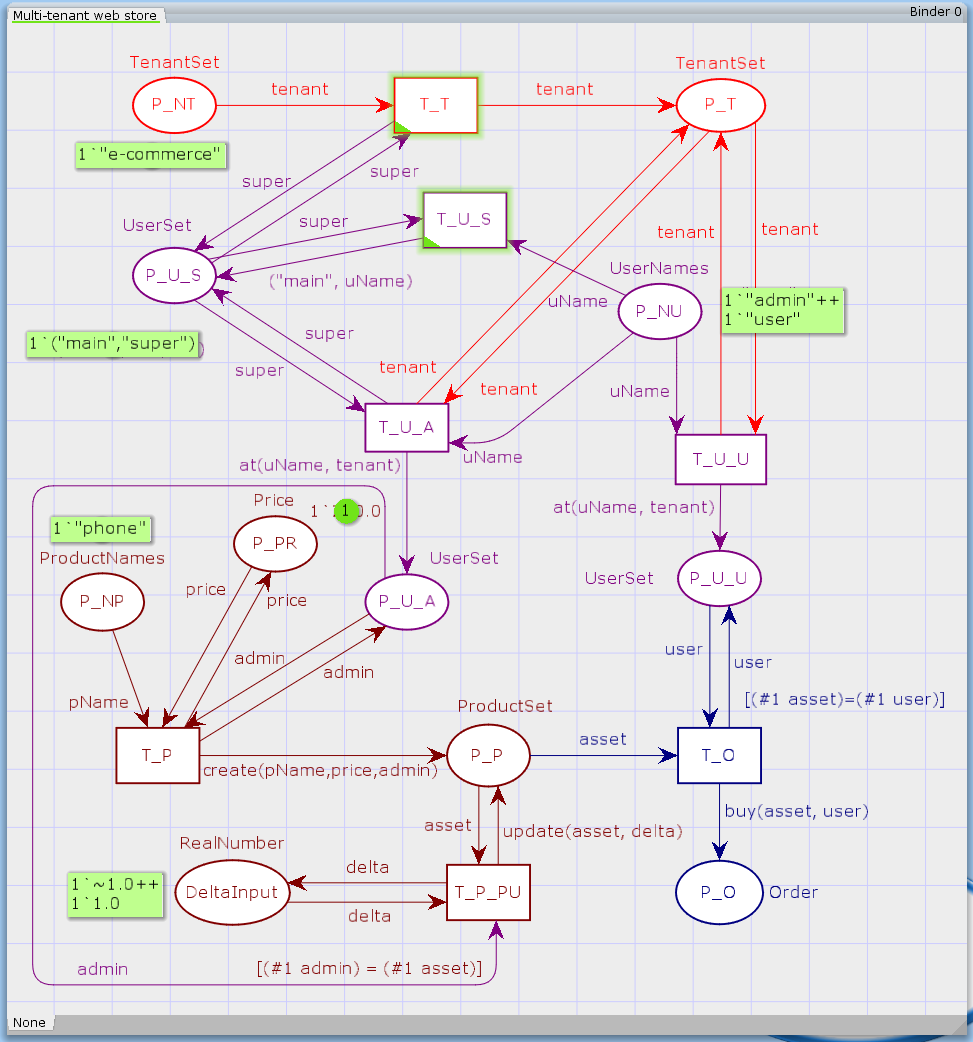
\includegraphics[scale=0.65]{img/mws/cpn/mws_cpn_secure_net.png}
    \caption{Multi-tenant Web Store secure model with a Colored Petri Net}
    \label{fig:mws-cpn-secure-net}
\end{figure}

\

The CPN in Figure \ref{fig:mws-cpn-secure-net} have several properties that will be discussed.

First, let's discuss security.
The Net is K-limited with $K:= \sup\{|cd(p)| : p\in P\} > 1$, verifying that the supremum is actually a maximum. 
Therefore, the net is not secure since it is not 1-limited.

\

Security is a very tough property not present in many nets modeling real-world systems considered safe.
There is a trade-off between security and liveness.
The decisions made in the design of the CPN prioritize more secure nets at the cost of liveness.
The color domains are finite to represent the system database limitations at a given moment.
If the system needs more resources, a color domain redefinition is required.
It can be argued that the model should not be modified but represent all the theoretical resource needs.
In that scenario, the net would improve its liveness properties at the cost of reduced K-limitation.
The reachability net of the MWS CPN is finite.

\

% Figure \ref{fig:mpn-security-property-summary} implies that the net is not strictly conservative, not conservative, not structurally limited.

To study if the net is conservative, we need to check if there is any transition generating infinite values or losing values.
Most system transitions move marks from some places to others, without modifying the total number of marks.
It is relevant to remember the distinction between conservative and strictly conservative net regarding the number of marks.

\begin{itemize}
    \item $T\_T$: the super user does not change, and the tenant mark moves to $P\_T$.
    \item $T\_U\_S$: one mark moves from $P\_NU$ to $P\_U\_S$.
    \item $T\_U\_A$: one mark moves from $P\_NU$ to $P\_U\_A$.
    \item $T\_P$: moves one product name mark to create a product.
    \item $T\_P\_PU$ does not generate any mark. It just changes the product price.
    \item $T\_U\_U$: moves one mark from the user names to create a mark in users.
    \item $T\_O$: moves one mark from the products to the orders.
\end{itemize}

It turns out that the number of marks is kept constant.
The net is not just conservative, also strictly conservative and (see Figure \ref{fig:mpn-security-property-summary}).
The net is not repetitive.
It is possible to detect cycles in some subnets, but definitely not in the whole net.
There is a clear path for the flow of data.

\

The data is created on demand, but the amount of tenants/users/products/orders is finite.
If all the tenants create all the possible products, users, and orders, then there will be no possible transition to be fired.
The trade-off here is K-limitation. We could sacrifice K-limitation to have infinite sets and have alive transitions.
Therefore, the net is not alive, nor structurally alive.
% {\color{red}Habría que rediseñar la red para que fuera viva o parcialemnte viva; una red "muerta" como la que se discute, no tendría gran utilidad; ten en cuenta que el modelo del productor-consumidor, en el que parece que basas tu modelo, no tiene por qué dar lugar a una red que se bloquea cuando se agotan los recursos}
It acts as a complex producer-consumer model with limited resources.
This limitation can be bypassed if necessary with color domain extensions.

\

About conflicts, transitions $T\_U\_S,\ T\_U\_A,\ T\_U\_U$ are in an effective conflict.
They all depend on a finite set of inputs to be enabled.
The moment with just one mark in $P\_NU$ will have a conflict to choose the type of the last user to create.
The concurrent nature of multi-tenancy approaches makes this kind of model inherently conflictive.
In practice, since the tenants' data is logically separated at the application level, the conflicts are fewer than might appear at first glance.

\

The model does not show the specific database used.
The restrictions of the same tenant for any product, user and order creation/modification represent the system's functional requirements.
It is crucial to have tenants' data, at least, logically separated without direct access and/or modification from other tenants.
The CPN model is database agnostic.
It is independent of the usage of different databases, schemas or shared schemas.
It just needs the data flow requirements.
The order creation depends on the user (which is a functional requirement for purchases) and the product chosen.
This information is convenient because it shows that the model is elastic until the product level.
Elasticity at the product level means that, with vast sudden traffic demands, sharding data is allowed until product granularity in different databases.
Therefore, it is possible to use dynamic scaling algorithms to split products into several databases on demand.
The multi-tenant nature of the system makes dynamic scaling easier because it can be applied to all the tenants at the same time.

\

% {\color{red}Habría que redefinir el modelo para cumpliera las propiedades de ser estructuralmente limitada y viva, ya que si demostramos eso, entonces se puede demostrar la garantía de ser una red repetitiva y conservativa, para la que no habría ningún problema en calcularle el arbol de alcanzabilidad!}
It is not feasible to handle the version of the reachability graph for this CPN (the occurrence graph) for all the scenarios.
The complexity of generating the occurrence graph by hand is prohibitive.
Only a computer can generate and analyze it with a certain guarantee of no errors.
CPN Tools does not include tools to generate this graph
Anyway, the relevant point is to understand the data flow in the model.

\begin{itemize}
    \item First, any super user creates one or more tenants
    \item New users are created for the tenant (admins and end users)
    \item The admins of the tenant create/edit the products \textbf{only for its tenant}.
    \item The end users buy the products available in its tenant.
\end{itemize}

It turns out that there is only one possible data flow and a finite number of firings.



\newpage


\section{Quality of Service in Cloud Environments}
In multi-tenant models, each tenant uses a fraction of the resources.
Indeed, resource usage is very efficient when the tenant's load is not highly correlated.
This tenant interdependency might hinder the quality of service defined in the Service-level agreement (SLA) with the client.

\

It is critical from the business perspective to ensure availability, performance, and elasticity of multi-tenant Cloud applications like MW-Store.
The mean load might be relatively more stable when including more tenants.
The problem is that the potential variance in traffic might affect response times if the system cannot scale adequately.
Deficiencies in this model will affect all tenants simultaneously, breaking several SLAs.
Any human intervention is slow and inefficient compared to a well-designed automated system.
The principal scalability objective is to ensure dynamic adaptation to uneven loads without human intervention, verified with spike testing.

\

Enterprise software could potentially be used simultaneously by a lot of people.
Performance is relevant in multi-tenant applications where a bottleneck affecting one customer could potentially affect several customers.
We need to distinguish between data scaling (increased capability to store and handle data) and application scaling (total workload that the application can handle) \cite{multi-tenant-data-architecture}.

\

Databases can scale up to increase server resources (memory, processors, disk speed, etc.) or scale out (a database partition into several servers) \cite{multi-tenant-data-architecture}.
It is desirable to model the data clusters to optimize the read and write operations in a database.
Dynamic scaling involves automatic detection and processing of resource usage metrics.
Examples of metrics include CPU, memory, disk usage, etc.
Based on the thresholds defined for these metrics, automatic triggers will perform scaling actions.
It is also convenient to optimize resource usage by automatic descaling when needed.


\subsection{Metrics}

The minimum Quality of Service (QoS) without penalties is defined in a contract with each tenant called a Service-level agreement (SLA) \cite{cooper2009}.
% TODO: cite (Cooper et al., 2009).
Although the performance of the algorithms is relevant, database calls involving network incurs into a big percentage of the request latency.
Adaptation to sudden load increases is critical to guarantee the restrictions of the SLAs
\cite{elmore2011}. 
% Todo: cite s (Elmore et al. 2011).

\

By extension, response times must be under control in databases.
This task is particularly difficult since the database handles all the concurrent data access abnormalities.
QoS might involve response time limits.
Dynamic bottleneck discover using spike tests helps to reduce maximum response times.

\

If not handled correctly, the system failures is the sum of all its components failures.
Hardware failures are improbable, but possible.
Its relevance could be reduced paying higher prices for Cloud services specialized in fault tolerance.
Network failures are possible.
Do not rely on network.
There are different strategies to minimize the effect of network issues, e.g. network calls retry, idempotency, data replication, smart servers, Exactly-Once stream-processing (frameworks like Kafka allow this configuration by default), etc. 

\

Some system properties must be verified to ensure QoS compliance:


\begin{itemize}
    \item Elasticity: adaptation of the available resources to the necessary ones to handle the current system load without the stop-the-world problem.
    \item Availability: understood as the percentage of time when the system is reachable with valid responses.
    The interval of time without service between failures is reduced using self-healing and replication factor greater than one in container orchestration systems like Kubernetes.
    The application code scalability is simpler than data scalability due to the absence of state.
    When a program grows, it is desirable to split the code into different packages, creating independently deployable modules.
    A well-known availability measure is 9’s. 3 nines uptime means that a system is fully operational 99.9\% of the time \cite{availability-nines-measure}.
    \item Load balance: it is desirable to have an evenly distributed load in the different system instances (application(s) and database(s)). Automatic load balancing provides maximum throughput with minimal response times \cite{shimonski2003}. 
    % TODO: cite (Shimonski, 2003)
    Good load balancing might help achieve better elasticity (allowing more reaction time to adapt the system) and availability (reducing the risk of lack of resources. E.g. out of memory errors).
\end{itemize}

\

Another problem is the inter-dependency between tenants.
A sudden load in a tenant could potentially affect all the tenants if the system is not elastic enough.
In the real world, the data of one tenant is not usually directly accessible from another.
The database must minimize tenant interference.
It sounds straightforward, but the data store model must consider specific approaches to prevent this kind of interdependency.
Techniques like data split, indexes, defined foreign keys, and so on minimize the data access interdependency.



\subsection{Data scalability}
Scalability must be taken into account in all parts of the system, including data stores.
Otherwise, even if the application is extremely fast there will be a data access bottleneck.
Application containers are stateless, making scalability a lot easier because it is possible to use load balance and automatic scaling approaches (i.e. using Kubernetes).
With a certain amount of information or users, having the data only in one database is simply not feasible.
If the application has only one data store, its resources are limited and also depend on a single-point-of-failure.

\

There are two approaches to achieving data scalability.

\begin{itemize}
    \item Horizontal scalability (or scale-out): it includes new running instances to increase the number of possible handled requests.
    It is the most general and relevant technique.
    The downside of this approach in data stores is that it forces data migrations between data stores in critical scenarios.
    \item Vertical scalability (or scale-up): increase resources in a running instance, like a server.
    There are two possible implementations: partial redimension and total replacement.
\end{itemize}


There are two general horizontal data scalability patterns, replication, and partitioning.


\subsubsection{Replication}

Replication consists of creating different copies of a database (or database subset), ensuring their data integrity by synchronizing the replicas with the main database \cite{multi-tenant-data-architecture}.
When write operations are only allowed to the original database, it is called single-master replication.
When it is possible to write into several copies of the database is called multi-master replication and requires a more complex synchronization mechanism to integrate the changes between the different copies.
It is a proper approach to select subsets of data in the database that are not modified frequently, and use single-master replication.
Replication has the advantage of being potentially useful as a synchronized data backup.
If the master database is down, it is possible to use the replica, preventing application outages.
This increased security will only be successful if there is independent hardware in the master database and the replica database (i.e. different servers).
Uncorrelated failures are extremely important.
Otherwise, there would not be any security improvement.


\

There are several synchronization techniques.
The synchronization techniques can be divided into two groups:
\begin{itemize}
    \item Synchronous: Imagine that there is a change in the master data store.
    Then, before completing the update, the value in the other replicas will be invalidated/updated.
    There is no fraction of time when the data in the replicas is outdated.
    These techniques favour consistency at the cost of speed while updating.
    This kind of approach is desirable in scenarios where consistency must be kept at all costs, improving performance in other parts of the application.
    \item Asynchronous: Imagine the same change in the master data store.
    Then, the change will be applied to the master data store, even if that means there will be a fraction of time when data is outdated in the replicas.
    It favours speed over consistency, having eventual consistency because at some point the data in the replicas will be updated.
\end{itemize}

\

The data synchronization process is not trivial and still has several trade-offs for scalability and resilience.
The ACID transactions become more complicated with distributed data. In some cases, a database transaction depends on the transaction(s) of another data store(s).
A safe policy in a distributed transaction commit is to roll back by default. Only stop the rollback if a successful response is received. 
This approach enforces transitions resilient to partition tolerance and network issues.
There are several protocols for distributed consensus in distributed data stores, like 2PC, 3PC or MVCC \cite{distributed-consensus-data-replication}. 

\begin{itemize}
    \item 2 Phase Commit (2PC) \cite{distributed-transactions-2pc}: in the first phase, a coordinator asks the different databases to create transactions in a prepared state, flushed into the disk.
    The database does not consider these rows on reads.
    If the whole transaction is later verified as finished, then update the row to a done state.
    The problem is that there are several data stores.
    It is theoretically possible to commit to one database and then have a network error with another.
    If the outage is solved, the data store that was down reviews the commit in a prepared state.
    \item 3 Phase Commit (3PC) \cite{distributed-transactions-3pc}: evolution of 2PC. It attempts to solve the blocking problem if the coordinator is down.
    There is a new intermediate phase called pre-commit.
    The first phase is the same, ask the distributed databases to flush a transaction in a prepared state.
    If a predetermined number of data stores, $k$, respond to the initial request, a second message is sent to pre-commit the transaction.
    At this point, if the coordinator is down, a new coordinator is assigned.
    Thanks to the restriction of $k$ responses, the new coordinator can continue the transaction if at least one of the data stores has the pre-commit state.
    \item Multi version concurrency control (MVCC) \cite{distributed-consensus-data-replication}: multiple versions of the same data are stored.
    PostgreSQL uses it to handle transactions.
    It is possible to choose dynamically between consistency or latency.
    In scenarios where eventually consistency is reasonable, this property removes locks between reads and writes.
    When strict consistency is required, the protocol returns the last version of each element with a possible cost of speed. 
\end{itemize}

Now we will see the other data scalability pattern.

\


\subsubsection{Partitioning}


In partitioning, subsets of the database are moved to other locations/databases.
\begin{itemize}
    \item In horizontal partitioning, a database table is divided into several databases maintaining its structure and reducing the number of rows handled by each database.
    This is also called sharding and require a mechanism to join the resources together, and ensure correctness of the queries.
    Load balancing redirects traffic to the required sharded database(s).
    In order to distribute the rows of the database in several ones a distribution algorithm is needed.
    That algorithm must optimize the even distribution of data, like the module operator.
    The problem with the module operator is that it is not optimal to dynamically add or remove databases for dynamic horizontal scaling, since the ratio of data to move would be too high.
    Other techniques like consistent hashing with virtual nodes decrease data redistribution when adding/removing database servers on demand.
    % TODO?: advanced dynamic database scaling used in DynamoDB: https://twitter.com/alexxubyte/status/1559204532545921024
    \item In vertical partitioning, the columns of a table are split into several tables that will have the same number of rows that the original table.
    This technique is useful when a monolithic application is split into several modules.
    Splitting the tables in a schema into several subsets allows for independently modules deploy.
    As a rule of thumb, database divisions should minimize the number of cross-database communications, keeping related tables in the same database.
\end{itemize}

It is possible to create horizontal partitioning in a shared database based on tenant ids.
Different tenants can have very different demands.
It is necessary to prevent overtaxed partitions while other partitions are underused, i.e. partition the database to balance the number of requests on each database.

\

Using partitioning also reduces the single-point-of-failure issue.
If data is properly distributed (related data kept together) then one part of the distributed data store can be down but most of the requests can still succeed using the other data stores.
Partitioning can be used combined with replication for increased security and availability, at the cost of complexity and potential eventual consistency.



\ 

\subsection{Database types}
It is relevant to study how different databases behave under load.
The concurrent nature of multi-tenant applications makes this study especially important.
Different databases have distinct goals, use cases and trade-offs.
There are two main approaches to fetch data:
\begin{itemize}
    \item SQL (Structured Query Language): this query language to interact with data is typically linked to relational databases.
    These relational databases store data in tables and allow checking the foreign table relationships at the database level.
    MySQL or PostgreSQL are examples of relational databases.
    \item NoSQL (Not-Only relational or Non-relational): it does not define the relationships, allowing extra flexibility but delegates the checks of the possible hidden relationships in the data.
    There is no standard query language for NoSQL.
    Each NoSQL database defines its query language, adapted to the topology of the database.
    UnQL (Unstructured Query Language) is a super set of SQL attempt to standardize a query language for NoSQL databases.
    UnQL allows querying data in JSON or document formats.
    % TODO?: expand about UnQL?
    % UnQL: A Query Language and Algebra for Semistructured Data Based on Structural Recursion
    % https://www.researchgate.net/publication/2458246_UnQL_A_Query_Language_and_Algebra_for_Semistructured_Data_Based_on_Structural_Recursion
    Redis or MongoDB are examples of non relational databases.
\end{itemize}

The relational model is arguably more structured but it has some scalability problems with high volumes of data \cite{type-of-nosql-databases}.
NoSQL database systems relegate consistency management to create a more scalable data storage.
Inside NoSQL databases there are several types \cite{type-of-nosql-databases}:
\begin{itemize}
    \item Key-Value Store Databases: the key and the value are string.
    Typically, the key is a simple type, and the value can represent a serializable object of a programming language.
    Examples are Redis or Amazon DynamoDB.
    \item Column-Oriented Databases: each item has a key related to one or more column(s).
    The NoSQL database more similar to SQL ones, but the internal storage method is distributed and optimizes column operations.
    An example of this type of database is Cassandra.
    \item Document Store Databases: data is stored as documents using a key.
    Documents are flexible records without a fixed schema, allowing formats like XML, PDF or JSON.
    These databases are more complex than key-data ones but allow more granular searches filtering by document fields, reducing network latency.
    Examples are MongoDB or CouchDB.
    \item Graph Databases: data is stored as objects (nodes) and their relationships (edges).
    These edges are pointers to the adjacent nodes.
    It is considered semi-structured data, there are relationships between the nodes, and each node is schema-less.
    Rollbacks are supported as well as the ACID properties.
    An example of a native graph database is Neo4j.
    \item Object Oriented Databases: data is stored as objects and offers object-oriented features like data encapsulation, polymorphism and inheritance.
    Objects can are referenced with pointers for faster access.
\end{itemize}

Not all the databases are directly comparable.
Redis, for example, is an in-memory cache and compared SQL databases are not (although they might use some kind of in-memory cache to improve performance).
The performance differences are shown in Figures \ref{fig:query-performance-databases}, \ref{fig:query-performance-sql-nosql} and \ref{fig:query-performance-oracle-mogodb}.
It turns out that there are relevant differences between SQL and NoSQL databases that deserve some comments.

\

\begin{figure}[H]
    \centering
    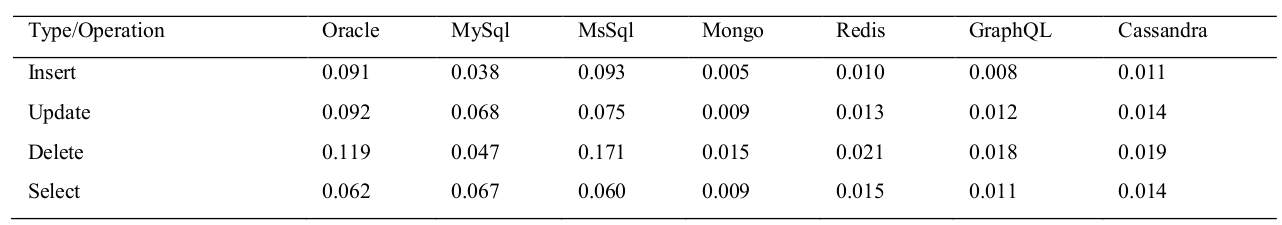
\includegraphics[scale=0.37]{img/db/performance/query-performance-databases.png}
    \caption{Query performance of database with 100 000 records in milliseconds \cite{comparison-query-performance-relational-and-non-relational-databases}.}
    \label{fig:query-performance-databases}
\end{figure}

\

The numbers show a clear advantage of NoSQL vs SQL databases.
They are different databases, created for different purposes.
Redis is an in-memory cache, but it is surprising the magnitudes of MongoDB vs relational databases.
The results of the CREATE/UPDATE/READ/DELETE are combined for approximate overall comparisons in Figures \ref{fig:query-performance-sql-nosql} and \ref{fig:query-performance-oracle-mogodb}.

\

\begin{figure}[H]
    \centering
    \includegraphics[width=0.625\linewidth]{img/db/performance/query-performance-sql-nosql.png}
    \caption{Query performance in milliseconds \cite{comparison-query-performance-relational-and-non-relational-databases}.
    \label{fig:query-performance-sql-nosql}}
\end{figure}

\

\begin{figure}[H]
    \centering
    \includegraphics[width=0.625\linewidth]{img/db/performance/query-performance-oracle-mogodb.png}
    \caption{Query performance for Oracle (green) and MongoDB (blue) \cite{comparison-query-performance-relational-and-non-relational-databases}.
    \label{fig:query-performance-oracle-mogodb}}
\end{figure}


\

NoSQL databases store data in compact entities, allowing fast manipulation.
SQL databases encourage normalization, reducing redundancies and undesirable consistency issues by dividing tables into smaller ones connected through relationships.
These relationships enforce a structure in the data model but prevent the database to reach the performance of NoSQL.

\

The performance tests must include all the intermediate steps of a process.
Figure \ref{fig:network-worldwide-ping-tests} compares the magnitude of ping response times worldwide.
It turns out that for relatively small amounts of data, the performance differences are not a big deal \cite{comparison-query-performance-relational-and-non-relational-databases}.
The problem might arise with extensive amounts of data and complex data relationships enlarging the performance difference due to internal data representation differences between SQL and NoSQL databases.

\

\begin{figure}[H]
    \centering
    \includegraphics[scale=0.65]{img/cloud/network-worldwide-ping-tests.png}
    \caption{Response times for google.com in ten different locations. Tool: https://tools.keycdn.com/ping).}
    \label{fig:network-worldwide-ping-tests}
\end{figure}


\

At this point, there is a trade-off between performance (or potential scalability) and flexibility against structure, reduced duplicity and consistency guarantees.
It can be argued that flexibility is not a massive advantage.
In the multi-tenancy customization section, several extensibility patterns of the data model were proposed.
It was pointed out that some databases, like PostgreSQL allow JSON column types with custom queries.

\

Consistency trade-offs will be discussed in the next section, comparing the different database transaction models.
Then, performance will be compared, for multi-tenancy scenarios, in the section of 'Quality of Service in Cloud Computing'.


\subsection{Comparison of Database Transaction Models}
There are some relevant differences between the different databases types, like transaction models.
A transaction is a set of instruction(s) considered a single unit, handling system's state.
In SQL databases, a transaction begins, then it succeeds (the transaction is committed and persisted to the database) or fails (some databases support rollbacks command to prevent any change in the database if a transaction fails).
Sometimes a transaction is divided into several transaction units.
If any of these unit fails, the whole transaction is marked as a failure.
Most relational database systems guarantee the ACID properties \cite{acid-base-database-transaction-processing}: Atomicity, Consistency, Isolation and Durability.

\begin{itemize}
    \item Atomicity: All the tasks inside a transaction are applied, or none.
    One task failing implies that the whole transaction fails and nothing is committed.
    This property prevents partial writes into the database.
    \item Consistency: The transactions always verify the constraints of the system.
    They can not be committed leaving an inconsistent state in the database.
    \item Isolation: Every transaction is independent and has no access to the information of other unfinished transactions.
    \item Durability: After transaction persistence, it is not possible to revert its effects, and they will be resilient to breakdowns in the system.
\end{itemize}

\

These ACID properties are a safety net at the database level, allowing to have reliable data storage.
After a certain amount of load, the need for data store scaling created new challenges and encouraged the review of the ACID restrictions.
A relational database can still be horizontally scalable using distributed databases.
But, due to its table structure, the performance of the queries depends on the number of tables involved.
Handling data in a tree structure(s) allows the database to store the data physically closer and makes distributed databases easier to scale by design.

\

It is possible to fetch data using the root of the three as id.
This possibility to fetch all the data together allows for improved performance.
A potential problem in distributed databases is queries that force a full scan of all the databases.
If the application continuously scans all the databases filtering for a field, then the advantages of this distribution are under threat.

\

Storing data in a tree structure(s) is more flexible than table structure(s).
As we saw previously, data customizability patterns can be defined in relational models, even though some of them could act as a black box.
Some relational databases (like PostgreSQL) allow having column(s) with JSON format (with the possibility to query inside the JSON fields), having the advantages of the relational model and the flexibility of the tree structure.

\

On the other hand, NoSQL databases focus on performance, scalability, and flexibility.
The origin of the popularity of the term BASE is thanks to Dr Eric Brewer in the Symposium "Towards Robust Distributed Systems" \cite{acid-base-database-transaction-processing}
NoSQL does not support transactions \cite{comparison-query-performance-relational-and-non-relational-databases} and will not always guarantee ACID properties, having softer constraints: Basically Available, Soft state and Eventual consistency (BASE) \cite{acid-base-database-transaction-processing}.

\begin{itemize}
    \item Basically Available: There is a certain degree of availability even with some node unavailability.
    The trade-off here is to allow data to be outdated for the benefit of increased availability.
    \item Soft state: Data consistency is not always guaranteed.
    The returned data could not be the latest state.
    \item Eventual consistency: There is a mechanism to update the data in all the data storage.
    It is guaranteed to have a consistent state eventually.
\end{itemize}

The BASE paradigm can be used as relaxed constraints when approximate answers are tolerable.
ACID paradigm is more suitable for conservative scenarios where data must guarantee to be consistently updated, sacrificing availability.
When the availability is sacrificed, then it is possible to send multiple requests, but returned data is guaranteed to be fresh.
If consistency is not a must, it is possible to create mechanisms to minimize this issue.
For example, in data updates, before updating the master data, mark the data in the nodes as outdated.
ACID is better suited for applications that are constantly inserting and updating data and want this layer of security.
BASE is better for applications that needs extreme performance in read-only operations.

\

Another possibility is to combine both systems.
It is possible to have the core system verifying ACID for insert(s)/update(s) and data replications with BASE properties to have better scalability.
It turns out that the ACID vs BASE debate is a spectrum that depends on the specific system requirements.
This trade-off is described for any distributed data storage.

\subsection{Distributed data store trade-offs}
When an application needs to access data, there is a layer between that application and the data store.
This layer could be a network call between two servers or a process inside the same server.
Hereafter, it will be referred to as a distributed data store because it can be generalized to any data allocation between one or multiple servers.
What happens if the link with the data store breaks?
Are there any potential issues while writing and reading data concurrently?
The formalism to properly define these concepts will be shown.
Then, a discussion about their limitations and possible trade-offs depending on the system requirements.

\

It turns out that in distributed data stores it is not possible to have complete availability and data consistency simultaneously.
That limitation is formally stated in the CAP theorem.
The original article proving the CAP theorem named it the ''Brewer's Conjecture and the Feasibility of Consistent, Available, Partition-Tolerant Web Services'' \cite{brewer-conjecture-cap}.
It references a limitation of distributed web services viewed as asynchronous network models.

\

\theorem{Brewer's Conjecture (CAP)}{It is impossible for a web service to provide the following three guarantees:
\begin{itemize}
    \item Consistency
    \item Availability
    \item Partition-tolerance
\end{itemize}}

\

The Brewer's Conjecture presented lacks concise definitions and proof.
The formal demonstration requires several definitions not included in this project but can be found in \cite{brewer-conjecture-cap}.
It is considered one of the precedents in the debate about the limitations in the design of ACID databases.
The traditional view of interaction with the database behaves as a transaction.
An operation is atomic when it is completed (committed) or fails without intermediate states.
Consistency is the impossibility of inconsistent data at any time that does not verify the rules defined in the database.
Isolation means that a transaction does not have information about other transactions.
It is possible to detect overlapping writes that could lead to inconsistent data and verify transaction isolation since the transaction could have information about the previous system state.
The previous system state does not necessarily mean having information about other transactions.
Several transactions can finish before our operation without having information about them.
The only knowledge is that there was a data change.
Another property is durability, understood as the impossibility of rolling back a change when complete.
Sensitive critical information should still have this strong consistency because it is the final security layer of a critical system.

\



% TODO
% Maurice P. Herlihy and Jeannette M. Wing. Linearizability: A correctness condition for concurrent objects. ACM Transactions on Programming Languages and Systems, 12(3):463-492, July 1990
% Leslie Lamport. On interprocess communication - parts I and II. Distributed Computing, 1(2):77-101, April 1986.


Consistency is a very general term.
There are more specific definitions of consistency, with different properties, granularity, etc.
Some of these consistency types are \cite{acid-base-database-transaction-processing}:

\begin{itemize}
    \item Strict Consistency: Every read provides the last updated value.
    If there are data replicas, all must return the same value after any write operation in one of them.
    \item Eventual Consistency: reads could return outdated value.
    The only guarantee is that, at some point, all replicas will return the same value.
    \item Monotonic Read Consistency: reads could return outdated value.
    It guarantees that if there are several reads over the same object, the client will receive either a previous value or a more updated value.
    \item Read Your Own Writes: when there is an update (independently of the replica to write), the client always receives that updated value, no matter the requested replica node.
    \item Causal Consistency: causally related writes must be seen by all processes in their written order. % TODO?: example here
    \item Linearizability: % TODO?: talk about sequential consistency or serializability
    It is a way to describe concurrent operations as a sequence of non-blocking instantaneous events verifying the First In First Out (FIFO) property.
    A system is linearizable when all its objects are.
    A formal definition with writes and reads operations is described in \cite{linearizability-correctness-condition-for-concurrent-objets}.
    The intuitive consequences are that after an instant modification of a resource, any posterior read operation will see that value if there is no other modification (see Figures \ref{fig:linearizable-operations} and \ref{fig:no-linearizable-operations}).
\end{itemize}

\begin{figure}[H]
    \centering
    \includegraphics[width=0.65\linewidth]{img/db/operation/linearizable-operations.png}
    \caption{Linearizable operations \cite{linearizability-question-stackoverflow}. Read operations always return the latest write.
    \label{fig:linearizable-operations}}
\end{figure}

\begin{figure}[H]
    \centering
    \includegraphics[width=0.7\linewidth]{img/db/operation/no-linearizable-operations.png}
    \caption{No linearizable operations in a data store with a replica  \cite{linearizability-question-stackoverflow}. A node reads a value in the replica before the previous write operation sync and then tries to write in the primary data store.
    The system is not linearizable since the data replication is asynchronous.\label{fig:no-linearizable-operations}}
\end{figure}


There are other examples of consistency guarantees, i.e. FIFO, sequential, entry, casual+, consistent prefix, release, or bounded staleness.
It is clear now that the different consistency definitions might impact the other two properties (Availability and Partition Tolerance) of the CAP theorem.
That is the motivation for the \textit{PACELC theorem} to increase the granularity of the consistency definition.

\

The \textit{PACELC theorem} suggests that, in a distributed system, with a partition (P), it is only possible to choose between (A) or (C) (Availability or Consistency), else (E), without partitions, there is still a trade-off between (L) and (C) (Latency or Consistency) \cite{trade-offs-fault-tolerant-distributed-computing-databases}.

\

It applies softer constraints to the scenario of just one partition, allowing the possibility to change availability with just latency.
The possible combinations of distributed replicated systems: PC/EC, PC/EL, PA/EL, and PA/EC.
% TODO?: expand PACELC theorem
% https://www.cs.umd.edu/~abadi/papers/abadi-pacelc.pdf
Other authors consider that the relationship between availability and consistency should be a continuum, from weak to strong, with eventual consistency in the middle \cite{trade-offs-fault-tolerant-distributed-computing-databases}.




\begin{comment}

{\color{red}
\subsection{Modelo de BD Multi-inquilino
}
La selección de un modelo de multi-inquilinato se ve actualmente como una
tarea primordial cuando se construye una base de datos para proporcionar servicios de SGBD (IaaS) desde el Cloud.

El número, la naturaleza y las necesidades de los inquilinos que se espera
atender también afectan a la decisión de la arquitectura de datos en diferentes formas. 
%
Algunas de las siguientes preguntas pueden llevarnos a decidir un enfoque
más aislado, mientras que otras pueden inclinarnos a adoptar un enfoque más colaborativo.

¿Cuántos posibles inquilinos esperamos tener? Quizá no podamos estimar el
número de manera objetiva, pero si podemos pensar en términos de magnitud:

¿Estamos desarrollando la aplicación para cientos? ¿Para miles? ¿Decenas de miles? ¿Más? Cuanto mayor sea el número estimado, más debemos considerar una opción compartida.

¿Cuánto espacio de almacenamiento espera que necesitará de media cadainquilino? Si pensamos que alguno o todos los inquilinos almacenarán una gran cantidad de datos, quizá sea mejor utilizar un enfoque más aislado como un modelo de base de datos separada. 

De hecho, grandes requerimientos de espacio pueden forzarnos a adoptar dicho modelo de base de datos separada de todos modos. 
%
Por esto será mucho más fácil diseñar la aplicación de esa manera desde el principio.

¿Cuántos usuarios concurrentes esperamos que soporte de promedio el
inquilino? El número de conexiones se puede ver comprometido en el enfoque
compartido, por tanto, un aislamiento de datos mejorará las prestaciones al cliente.

¿Ofrecemos servicios adicionales de copias de seguridad y restauración? En
este caso, dichos servicios son más fáciles de ofrecer a través de un enfoque más aislado.

Se suele adoptar el modelo \emph{multi-inquilino de base de datos compartida}, es decir, con esquemas separados (o instancias compartidas), por ser el más utilizado y presentar la mejor relación entre utilización de recursos, rendimiento y seguridad (Barker et al. 2012).

Según el modelo anterior, cada máquina virtual tiene una instancia del SGBD, y cada SGBD contiene una cantidad variable de inquilinos, dependiendo de la capacidad de los recursos de la máquina virtual y la carga de trabajo. Un inquilino se representa mediante una base de datos en el sistema. 
%
A pesar de exigir menos recursos de infraestructura, este modelo aumenta la interferencia entre los inquilinos, ya que existe mayor concurrencia de inquilinos en el mismo SGBD.

La interferencia entre inquilinos se produce cuando el aumento de la carga de trabajo de un inquilino altera el rendimiento de otros inquilinos que están siendo ejecutados en el mismo SGBD. 
%
La elección del SGBD ayuda a reducir las interferencias, así como es
necesario analizar el perfil del inquilino para determinar el nivel de interacción con otros inquilinos y seleccionar la mejor asignación para evitar las interferencias.
%
Una buena estrategia es aislar inquilinos susceptibles de interferir entre ellos.

Para analizar la interferencia en un entorno de SGBD Multi-inquilino
seguimos la metodología elaborada en (Moreira et al., 2012), que consiste en un conjunto de experimentos para verificar la disponibilidad y la interferencia en un SGBD multi-inquilino en la Nube. 

Los siguientes pasos se suelen definir para lograr una correcta ejecución de los experimentos:

\begin{enumerate}
    \item Definir el modelo multi-inquilino que vaya a ser utilizado.
    \item Definir los benchmarks necesarios para generar el ambiente de SGBD multi-inquilino.
    \item Definir los SGBDs y el alojamiento de los inquilinos en estos sistemas.
    \item Definir las cargas de trabajo, a lo largo del tiempo, para cada inquilino.
    \item Analizar la variación de carga de trabajo y su relación con la
disponibilidad de cada inquilino.
\end{enumerate}

}



\subsection{Quality of Service Model for DDBB in Cloud Computing}
% TODO: compare database performance (MySQL, PostgreSQL, MongoDB, MariaDB, ...)
{\color{red}

Nuestro modelo de SGBD en el Cloud con calidad de servicio se construirá
atendiendo a los requisitos de elasticidad, escalabilidad y uso eficiente de los recursos. 

Como ayuda a la definición del modelo, identificamos un conjunto de
metas y desafíos:

\begin{enumerate}
    \item Es necesario cumplir el acuerdo de nivel de servicio (SLA)
    \item  Agregar fácilmente inquilinos al sistema sin interrumpir el servicio del resto de inquilinos existentes
    \item Calcular los recursos computacionales necesarios para el funcionamiento de cada nuevo inquilino y, al mismo tiempo, atender a las restricciones de todos los inquilinos que comparten la misma instancia del SGBD
    \item Identificar factores limitantes o cuellos de botella en los recursos computacionales requeridos por las diferentes instancias, cada una con varios inquilinos, que contienen diferentes restricciones que deben ser atendidas.
    \item Durante la distribución de los inquilinos es necesario indicar la mejor ubicación para evitar que se produzcan violaciones del SLA
    \item  Necesaria automatización de la distribución de los inquilinos e instancias en un entorno de computación en el Cloud
    \item Reequilibrar la ubicación de los inquilinos en respuesta a los cambios dinámicos en los patrones de uso de los inquilinos, garantizando que todos los inquilinos tengan un acceso justo a los recursos necesarios para atender las solicitudes
    \item Expandir el número de nodos de nuestra plataforma o notificar dicha necesidad, si no podemos cumplir el SLA con el conjunto de nodos actuales
\end{enumerate}

\section{Modelo de calidad para SLA de SGBD en el Cloud}

El contrato de nivel de servicio (SLA) contiene información relacionada con los requisitos funcionales y no funcionales ofrecidos por el proveedor de servicios y las penalizaciones en caso de su incumplimiento. 
%
Dicha información debe ser especificada como características y atributos de calidad de una manera estructurada y guiada, mediante un lenguaje de especificación de SLA, del tipo WSLA, WSOL o SLAang (Schnjakin, Alnemr and Meinel, 2010).

Es indiscutible que existe la necesidad de disponer de herramientas de
soporte y mecanismos que puedan ser usados durante las distintas fases del ciclo de vida del SLA, tales como la monitorización de la ejecución de los servicios, la adhesión a los términos del acuerdo y el cumplimiento obligatorio a través del disparo de acciones para ayudar a cumplir los requisitos deseados. 
%
El principal objetivo de tales marcos de trabajo es asegurar que el servicio es entregado de acuerdo con los niveles de calidad esperados.
%
La definición de un SLA no resulta una tarea trivial, y debe estar
constituido por: información sobre las partes interesadas, los parámetros del SLA, métricas utilizadas para calcular los parámetros del SLA, algoritmo para calcular los parámetros del SLA, objetivo de nivel de servicio (SLO) y las acciones a realizar en caso de violación del acuerdo (Schnjakin, Alnemr and Meinel, 2010).
%
De acuerdo con (Chi et al., 2011), las métricas de SLA para base de datos en la computación en el Cloud deben optimizar el sistema, tratar aspectos relevantes para la gestión de datos y contemplar las características del modelo de esta computación, tales como elasticidad, escalabilidad y multi-inquilinato. 
%
En (Sousa, Moreira and Machado, 2011) (Moreira et al., 2013) encontramos SLADB, un ejemplo de modelo de calidad que define una solución para ayudar a obtener QoS, que contempla: una definición de SLA, técnicas de monitorización y penalizaciones.
%
Cada métrica tiene asociado un objetivo de nivel de servicio (SLO), como se indica a continuación:

\begin{itemize}
    \item Tiempo de respuesta: el tiempo de respuesta máximo, en segundos, para cada consulta, durante un período de tiempo t .
    \item Throughput: el rendimiento mínimo, en transacciones por segundo,
durante un período de tiempo t .
    \item Disponibilidad: la fracción máxima de consultas rechazadas a lo largo de un período de tiempo t .
    \item Consistencia: el acceso a datos actualizados de acuerdo con el tipo de consistencia: fuerte o débil
\end{itemize}


\section{Monitorización de las métricas del SLA}

Los métodos y herramientas de monitorización juegan un papel crucial ya
que proporcionan información sobre la utilización de los servicios y su calidad. 
%
La monitorización debe ayudar al proveedor a tomar acciones preventivas y
correctivas en cuanto al funcionamiento de sus servicios.
%
Existe la necesidad no sólo de identificar los indicadores o métricas
relevantes, sino también de comprender cómo se relacionan las métricas con los riesgos potenciales. 

Un ejemplo de métrica de rendimiento sería el tiempo de respuesta, la latencia, el throughput, etc. Una de las métricas más comunes para
verificar la calidad del servicio es el tiempo medio de respuesta.

Esas características de calidad necesitan ser evaluadas a través de modelos de calidad y métricas apropiadas, que se reflejan a través de los SLAs negociados entre clientes y proveedores de computación en el Cloud. 
%
Para cada métrica, incluida en el SLA, se debe utilizar un algoritmo para obtener el resultado.
%
Para (Schroeder et al., 2006) es importante establecer metas más generales
para la QoS, tales como el percentil, en el que x\% de los tiempos de respuesta es inferior a un determinado valor y.


La Norma de calidad ISO/IEC 9126 define métricas correspondientes a los
atributos derivados de las características de entornos SaaS, obteniendo modelos de calidad de servicio (QoS) para entornos SaaS privados y públicos (Silva et al., 2015).

\subsection{Métricas de Eficiencia}

Esta característica mide la cantidad de recursos utilizados para
proporcionar la funcionalidad requerida del servicio en el Cloud y el nivel de rendimiento bajo unas determinadas condiciones establecidas. 

Esta característica se subdivide a su vez en las siguientes sub-características:

\begin{enumerate}
    \item Comportamiento temporal: debe ser capaz de medir atributos, tales como los tiempos de respuesta y procesamiento y las ratios de throughput de un determinado sistema cuando lleva a cabo sus funciones bajo las condiciones específicas del banco de pruebas (benchmarking) establecido
    \item Utilización de recursos: mide atributos como el comportamiento de utilización de recursos del servicio en la Nube que se esté utilizando, que incluye las cantidades y tipos de recursos utilizados cuando el software lleva a cabo su función bajo determinadas condiciones.
    \item Capacidad (productividad): mide la cantidad de tareas que puederealizar con éxito un sistema durante un período determinado de tiempo, es decir, el grado de cumplimiento de los requisitos que cumplen los límites máximos de un parámetro de un producto software
\end{enumerate}

\subsection{Métricas de Fiabilidad}

Capacidad de un sistema o componente para desempeñar las funciones
especificadas cuando se usa bajo unas condiciones y un periodo de tiempo
determinados. 

Esta característica se subdivide a su vez en las siguientes subcaracterísticas para los servicios que se ejecutan en el Cloud:

\begin{enumerate}
    \item Madurez: Capacidad del servicio para satisfacer las necesidades de fiabilidad (no reaccionará de forma imprevisible) en condiciones normales.
    \item Disponibilidad: capacidad del servicio o componente de estar operativo y accesible para realizar todas las operaciones de los usuarios durante el periodo de tiempo especificado.
    \item Tolerancia a fallos: Capacidad de un sistema o de un componente para operar según lo previsto, incluso en presencia de fallos hardware o software. 
    %
    Mide con qué frecuencia el servicio en la Nube falla durante la ejecución de la operación implicada. La métrica suele consistir normalmente en contar el número de fallos ocurridos durante un periodo definido de operación y, después, calcular el intervalo promedioentre fallos.
    \item Capacidad de recuperación: Capacidad del producto software para recuperar, en caso de interrupción o fallo, los datos directamente afectados y reestablecer posteriormente el estado deseado del sistema.
\end{enumerate}

Debido a su representatividad, el tiempo de respuesta y el throughput son
métricas de rendimiento de alto nivel que necesitan ser obtenidas y analizadas. 
%
Los valores de estas métricas son dependientes del estado del SGBD. 
%
Cuando éste no está sobrecargado, los valores son casi constantes. 
%
Sin embargo, cuando el sistema de base de datos está sobrecargado, los valores crecen linealmente y luego, exponencialmente. Siendo así, es necesario mantener mecanismos eficaces para detectar el aumento o disminución de estos valores (Malkowski et al., 2010).

\subsectionautorefname{La Función de Aptitud}

Nuestro SGBD Multi-inquilino presenta un conjunto de objetivos incluidos
en el SLA, que poseen métricas asociadas que permiten medir la calidad del
servicio. 
%
El SLO contiene los límites predeterminados para el parámetro a medir
(por ejemplo, el tiempo de respuesta inferior a 5 ms) y, para cada parámetro, se define una forma de calcularlo (por ejemplo, el tiempo medio).


Definimos una Función de Aptitud (FA) que nos ayudará en el proceso de
decisión sobre la distribución de las cargas de trabajo, permitiéndonos verificar la asignación de una carga a una máquina virtual (SGBD). 
%
La FA utiliza los siguientes atributos de entrada: recursos de CPU, memoria, tamaño de BD y throughput; todos éstos han de ser obtenidos de cada máquina virtual (MV) y SGBD en ejecución. 
%
La FA indicará si la instancia del SGBD alojada en la MV es apta
o no para recibir una determinada carga de trabajo.
%
Calcularemos la instancia FA(i) para cada MV(i) que reflejará el porcentaje de capacidad de trabajo de cada MV(i) con respecto al resto de MVs. 
%
La función debe ser definida en función de la capacidad del recurso y la eficiencia.

El cálculo de la Función de Aptitud corresponde a la sumatoria entre los
atributos mencionados anteriormente, donde cada uno de estos estará multiplicado por un peso que dependerá de la importancia de este factor en el sistema.

\subsection{Métricas de Elasticidad}

Cuando se produce un incremento exponencial de la carga de trabajo, la
respuesta no debería ser sólo aplicar el concepto de fuerza bruta (a mayor cantidad de carga de trabajo, mayor cantidad de recusos hardware). 
%
En este sentido, debemos pensar que, a mayor cantidad, complejidad y fluctuación de la carga de trabajo, más inteligente debe ser el enfoque para resolverlo; y una buena solución sería aplicar “auto-scaling”.

El cálculo del número máximo de usuarios e inquilinos en una instancia compartida del SGBD en nuestra plataforma, evitando que se produzca una
infracción de las restricciones definidas en el contrato de SLA de cada inquilino, es un desafío nada trivial. 

Para implementar la métrica de escalabilidad describiremos las tres
funcionalidades principales que deberemos contemplar: la monitorización, el equilibrado de la carga y la verificación de reglas.

\subsubsection{Métricas de Equilibrado de carga}

En el entorno de computación en el Clooud, el “equilibrado de carga” es una técnica que distribuye dinámicamente el exceso local de la carga de trabajo de manera uniforme en todos los nodos individuales del sistema colectivo, y mejora el tiempo de respuesta con rendimiento máximo del sistema (Shimonski, 2003). 

El equilibrado de carga se usa para lograr un mejor aprovisionamiento de servicios, utilización de recursos y mejora del rendimiento general del sistema. 
%
Con el fin de maximizar las capacidades de proceso de datos y ejecución de tareas y para lograr una distribución de carga adecuada, se usa un “equilibrador de carga”, para distribuir las tareas que tendría que soportar una única máquina que provee el servicio entre el conjunto de máquinas disponibles para la ejecución.

Los objetivos de la técnica de equilibrado de carga son los siguientes:

\begin{itemize}
    \item mejorar el rendimiento de la computación en el Cloud, poseer un plan de respaldo
    \item en caso de fallo del sistema, mantener la estabilidad y escalabilidad para acomoda
    \item un aumento de la carga del sistema, reducir los costos asociados y el tiempo de respuesta, y maximizar la disponibilidad de recursos (Armbrust et al., 2010)
\end{itemize}

Los mecanismos de equilibrado de carga deberían estar listos para
actualizar el conjunto de réplicas disponibles, ya que pueden cambiar en cualquier momento debido a la creación y eliminación de instancias del software de máquina virtual (MV) que esté utilizando. 

Cómo su nombre indica, un equilibrado de carga sirve para repartir la carga de algún servicio entre diferentes servidores o instancias, por lo que para configurarlo previamente necesitamos, al menos, dos
instancias entre las que repartir la carga.


\subsection{Métricas de Monitorización}

La monitorización nos permite obtener información sobre el estado de los
servicios en ejecución y los recursos que se utilizan, es decir, observar qué recursos están ociosos y cuáles son los cuellos de botella de la aplicación. 

Si aplicamos “autoscaling”, es decir, si la elasticidad (capacidad de aumentar o disminuir el número de réplicas del SGBD) se realiza de forma automática e inteligente, los costos operativos tienden a ser disminuidos drásticamente si la aplicación consume sólo lo que es estrictamente necesario para cumplir con los requisitos de SLA definidos para los inquilinos.


\subsection{Verificación de reglas}

La verificación de reglas es la encargada de leer los valores de las métricas, que se utilizan para verificar cuándo se cumplen las condiciones que desencadenan las acciones de escalado del sistema.

}

\end{comment}



\newpage
\shipout\null % Empty page
\newpage

\printbibliography
\end{document}
